\documentclass{../course_template/lectureClass}

\title[High switching frequency power converters]{High Switching Frequency Power Converters}
\author{Dr Bikash Sah}
\date{}
\hypersetup{pdfauthor={Dr Bikash Sah}} % PDF metadata (template default is the IAS head)

\makeglossaries

%\includeonly{tex/Lecture01} % build only the specified file

\begin{document}

%%%%%%%%%%%%%%%%%%%%%%%%%%%%%%%%%%%%%%%%%%%%%%%%%%%%%%%%%%%%%
%% Cover slide %%
%%%%%%%%%%%%%%%%%%%%%%%%%%%%%%%%%%%%%%%%%%%%%%%%%%%%%%%%%%%%%

\begin{frame}[plain]
	\titlepage
\end{frame}

%%%%%%%%%%%%%%%%%%%%%%%%%%%%%%%%%%%%%%%%%%%%%%%%%%%%%%%%%%%%%
%% Outline / table of content %%
%%%%%%%%%%%%%%%%%%%%%%%%%%%%%%%%%%%%%%%%%%%%%%%%%%%%%%%%%%%%%
\begin{frame}{Content}
	\tableofcontents[hideallsubsections]
\end{frame}

%%%%%%%%%%%%%%%%%%%%%%%%%%%%%%%%%%%%%%%%%%%%%%%%%%%%%%%%%%%%%
%% Lecture sections %%
%%%%%%%%%%%%%%%%%%%%%%%%%%%%%%%%%%%%%%%%%%%%%%%%%%%%%%%%%%%%%

\section{Why high switching frequency?}
\title[Why high switching frequency?]{Why high switching frequency?}

\begin{frame}[plain]
	\titlepage
\end{frame}

%%%%%%%%%%%%%%%%%%%%%%%%%%%%%%%%%%%%%%%%%%%%%%%%%%%%%%%%%%%%%
%% Course overview %%
%%%%%%%%%%%%%%%%%%%%%%%%%%%%%%%%%%%%%%%%%%%%%%%%%%%%%%%%%%%%%
\subsection{Course overview}

\begin{frame}
	\frametitle{Course overview}
	The course is organised in seven modules.
	\begin{itemize}
		\item Module A: Foundations -- why high frequency and what changes (L1--L2).
		\item Module B: The HF commutation cell in practice -- layout, gate drive, measurement (L3--L5).
		\item Module C: High-frequency magnetics (L6--L7).
		\item Module D: Soft-switching and resonant topologies (L8--L10).
		\item Module E: Case studies and teardown (L11).
		\item Module F: Capacitive conversion, control and system design (L12--L14).
		\item Module G: Synthesis and exam preparation (L15).
	\end{itemize}
	\textbf{Pattern of class}: \\
	Lecture: Tuesday, 12--14 \\
	Tutorial: Wednesday, 08--10 (numericals and Jupyter notebooks) \\
	Design clinic and lab: Wednesday, 10--12 (milestone reviews, hardware track)
\end{frame}

%%%%%%%%%%%%%%%%%%%%%%%%%%%%%%%%%%%%%%%%%%%%%%%%%%%%%%%%%%%%%
%% Frequency ladder %%
%%%%%%%%%%%%%%%%%%%%%%%%%%%%%%%%%%%%%%%%%%%%%%%%%%%%%%%%%%%%%
\begin{frame}
	\frametitle{The frequency ladder}
	\begin{figure}
		\centering
		\begin{tikzpicture}[
				rung/.style={draw, rounded corners=2pt, minimum width=1.9cm, minimum height=0.75cm, font=\small\bfseries},
				limit/.style={draw, rounded corners=2pt, text width=6.6cm, align=left, font=\footnotesize, minimum height=0.75cm, inner sep=3pt},
			]
			% rails of the ladder
			\draw[line width=1.5pt, gray] (-1.25,-0.5) -- (-1.25,4.4);
			\draw[line width=1.5pt, gray] (1.25,-0.5) -- (1.25,4.4);
			% rungs
			\foreach \y/\f in {0/{100\,kHz}, 1.3/{1\,MHz}, 2.6/{10\,MHz}, 3.9/{100\,MHz}} {
					\node[rung, fill=white] at (0,\y) {\f};
				}
			% what limits the design at each rung
			\node[limit, anchor=west] at (2.0,0) {\textbf{Switching loss:} $V$--$I$ overlap, $Q_\mathrm{oss}V$, $Q_\mathrm{rr}V$, gate charge};
			\node[limit, anchor=west] at (2.0,1.3) {\textbf{Parasitics and timing:} loop inductance, ringing, dead time, delays};
			\node[limit, anchor=west] at (2.0,2.6) {\textbf{Magnetics and devices:} core loss limits $\hat{B}$, skin and proximity effect, $C_\mathrm{oss}$ loss};
			\node[limit, anchor=west] at (2.0,3.9) {\textbf{Packaging, integration, control:} interconnects, sensing, latency};
			% lectures
			\node[font=\footnotesize, anchor=west] at (9.0,0) {L2, L8};
			\node[font=\footnotesize, anchor=west] at (9.0,1.3) {L3, L4, L5};
			\node[font=\footnotesize, anchor=west] at (9.0,2.6) {L6, L7, L9, L10};
			\node[font=\footnotesize, anchor=west] at (9.0,3.9) {L12, L13, L14};
			\node[font=\scriptsize\bfseries, anchor=west] at (9.0,4.55) {Lectures};
			\node[font=\scriptsize\bfseries, anchor=west] at (2.0,4.55) {Main limitation};
			\draw[-{Latex[length=3mm]}, thick] (-2.0,-0.4) -- node[sloped, above, font=\scriptsize] {$f_\mathrm{sw}\times 10$ per rung} (-2.0,4.4);
		\end{tikzpicture}
		\caption{The frequency ladder used throughout the course}
	\end{figure}
	Each lecture comes back to this ladder with one question: what breaks next when $f_\mathrm{sw}$ goes up by a factor of ten?
\end{frame}

%%%%%%%%%%%%%%%%%%%%%%%%%%%%%%%%%%%%%%%%%%%%%%%%%%%%%%%%%%%%%
%% Position of the course %%
%%%%%%%%%%%%%%%%%%%%%%%%%%%%%%%%%%%%%%%%%%%%%%%%%%%%%%%%%%%%%
\begin{frame}
	\frametitle{Relation to other courses}
	\begin{columns}[T]
		\begin{column}{0.46\textwidth}
			\begin{figure}
				\centering
				\begin{tikzpicture}[node distance=0.32cm,
						crs/.style={draw, rounded corners=2pt, align=center, font=\scriptsize, inner sep=3pt, text width=5.4cm, minimum height=1.0cm},
					]
					\node[crs] (pe) {\textbf{PE} (Power Electronics)\\ topologies, averaging, PWM, basic control};
					\node[crs, below=of pe] (pedc) {\textbf{PEDC} (Devices and Components)\\ Si/SiC/GaN devices, switching transients, magnetics and capacitor basics};
					\node[crs, below=of pedc, very thick] (hs) {\textbf{HSFPC} (this course)\\ what changes at MHz: soft switching, resonant/VHF and SC converters, HF magnetics, layout, gate drive, measurement, EMI, control};
					\draw[-{Latex[length=2mm]}, thick] (pe) -- (pedc);
					\draw[-{Latex[length=2mm]}, thick] (pedc) -- (hs);
				\end{tikzpicture}
				\caption{Course sequence}
			\end{figure}
		\end{column}
		\begin{column}{0.52\textwidth}
			\begin{itemize}
				\item The course builds on PE and PEDC.
				\item Device physics and basic magnetics are not repeated. Short recaps refer to the PEDC slides.
				\item If you did not attend PEDC, use the \textbf{bridge pack} in weeks 1--2: PEDC L05--L08 and PE L02--L03.
				\item ss
				\item The self-check at the end of this section tells you where to start.
			\end{itemize}
		\end{column}
	\end{columns}
\end{frame}

%%%%%%%%%%%%%%%%%%%%%%%%%%%%%%%%%%%%%%%%%%%%%%%%%%%%%%%%%%%%%
%% Learning objectives %%
%%%%%%%%%%%%%%%%%%%%%%%%%%%%%%%%%%%%%%%%%%%%%%%%%%%%%%%%%%%%%
\begin{frame}
	\frametitle{Learning objectives}
	After this course you can
	\begin{enumerate}
		\item quantify how passives, losses, parasitics, magnetics, EMI and control scale with the switching frequency for a given voltage, current and power, and justify a switching frequency,
		\item analyse soft-switched PWM, resonant, VHF and switched-capacitor converters with suitable models,
		\item design the HF commutation cell (devices, gate drive, layout) and HF magnetic and capacitive components,
		\item build and critically assess a complete loss budget and choose mitigations,
		\item use Python, SPICE, KiCad and sound measurement practice to design and verify HF converters,
		\item defend your design decisions orally, including what-if trade-offs.
	\end{enumerate}
\end{frame}

%%%%%%%%%%%%%%%%%%%%%%%%%%%%%%%%%%%%%%%%%%%%%%%%%%%%%%%%%%%%%
%% Design project and exam %%
%%%%%%%%%%%%%%%%%%%%%%%%%%%%%%%%%%%%%%%%%%%%%%%%%%%%%%%%%%%%%
\begin{frame}
	\frametitle{Design project and exam}
	\begin{columns}[T]
		\begin{column}{0.5\textwidth}
			\textbf{Design project} (teams of two, from week 4)
			\begin{itemize}
				\item Six briefs, all $\leq$ 60\,V DC, each team with its own parameter variant.
				\item Deliverable: design package with loss budget, component design, simulation with parasitics, KiCad layout and test plan.
				\item Optional hardware track on low-voltage GaN half-bridge boards.
			\end{itemize}
			\textbf{Voluntary milestones with feedback}\\
			{\footnotesize
				\begin{tabular}{lll}
					M0 & 11.11. & specification, topology, loss budget \\
					M1 & 25.11. & devices and magnetics pre-design      \\
					M2 & 16.12. & preliminary design review             \\
					M3 & 20.01. & layout and critical design review     \\
					M4 & 03.02. & final design package                  \\
				\end{tabular}}
		\end{column}
		\begin{column}{0.47\textwidth}
			\textbf{Oral exam on your own design} ($\approx$ 40\,min)
			\begin{itemize}
				\item Part A (10\,min): you present your design.
				\item Part B (20\,min): what-if questions with short calculations.
				\item Part C (10\,min): questions on L1--L14.
			\end{itemize}
			Measured results are not required for a top grade, a sound validation plan is.\\[0.5em]
			{\footnotesize The exam form is formally announced by 10.11.2026.}
		\end{column}
	\end{columns}
\end{frame}

%%%%%%%%%%%%%%%%%%%%%%%%%%%%%%%%%%%%%%%%%%%%%%%%%%%%%%%%%%%%%
%% Design briefs %%
%%%%%%%%%%%%%%%%%%%%%%%%%%%%%%%%%%%%%%%%%%%%%%%%%%%%%%%%%%%%%
\begin{frame}
	\frametitle{Design project briefs}
	\begin{table}
		\centering
		\footnotesize
		\begin{tabular}{|l|>{\raggedright\arraybackslash}p{3.4cm}|>{\raggedright\arraybackslash}p{4.3cm}|>{\raggedright\arraybackslash}p{5.2cm}|}
			\hline
			   & \textbf{Brief}                      & \textbf{Base specification}                           & \textbf{Main learning focus}                         \\
			\hline
			B1 & ZVS GaN buck (TCM/QSW)              & 48\,V $\rightarrow$ 12\,V, 100\,W, 1--3\,MHz             & ZVS, variable $f_\mathrm{sw}$, HF inductor, layout   \\
			\hline
			B2 & LLC DC transformer (DCX)            & 48\,V $\rightarrow$ 12\,V, 250\,W, $\approx$ 1\,MHz      & resonant tank, planar transformer, SR timing         \\
			\hline
			B3 & Bidirectional DAB                   & 48\,V $\leftrightarrow$ 12\,V, 200\,W, 0.5--1\,MHz      & ZVS range, leakage design, phase-shift control       \\
			\hline
			B4 & 6.78\,MHz wireless-power transmitter & 24\,V in, 15\,W into a given coil and load range        & class E or ZVS class D, coil Q, matching             \\
			\hline
			B5 & VHF dc--dc converter                & 12--24\,V $\rightarrow$ 5\,V, 5--10\,W, 13.56\,MHz       & class E/$\Phi_2$, resonant rectifier, air-core inductors \\
			\hline
			B6 & Resonant/hybrid SC converter        & 48\,V $\rightarrow$ 12\,V, 150\,W, $\leq$ 1\,MHz         & charge vectors, capacitor derating, soft charging    \\
			\hline
		\end{tabular}
		\caption{Design briefs (details in the project folder of the repository)}
	\end{table}
\end{frame}

%%%%%%%%%%%%%%%%%%%%%%%%%%%%%%%%%%%%%%%%%%%%%%%%%%%%%%%%%%%%%
%% Self-check %%
%%%%%%%%%%%%%%%%%%%%%%%%%%%%%%%%%%%%%%%%%%%%%%%%%%%%%%%%%%%%%
% The frame has two pages: questions only (page 1) and questions with answers (page 2).
\begin{frame}<handout:1-2>
	\frametitle{Self-check}
	\begin{varblock}[\textwidth]{Five questions from PE and PEDC}
		\small
		\renewcommand{\arraystretch}{1.15}
		\begin{tabular}{p{0.3cm}p{8.6cm}p{4.9cm}}
			1 & A buck converter in CCM converts 24\,V to 5\,V. Duty cycle $D$?
			  & \onslide<2-|handout:2>{$D=V_\mathrm{o}/V_\mathrm{in}\approx 0.21$} \\
			2 & Same buck, $L=10\,\mu$H, $f_\mathrm{sw}=500$\,kHz. Peak-to-peak inductor ripple?
			  & \onslide<2-|handout:2>{$\Delta I_L=\dfrac{V_\mathrm{o}(1-D)}{L f_\mathrm{sw}}\approx 0.79$\,A} \\
			3 & Hard switching at 48\,V, 10\,A, $t_\mathrm{r}+t_\mathrm{f}=20$\,ns, 500\,kHz. Overlap loss?
			  & \onslide<2-|handout:2>{$\frac12 VI(t_\mathrm{r}+t_\mathrm{f})f_\mathrm{sw}=2.4$\,W} \\
			4 & You double the turns of a gapped inductor (same core, same gap). Inductance?
			  & \onslide<2-|handout:2>{$L=N^2/\mathcal{R}$: four times} \\
			5 & A $\pm V$ square wave: amplitude of the 3rd harmonic relative to the fundamental?
			  & \onslide<2-|handout:2>{$1/3$, since $\hat{v}_n=\frac{4V}{\pi n}$ (odd $n$)} \\
		\end{tabular}
	\end{varblock}
	\onslide<2-|handout:2>{\small Two or more wrong? Work through the bridge pack in weeks 1--2: PE L02--L03 (Q1, Q2), PEDC L05--L06 (Q3), PEDC L07 (Q4), PE L04 (Q5).}
\end{frame}

%%%%%%%%%%%%%%%%%%%%%%%%%%%%%%%%%%%%%%%%%%%%%%%%%%%%%%%%%%%%%
%% Motivation %%
%%%%%%%%%%%%%%%%%%%%%%%%%%%%%%%%%%%%%%%%%%%%%%%%%%%%%%%%%%%%%
\subsection{Motivation and examples}

\begin{frame}
	\frametitle{Why increase the switching frequency?}
	\begin{columns}[T]
		\begin{column}{0.52\textwidth}
			\small
			\textbf{What we want}
			\begin{itemize}
				\item smaller and lighter converters
				\item more bandwidth: faster regulation and transients
				\item integration into packages and chips
				\item new applications: wireless power, RF power
				\item eventually, lower cost
			\end{itemize}
			\textbf{Why frequency helps}
			\begin{itemize}
				\item energy stored per cycle $\propto 1/f_\mathrm{sw}$, hence $L, C \propto 1/f_\mathrm{sw}$
				\item passive components dominate size, weight and loss, magnetics are the hardest part
			\end{itemize}
		\end{column}
		\begin{column}{0.45\textwidth}
			\begin{block}{Half a century of progress}
				Power density of converters has roughly doubled every 10 years since 1970. The devices behind it raised $f_\mathrm{sw}$ by about a factor of 10 per decade.\\[0.4em]
				Rule of thumb: doubling the power density typically needs about 10 times higher $f_\mathrm{sw}$.
			\end{block}
		\end{column}
	\end{columns}
	\blfootnote{Sources: Perreault, APEC 2024 plenary; Kolar et al., IEEJ Trans. Ind. Appl., 2008.}
\end{frame}

%%%%%%%%%%%%%%%%%%%%%%%%%%%%%%%%%%%%%%%%%%%%%%%%%%%%%%%%%%%%%
%% Quiz: guess the switching frequency %%
%%%%%%%%%%%%%%%%%%%%%%%%%%%%%%%%%%%%%%%%%%%%%%%%%%%%%%%%%%%%%
% Two pages: guesses (page 1) and actual values (page 2).
\begin{frame}<handout:1-2>
	\frametitle{Switching frequency quiz}
	For each product, guess $f_\mathrm{sw}$ (one decade is fine) and name the constraint that sets the ceiling. Discuss with your neighbour (3 minutes).
	\begin{table}
		\centering
		\small
		\begin{tabular}{|r|l|l|l|}
			\hline
			  & \textbf{Product}                                          & \textbf{Rating}               & \onslide<2-|handout:2>{\textbf{Actual} $f_\mathrm{sw}$} \\
			\hline
			1 & On-die voltage regulator in a CPU                         & whole CPU, laptop to server   & \onslide<2-|handout:2>{140\,MHz}   \\
			2 & 48\,V-to-1\,V CPU regulator module                        & 240\,A                        & \onslide<2-|handout:2>{1.5\,MHz}   \\
			3 & Data-centre DC transformer 380\,V $\rightarrow$ 12\,V      & 1\,kW                         & \onslide<2-|handout:2>{1\,MHz}     \\
			4 & Mains-powered LED driver (120\,V AC)                      & 30\,W                         & \onslide<2-|handout:2>{5--10\,MHz} \\
			5 & Inductive wireless power link                             & 1\,kW                         & \onslide<2-|handout:2>{6.78\,MHz}  \\
			6 & SiC CLLC dc--dc stage (IAS research model)                & 11\,kW                        & \onslide<2-|handout:2>{125\,kHz}   \\
			\hline
		\end{tabular}
	\end{table}
	\onslide<2-|handout:2>{$f_\mathrm{sw}$ spans three decades and neither power nor voltage alone predicts it. The ceilings differ: interconnect and conduction at high current (1, 2), capacitive switching energy at high voltage (3, 6), magnetics and EMI everywhere.}
	\blfootnote{(1) Burton et al., APEC 2014 (Intel FIVR); (2) Elasser et al., APEC 2023; (3) Ranjram and Perreault, TPEL 2022; (4) Lim, Otten and Perreault, TPEL 2016; (5) Gu et al., TPEL 2021; (6) IAS LTspice model.}
\end{frame}

%%%%%%%%%%%%%%%%%%%%%%%%%%%%%%%%%%%%%%%%%%%%%%%%%%%%%%%%%%%%%
%% MHz converters today %%
%%%%%%%%%%%%%%%%%%%%%%%%%%%%%%%%%%%%%%%%%%%%%%%%%%%%%%%%%%%%%
\begin{frame}
	\frametitle{MHz converters today}
	\begin{table}
		\centering
		\scriptsize
		\setlength{\tabcolsep}{3pt}
		\begin{tabular}{|>{\raggedright\arraybackslash}p{3.75cm}|l|l|>{\raggedright\arraybackslash}p{4.3cm}|l|}
			\hline
			\textbf{Application}                        & \textbf{Power} & \textbf{$f_\mathrm{sw}$} & \textbf{Key figure}                     & \textbf{Source}                \\
			\hline
			On-die CPU buck regulators                  & whole CPU      & 140\,MHz                 & Intel FIVR, air-core inductors          & Burton 2014                    \\
			48\,V $\rightarrow$ 1\,V CPU regulator      & 240\,W         & 1.5\,MHz                 & 1390\,W/in$^3$, 8.4\,mm high            & Elasser 2023                   \\
			380\,V $\rightarrow$ 12\,V DC transformer   & 1\,kW          & 1\,MHz                   & 97.1\,\% at full load                   & Ranjram 2022                   \\
			120\,V AC LED driver                        & 30\,W          & 5--10\,MHz               & 50\,W/in$^3$, meets FCC Class B         & Lim 2016$^{*}$                 \\
			Universal-input PFC supply                  & 250\,W         & 1--4\,MHz                & 95.3\,\%, EMI filter 8\,\% of volume    & Santiago-Gonz\'alez 2023$^{*}$ \\
			Inductive wireless power                    & 1\,kW          & 6.78\,MHz                & 95\,\% dc--dc                           & Gu 2021$^{*}$                  \\
			Industrial RF power inverter                & 5\,kW          & 13.56\,MHz               & ISM band                                & Zhang 2022$^{*}$               \\
			\hline
			\multicolumn{5}{|l|}{\textit{For comparison}}                                                                                                     \\
			EV battery charger                          & 18\,kW         & 500\,kHz                 & 98.8\,\% efficiency                     & Cao 2022                       \\
			IAS SiC CLLC dc--dc stage                   & 11\,kW         & 125\,kHz                 & our running example (L9, L11)           & IAS model                      \\
			\hline
		\end{tabular}
		\caption{Published designs in the MHz range ($^{*}$as summarised by Perreault, APEC 2024; full references at the end of the lecture)}
	\end{table}
	Today, kW converters run at low MHz and tens of watts at tens of MHz. The open opportunity is the kW scale at 10\,MHz and beyond.
\end{frame}

%%%%%%%%%%%%%%%%%%%%%%%%%%%%%%%%%%%%%%%%%%%%%%%%%%%%%%%%%%%%%
%% Power-frequency map %%
%%%%%%%%%%%%%%%%%%%%%%%%%%%%%%%%%%%%%%%%%%%%%%%%%%%%%%%%%%%%%
\begin{frame}
	\frametitle{Power--frequency map}
	\begin{columns}[T]
		\begin{column}{0.62\textwidth}
			\begin{figure}
				\centering
				\begin{tikzpicture}
					\begin{loglogaxis}[
							width=0.97\linewidth, height=6.0cm,
							xmin=1, xmax=1e5, ymin=1e4, ymax=1e9,
							xlabel={Output power (W)}, ylabel={Switching frequency (Hz)},
							grid=major, grid style={gray!20},
							tick label style={font=\scriptsize}, label style={font=\footnotesize},
							legend style={at={(0.02,0.02)}, anchor=south west, font=\tiny, row sep=-1pt},
							legend cell align=left,
						]
						% band of present designs and the opportunity
						\fill[gray!12] (axis cs:30,3e5) rectangle (axis cs:2e4,4e6);
						\node[font=\tiny, anchor=north east] at (axis cs:1.9e4,3.9e6) {kW at low MHz};
						\draw[-{Latex[length=2.5mm]}, thick] (axis cs:1.2e4,5e6) -- (axis cs:1.2e4,5e7)
						node[font=\tiny, anchor=east] {kW at 10+\,MHz?};
						% published designs
						\addplot[only marks, mark=square*, mark size=1.8pt] coordinates {(240,1.5e6) (1000,1e6)};
						\addlegendentry{data centre, CPU}
						\addplot[line width=2pt, forget plot] coordinates {(10,1.4e8) (150,1.4e8)};
						\addplot[only marks, mark=*, mark size=1.8pt] coordinates {(30,7.07e6) (250,2e6)};
						\addlegendentry{mains-powered supplies}
						\addplot[line width=1.2pt, forget plot] coordinates {(30,5e6) (30,1e7)};
						\addplot[line width=1.2pt, forget plot] coordinates {(250,1e6) (250,4e6)};
						\addplot[only marks, mark=triangle, mark size=2.6pt] coordinates {(1000,6.78e6) (3000,3.39e6) (3700,1.356e7)};
						\addlegendentry{wireless power}
						\addplot[only marks, mark=diamond, mark size=2.6pt] coordinates {(1000,1.356e7) (1500,1.356e7) (5000,1.356e7)};
						\addlegendentry{RF power}
						\addplot[only marks, mark=o, mark size=2.2pt] coordinates {(18000,5e5) (11000,1.25e5) (5000,3e5) (10000,8.2e5)};
						\addlegendentry{kW dc--dc and PFC}
						\fill[gray!30] (axis cs:3300,2e4) rectangle (axis cs:22000,1e5);
						% labels
						\node[font=\tiny, anchor=south] at (axis cs:39,1.6e8) {on-die regulators};
						\node[font=\tiny, anchor=east] at (axis cs:200,1.4e6) {CPU module};
						\node[font=\tiny, anchor=north] at (axis cs:1000,0.9e6) {DCX};
						\node[font=\tiny, anchor=east] at (axis cs:27,7e6) {LED};
						\node[font=\tiny, anchor=south] at (axis cs:250,4.2e6) {PFC};
						\node[font=\tiny, anchor=west] at (axis cs:12500,1.25e5) {IAS CLLC};
						\node[font=\tiny] at (axis cs:8500,4.4e4) {Si OBC};
					\end{loglogaxis}
				\end{tikzpicture}
				\caption{Published designs (previous slide; Perreault 2024; Kolar 2008; Zhang 2025) on the power--frequency plane}
			\end{figure}
		\end{column}
		\begin{column}{0.36\textwidth}
			\small
			\begin{itemize}
				\item Each point is a published design, not a limit.
				\item Lower power allows higher $f_\mathrm{sw}$: smaller devices, smaller loops, less energy per switching edge.
				\item Classical kW designs have their volume optimum at a few hundred kHz, because cooling grows with $f_\mathrm{sw}$ while passives shrink.
				\item Moving up the map needs new topologies, magnetics and devices.
			\end{itemize}
		\end{column}
	\end{columns}
\end{frame}

%%%%%%%%%%%%%%%%%%%%%%%%%%%%%%%%%%%%%%%%%%%%%%%%%%%%%%%%%%%%%
%% Voltage and current limits %%
%%%%%%%%%%%%%%%%%%%%%%%%%%%%%%%%%%%%%%%%%%%%%%%%%%%%%%%%%%%%%
\begin{frame}
	\frametitle{Voltage and current limits}
	\begin{columns}[T]
		\begin{column}{0.48\textwidth}
			\begin{block}{Low voltage, high current}
				e.g.\ 48\,V $\rightarrow$ 1\,V at 240\,A
				\begin{itemize}
					\item conduction and interconnect: $P=I^2R_\mathrm{ac}(f_\mathrm{sw})$
					\item loop inductance: $v_L=L_\mathrm{loop}\,\mathrm{d}i/\mathrm{d}t$
					\item large dies, hence large $C_\mathrm{oss}$ and $Q_\mathrm{G}$
					\item winding and termination loss in transformers
				\end{itemize}
				Typical answers: many phases, matrix and fractional-turn transformers, vertical power delivery.
			\end{block}
		\end{column}
		\begin{column}{0.48\textwidth}
			\begin{block}{High voltage}
				e.g.\ 400\,V bus at 1\,kW
				\begin{itemize}
					\item capacitive switching loss: $P=Q_\mathrm{oss}V f_\mathrm{sw}$, $\propto V^2$ for a linear $C_\mathrm{oss}$
					\item $\mathrm{d}v/\mathrm{d}t$ drives common-mode current $i=C\,\mathrm{d}v/\mathrm{d}t$
					\item creepage and clearance distances enlarge the loops
					\item $C_\mathrm{oss}$ hysteresis, dynamic $R_\mathrm{DS(on)}$ (GaN)
				\end{itemize}
				Typical answers: zero-voltage switching, resonant converters, careful insulation design.
			\end{block}
		\end{column}
	\end{columns}
	\vspace{0.1cm}
	{\small Parasitic inductance grows with current (device area) and spacing grows with voltage. Both lower the ceiling at high power.}
\end{frame}

%%%%%%%%%%%%%%%%%%%%%%%%%%%%%%%%%%%%%%%%%%%%%%%%%%%%%%%%%%%%%
%% Your turn: hard switching at MHz %%
%%%%%%%%%%%%%%%%%%%%%%%%%%%%%%%%%%%%%%%%%%%%%%%%%%%%%%%%%%%%%
% Two pages: task (page 1) and task with solution (page 2).
\begin{frame}<handout:1-2>
	\frametitle{Hard switching at MHz}
	\begin{block}{Task (4 minutes)}
		A 650\,V GaN transistor has $Q_\mathrm{oss}=40$\,nC at 400\,V. In a half-bridge it turns on hard once per period: the opposite switch's $C_\mathrm{oss}$ is charged through its channel.
		\begin{enumerate}
			\item Capacitive switching loss at 100\,kHz and at 1\,MHz?
			\item Up to which $f_\mathrm{sw}$ does it stay below 1\,\% of a 1\,kW output?
			\item What would you change?
		\end{enumerate}
	\end{block}
	\onslide<2-|handout:2>{
		\begin{columns}[T]
			\begin{column}{0.52\textwidth}
				\begin{enumerate}
					\item $P=Q_\mathrm{oss}V_\mathrm{DC}f_\mathrm{sw}$: 1.6\,W at 100\,kHz, 16\,W at 1\,MHz.
					\item $f_\mathrm{sw}\leq\dfrac{10\,\mathrm{W}}{40\,\mathrm{nC}\cdot 400\,\mathrm{V}}=625$\,kHz.
					\item Let the load current charge $C_\mathrm{oss}$ before turn-on, i.e.\ zero-voltage switching (L8--L10).
				\end{enumerate}
			\end{column}
			\begin{column}{0.45\textwidth}
				\begin{block}{Note}
					\footnotesize The loss is $Q_\mathrm{oss}V_\mathrm{DC}$ for any shape of $C_\mathrm{oss}(v)$: the energy drawn from the bus ends up as heat in the switch that turns on. Using $\frac12 CV^2$ with a small-signal $C_\mathrm{oss}$ underestimates it.
				\end{block}
			\end{column}
		\end{columns}
	}
\end{frame}

%%%%%%%%%%%%%%%%%%%%%%%%%%%%%%%%%%%%%%%%%%%%%%%%%%%%%%%%%%%%%
%% Power density optimum %%
%%%%%%%%%%%%%%%%%%%%%%%%%%%%%%%%%%%%%%%%%%%%%%%%%%%%%%%%%%%%%
\begin{frame}
	\frametitle{Power density and optimum switching frequency}
	\begin{columns}[T]
		\begin{column}{0.48\textwidth}
			\begin{figure}
				\centering
				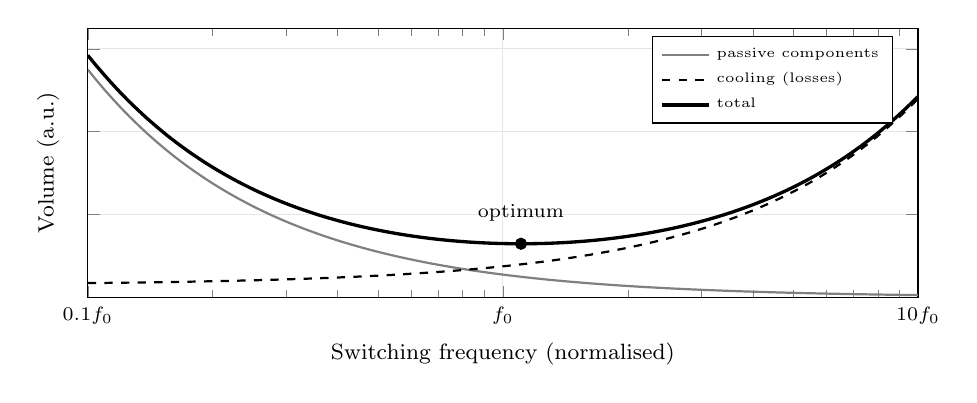
\begin{tikzpicture}
					\begin{semilogxaxis}[
							width=\linewidth, height=5.0cm,
							xmin=0.1, xmax=10, ymin=0, ymax=6.5,
							xlabel={Switching frequency (normalised)}, ylabel={Volume (a.u.)},
							xtick={0.1,1,10}, xticklabels={$0.1f_0$,$f_0$,$10f_0$}, yticklabels={},
							grid=major, grid style={gray!20},
							tick label style={font=\scriptsize}, label style={font=\footnotesize},
							legend style={font=\tiny}, legend pos=north east, legend cell align=left,
						]
						\addplot[gray, thick, domain=0.1:10, samples=100] {0.55/x};
						\addlegendentry{passive components}
						\addplot[black, thick, dashed, domain=0.1:10, samples=100] {0.3+0.45*x};
						\addlegendentry{cooling (losses)}
						\addplot[black, very thick, domain=0.1:10, samples=200] {0.55/x+0.3+0.45*x};
						\addlegendentry{total}
						\addplot[only marks, mark=*, mark size=2pt, forget plot] coordinates {(1.1055,1.295)};
						\node[font=\scriptsize, anchor=south] at (axis cs:1.1055,1.6) {optimum};
					\end{semilogxaxis}
				\end{tikzpicture}
				\caption{Qualitative trade-off: passive volume falls with $1/f_\mathrm{sw}$, the heat sink grows with the switching losses}
			\end{figure}
		\end{column}
		\begin{column}{0.5\textwidth}
			\small
			Volume-optimal $f_\mathrm{sw}$ of classical designs:
			\begin{itemize}
				\item 5\,kW isolated dc--dc converter: 28\,kW/dm$^3$ at 300\,kHz
				\item 10\,kW three-phase PFC rectifier: 44\,kW/dm$^3$ at 820\,kHz
			\end{itemize}
			Efficiency $\eta$ and power density $\rho$ conflict. Each design on the $\eta$--$\rho$ Pareto front is optimal for some weighting, and $f_\mathrm{sw}$ is one of the design variables.\\[0.3em]
			\textbf{Little Box Challenge} (Google/IEEE, 2014--16): 2\,kVA PV inverter, $\eta_\mathrm{CEC}>95\,\%$, case below 60\,$^\circ$C, target above 50\,W/in$^3$ ($\approx$ 3\,kW/dm$^3$). An ETH design study later reached 14.7\,kW/dm$^3$ at 98.1\,\% efficiency.
		\end{column}
	\end{columns}
	\blfootnote{Sources: Kolar et al., IEEJ Trans. Ind. Appl., 2008; Neumayr et al., CPSS Trans. Power Electron. Appl., vol. 5, no. 2, 2020.}
\end{frame}

%%%%%%%%%%%%%%%%%%%%%%%%%%%%%%%%%%%%%%%%%%%%%%%%%%%%%%%%%%%%%
%% What gets smaller with frequency %%
%%%%%%%%%%%%%%%%%%%%%%%%%%%%%%%%%%%%%%%%%%%%%%%%%%%%%%%%%%%%%
\subsection{What gets smaller with frequency}

\begin{frame}
	\frametitle{Energy per switching cycle}
	\begin{columns}[T]
		\begin{column}{0.5\textwidth}
			\begin{figure}
				\centering
				\begin{circuitikz}[scale=0.74, transform shape]
					\draw (0,0) to[V, l=$V_\mathrm{in}$] (0,2.6)
					to[short] (0.4,2.6) to[nos, l=$S_1$] (2.2,2.6)
					to[short, -*] (2.6,2.6) coordinate (sw)
					to[L, l=$L$, i>^=$i_L$] (4.8,2.6)
					to[short, -*] (5.2,2.6) coordinate (out)
					to[short] (6.6,2.6) to[R, l=$R$] (6.6,0) -- (0,0);
					\draw (sw) to[nos, l_=$S_2$] (2.6,0) node[circ] {};
					\draw (out) to[C, l_=$C$] (5.2,0) node[circ] {};
					\draw (7.4,2.6) to[open, v^=$V_\mathrm{o}$] (7.4,0);
				\end{circuitikz}
				\caption{Buck converter in continuous conduction mode (CCM)}
			\end{figure}
			Energy processed per cycle: $W=P/f_\mathrm{sw}$, e.g.\ 100\,W at 100\,kHz $\rightarrow$ 1\,mJ, at 10\,MHz $\rightarrow$ 10\,$\mu$J.
		\end{column}
		\begin{column}{0.47\textwidth}
			For a given current ripple $\Delta I_L$ and voltage ripple $\Delta V_\mathrm{o}$ (CCM):
			\begin{align*}
				L & =\frac{V_\mathrm{o}(1-D)}{f_\mathrm{sw}\,\Delta I_L}\propto\frac{1}{f_\mathrm{sw}} \\
				C & =\frac{\Delta I_L}{8 f_\mathrm{sw}\,\Delta V_\mathrm{o}}\propto\frac{1}{f_\mathrm{sw}}
			\end{align*}
			The peak inductor energy $\frac12 L\hat{i}_L^2$ falls with $1/f_\mathrm{sw}$ as well, since $\hat{i}_L=I_\mathrm{o}+\Delta I_L/2$ is fixed.
		\end{column}
	\end{columns}
	\begin{block}{Key message}
		Higher $f_\mathrm{sw}$ reduces the required inductance and capacitance. It does not automatically reduce the size of the component.
	\end{block}
\end{frame}

%%%%%%%%%%%%%%%%%%%%%%%%%%%%%%%%%%%%%%%%%%%%%%%%%%%%%%%%%%%%%
%% Your turn: buck inductor at 100 kHz and 2 MHz %%
%%%%%%%%%%%%%%%%%%%%%%%%%%%%%%%%%%%%%%%%%%%%%%%%%%%%%%%%%%%%%
\begin{frame}<handout:1-2>
	\frametitle{Buck inductor sizing}
	\begin{block}{Task (4 minutes)}
		Buck converter 48\,V $\rightarrow$ 12\,V, 10\,A, inductor ripple $\Delta I_L=3$\,A (30\,\%), output ripple $\Delta V_\mathrm{o}=120$\,mV (1\,\%).
		\begin{enumerate}
			\item Calculate $L$ and $C$ at 100\,kHz and at 2\,MHz.
			\item Is the 2\,MHz inductor 20 times smaller?
		\end{enumerate}
	\end{block}
	\onslide<2-|handout:2>{
		\begin{enumerate}
			\item $D=0.25$: $L=30\,\mu$H $\rightarrow$ 1.5\,$\mu$H and $C=31.3\,\mu$F $\rightarrow$ 1.56\,$\mu$F.
			\item No, far from it:
			      \begin{itemize}
				      \item the winding still carries 10\,A DC, so the conductor cross-section does not shrink with $f_\mathrm{sw}$;
				      \item same core with $\sqrt{20}$ fewer turns: $\Delta B$ falls by $\sqrt{20}$, but the core loss density $\propto f^{\alpha}\Delta B^{\beta}$ rises by $20^{1.5}\cdot 20^{-1.3}\approx 1.8$ (ferrite, $\alpha\approx1.5$, $\beta\approx2.6$);
				      \item the skin depth falls from 209\,$\mu$m to 47\,$\mu$m, so the AC resistance of the winding rises.
			      \end{itemize}
			      The magnetics frames later in this lecture explain why.
		\end{enumerate}
	}
\end{frame}

%%%%%%%%%%%%%%%%%%%%%%%%%%%%%%%%%%%%%%%%%%%%%%%%%%%%%%%%%%%%%
%% EMI filter and control bandwidth %%
%%%%%%%%%%%%%%%%%%%%%%%%%%%%%%%%%%%%%%%%%%%%%%%%%%%%%%%%%%%%%
\begin{frame}
	\frametitle{EMI filter and control bandwidth}
	\begin{columns}[T]
		\begin{column}{0.5\textwidth}
			\begin{figure}
				\centering
				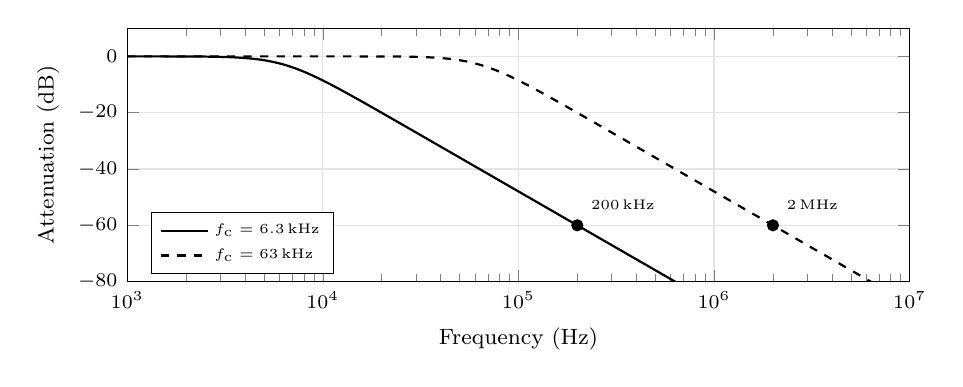
\begin{tikzpicture}
					\begin{semilogxaxis}[
							width=0.95\linewidth, height=4.8cm,
							xmin=1e3, xmax=1e7, ymin=-80, ymax=10,
							xlabel={Frequency (Hz)}, ylabel={Attenuation (dB)},
							grid=major, grid style={gray!20},
							tick label style={font=\scriptsize}, label style={font=\footnotesize},
							legend style={font=\tiny}, legend pos=south west, legend cell align=left,
						]
						\addplot[black, thick, domain=3:7, samples=200] ({10^x}, {-10*log10((1-(10^x/6324.6)^2)^2+(1.4*10^x/6324.6)^2)});
						\addlegendentry{$f_\mathrm{c}=6.3$\,kHz}
						\addplot[black, thick, dashed, domain=3:7, samples=200] ({10^x}, {-10*log10((1-(10^x/63246)^2)^2+(1.4*10^x/63246)^2)});
						\addlegendentry{$f_\mathrm{c}=63$\,kHz}
						\addplot[only marks, mark=*, mark size=2pt, forget plot] coordinates {(2e5,-60) (2e6,-60)};
						\node[font=\tiny, anchor=south west] at (axis cs:2.1e5,-58) {200\,kHz};
						\node[font=\tiny, anchor=south west] at (axis cs:2.1e6,-58) {2\,MHz};
					\end{semilogxaxis}
				\end{tikzpicture}
				\caption{Second-order LC filter ($\zeta=0.7$) providing 60\,dB at $f_\mathrm{sw}$}
			\end{figure}
		\end{column}
		\begin{column}{0.47\textwidth}
			\small
			\textbf{EMI filter:} the filter must attenuate the lowest switching harmonic in the regulated band (150\,kHz--30\,MHz for conducted emissions). With $-40$\,dB/dec, a filter giving $A$ (dB) at $f_\mathrm{sw}$ has its corner at $f_\mathrm{c}=f_\mathrm{sw}/10^{A/40}$. Ten times $f_\mathrm{sw}$ allows ten times $f_\mathrm{c}$, i.e.\ 100 times smaller $LC$. Perreault: ``It's not a bug, it's a feature!''\\[0.4em]
			\textbf{Control:} the crossover frequency $f_\mathrm{co}$ is typically $f_\mathrm{sw}/10$ to $f_\mathrm{sw}/5$. Near crossover $Z_\mathrm{out}\approx 1/(2\pi f_\mathrm{co}C)$, so a 100\,A load step with 30\,mV deviation needs 10.6\,mF at $f_\mathrm{co}=50$\,kHz but only 1.06\,mF at 500\,kHz.
		\end{column}
	\end{columns}
	\blfootnote{Source: Perreault, APEC 2024 plenary.}
\end{frame}

%%%%%%%%%%%%%%%%%%%%%%%%%%%%%%%%%%%%%%%%%%%%%%%%%%%%%%%%%%%%%
%% What does not shrink %%
%%%%%%%%%%%%%%%%%%%%%%%%%%%%%%%%%%%%%%%%%%%%%%%%%%%%%%%%%%%%%
\subsection{What does not shrink so easily}

\begin{frame}
	\frametitle{Scaling laws of magnetics}
	\begin{columns}[T]
		\begin{column}{0.5\textwidth}
			\begin{figure}
				\centering
				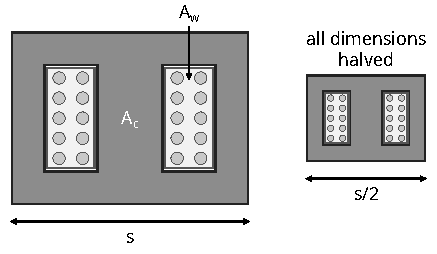
\includegraphics[width=\linewidth]{fig/lec01/core_scaling.pdf}
				\caption{An EE core scaled by $\alpha=1/2$ in every dimension ($A_\mathrm{c}$: core cross-section, $A_\mathrm{w}$: winding window)}
			\end{figure}
		\end{column}
		\begin{column}{0.47\textwidth}
			Power handling of a core with flux density $\hat{B}$ and current density $J$ (both set by losses):
			\begin{equation*}
				VA\propto f\,\hat{B}\,J\,A_\mathrm{c}A_\mathrm{w}
			\end{equation*}
			Scaling all dimensions by $\alpha$:
			\begin{itemize}
				\item $A_\mathrm{c}A_\mathrm{w}\propto\alpha^4$, volume $\propto\alpha^3$
				\item power density $\propto\alpha$: smaller is worse
				\item at constant loss density, loss/$VA\propto 1/\alpha$
			\end{itemize}
			Example: 100 transformers of 1\,W instead of one of 100\,W need $\alpha=100^{-1/4}\approx0.32$, i.e.\ $100\,\alpha^3\approx3.2$ times the volume and, at the same loss density, 3.2 times the loss.
		\end{column}
	\end{columns}
	\blfootnote{Source: C.\,R. Sullivan et al., ``On size and magnetics: Why small efficient power inductors are rare,'' 3D-PEIM 2016.}
\end{frame}

\begin{frame}
	\frametitle{Performance factor of magnetic materials}
	\begin{columns}[T]
		\begin{column}{0.5\textwidth}
			\begin{figure}
				\centering
				\begin{tikzpicture}
					\begin{semilogxaxis}[
							width=\linewidth, height=4.3cm,
							xmin=1.5, xmax=25, ymin=0, ymax=160,
							xtick={2,5,10,20}, xticklabels={2,5,10,20},
							xlabel={Frequency (MHz)}, ylabel={$\hat{B}f$ (mT$\cdot$MHz)},
							grid=major, grid style={gray!20},
							tick label style={font=\scriptsize}, label style={font=\footnotesize},
							legend style={font=\tiny, at={(0.5,-0.4)}, anchor=north, legend columns=2, /tikz/every even column/.append style={column sep=0.25cm}}, legend cell align=left,
							unbounded coords=jump,
						]
						\addplot[black, thick, mark=*, mark size=1.5pt] table[x=f_MHz, y=FR67] {fig/lec01/data/pf_hanson2016_Pv500.dat};
						\addlegendentry{67, $\mu_\mathrm{r}=40$}
						\addplot[black, thick, dashed, mark=square*, mark size=1.5pt] table[x=f_MHz, y=M3] {fig/lec01/data/pf_hanson2016_Pv500.dat};
						\addlegendentry{M3, $\mu_\mathrm{r}=20$}
						\addplot[gray, thick, mark=triangle*, mark size=1.8pt] table[x=f_MHz, y=F4F1] {fig/lec01/data/pf_hanson2016_Pv500.dat};
						\addlegendentry{4F1, $\mu_\mathrm{r}=80$}
						\addplot[gray, thick, dashed, mark=o, mark size=1.5pt] table[x=f_MHz, y=FR61] {fig/lec01/data/pf_hanson2016_Pv500.dat};
						\addlegendentry{61, $\mu_\mathrm{r}=125$}
					\end{semilogxaxis}
				\end{tikzpicture}
				\caption{Performance factor at $P_\mathrm{v}=500$\,mW/cm$^3$ from the Steinmetz fits of Hanson et al.\ (2016): Fair-Rite 67, 61; Nat.\ Magnetics M3; Ferroxcube 4F1}
			\end{figure}
		\end{column}
		\begin{column}{0.47\textwidth}
			\small
			At high frequency $\hat{B}$ is limited by core loss, not by saturation. With the Steinmetz fit $P_\mathrm{v}=k\hat{B}^{\beta}$ at each frequency:
			\begin{equation*}
				\hat{B}=\left(\frac{P_\mathrm{v}}{k}\right)^{1/\beta},\qquad PF=\hat{B}\,f
			\end{equation*}
			\begin{itemize}
				\item At fixed size and loss density, $VA\propto PF$.
				\item $PF$ rises with $f$ only up to a material-specific limit, here 10--15\,MHz.
				\item With available materials, $PF$ keeps improving up to about 30\,MHz (Perreault, 2024).
				\item With skin effect in a single-layer winding, $\hat{B}f^{3/4}$ is the fairer metric (L6).
			\end{itemize}
		\end{column}
	\end{columns}
\end{frame}

%%%%%%%%%%%%%%%%%%%%%%%%%%%%%%%%%%%%%%%%%%%%%%%%%%%%%%%%%%%%%
%% Device losses %%
%%%%%%%%%%%%%%%%%%%%%%%%%%%%%%%%%%%%%%%%%%%%%%%%%%%%%%%%%%%%%
\begin{frame}
	\frametitle{Power semiconductor devices}
	\begin{table}
		\centering
		\small
		\begin{tabular}{|l|l|>{\raggedright\arraybackslash}p{6.2cm}|}
			\hline
			\textbf{Mechanism}                    & \textbf{Energy per period}                  & \textbf{Remark}                                                     \\
			\hline
			$V$--$I$ overlap (hard switching)     & $\frac12 VI(t_\mathrm{r}+t_\mathrm{f})$      & set by drive strength, $\mathrm{d}i/\mathrm{d}t$, $\mathrm{d}v/\mathrm{d}t$ \\
			$C_\mathrm{oss}$ charging (hard turn-on) & $Q_\mathrm{oss}V_\mathrm{DC}$            & present even with an infinitely fast switch                         \\
			Reverse recovery                      & $\approx Q_\mathrm{rr}V_\mathrm{DC}$          & Si body diodes; none for GaN, small for SiC                         \\
			Gate drive (per switch)               & $Q_\mathrm{G}V_\mathrm{dr}$                  & dissipated in the driver and gate resistors                         \\
			Dead-time conduction                  & $2V_\mathrm{SD}I\,t_\mathrm{d}$              & GaN conducts in reverse at a few volts                              \\
			$C_\mathrm{oss}$ hysteresis           & $E_\mathrm{hyst}$                            & remains with soft switching, may exceed conduction loss at MHz      \\
			\hline
		\end{tabular}
		\caption{Switching-related loss mechanisms, all multiplied by $f_\mathrm{sw}$}
	\end{table}
	Conduction loss $I^2R_\mathrm{DS(on)}$ does not depend on $f_\mathrm{sw}$. Every term in the table does. L2 turns this table into a complete loss model.
	\blfootnote{$C_\mathrm{oss}$ hysteresis: Fedison et al., APEC 2014; Zulauf et al., TPEL 2018; Perreault, APEC 2024.}
\end{frame}

\begin{frame}
	\frametitle{Switching versus conduction loss}
	\begin{columns}[T]
		\begin{column}{0.55\textwidth}
			\begin{figure}
				\centering
				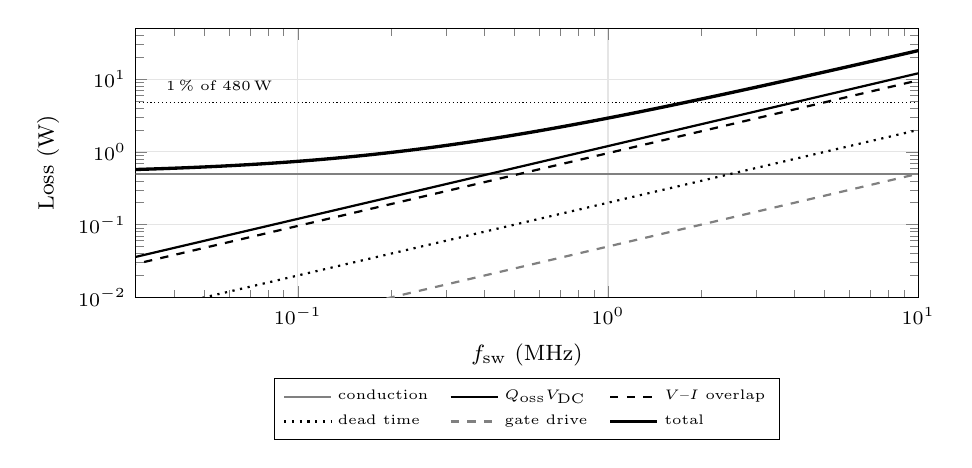
\begin{tikzpicture}
					\begin{loglogaxis}[
							width=0.95\linewidth, height=5.0cm,
							xmin=0.03, xmax=10, ymin=0.01, ymax=50,
							xlabel={$f_\mathrm{sw}$ (MHz)}, ylabel={Loss (W)},
							grid=major, grid style={gray!20},
							tick label style={font=\scriptsize}, label style={font=\footnotesize},
							legend style={font=\tiny, at={(0.5,-0.3)}, anchor=north, legend columns=3, /tikz/every even column/.append style={column sep=0.2cm}}, legend cell align=left,
						]
						\addplot[gray, thick, domain=-1.6:1, samples=2] ({10^x}, {0.5});
						\addlegendentry{conduction}
						\addplot[black, thick, domain=-1.6:1, samples=2] ({10^x}, {1.2*10^x});
						\addlegendentry{$Q_\mathrm{oss}V_\mathrm{DC}$}
						\addplot[black, thick, dashed, domain=-1.6:1, samples=2] ({10^x}, {0.96*10^x});
						\addlegendentry{$V$--$I$ overlap}
						\addplot[black, thick, dotted, domain=-1.6:1, samples=2] ({10^x}, {0.2*10^x});
						\addlegendentry{dead time}
						\addplot[gray, thick, dashed, domain=-1.6:1, samples=2] ({10^x}, {0.05*10^x});
						\addlegendentry{gate drive}
						\addplot[black, very thick, domain=-1.6:1, samples=60] ({10^x}, {0.5+2.41*10^x});
						\addlegendentry{total}
						\addplot[black, densely dotted, domain=-1.6:1, samples=2, forget plot] ({10^x}, {4.8});
						\node[font=\tiny, anchor=south west] at (axis cs:0.035,5.0) {1\,\% of 480\,W};
					\end{loglogaxis}
				\end{tikzpicture}
				\caption{Hard-switched 48\,V, 10\,A GaN half-bridge (illustrative values)}
			\end{figure}
		\end{column}
		\begin{column}{0.42\textwidth}
			\small
			Assumed values (not a specific device):
			\begin{itemize}
				\item $R_\mathrm{DS(on)}=5$\,m$\Omega$
				\item $Q_\mathrm{oss}=25$\,nC at 48\,V
				\item $t_\mathrm{r}+t_\mathrm{f}=4$\,ns
				\item $t_\mathrm{d}=5$\,ns, $V_\mathrm{SD}=2$\,V
				\item $Q_\mathrm{G}=5$\,nC per switch, $V_\mathrm{dr}=5$\,V
			\end{itemize}
			Switching loss equals conduction loss at about 200\,kHz. The total loss reaches 1\,\% of the output power (4.8\,W) at about 1.8\,MHz. Above that, every further increase of $f_\mathrm{sw}$ costs efficiency directly.
		\end{column}
	\end{columns}
\end{frame}

%%%%%%%%%%%%%%%%%%%%%%%%%%%%%%%%%%%%%%%%%%%%%%%%%%%%%%%%%%%%%
%% Parasitics %%
%%%%%%%%%%%%%%%%%%%%%%%%%%%%%%%%%%%%%%%%%%%%%%%%%%%%%%%%%%%%%
\begin{frame}
	\frametitle{Parasitics at high frequency}
	\begin{columns}[T]
		\begin{column}{0.42\textwidth}
			\begin{figure}
				\centering
				\begin{circuitikz}[scale=0.7, transform shape]
					% transistors of the half-bridge
					\draw (3,3.75) node[nigfete](T1){} (3,1.25) node[nigfete](T2){};
					\draw (T1) node[anchor=west]{$S_1$};
					\draw (T2) node[anchor=west]{$S_2$};
					% commutation loop: DC-link capacitor and loop inductance
					\draw (0,0) to[C, l=$C_\mathrm{DC}$] (0,5) to[L, l=$L_{\sigma1}$] (3,5) -- (T1.D);
					\draw (T1.S) -- (T2.D);
					\draw (T2.S) -- (3,0) to[L, l=$L_{\sigma2}$] (0,0);
					% switch node: load current and capacitance to the heat sink
					\draw (3,2.5) to[short, *-*] (4.2,2.5) to[short, i=$I_\mathrm{L}$, -o] (5.6,2.5);
					\draw (4.2,2.5) to[C, l=$C_\mathrm{p}$] (4.2,0.9) node[ground]{};
				\end{circuitikz}
				\caption{Half-bridge with loop inductance $L_\mathrm{loop}=L_{\sigma1}+L_{\sigma2}$ and switch-node capacitance $C_\mathrm{p}$ to the heat sink}
			\end{figure}
		\end{column}
		\begin{column}{0.55\textwidth}
			\small
			Layout and package set the parasitics, not $f_\mathrm{sw}$. Fast edges make them visible:
			\begin{itemize}
				\item overshoot $\Delta v=L_\mathrm{loop}\,\mathrm{d}i/\mathrm{d}t$: 2\,nH, 10\,A in 2\,ns $\rightarrow$ 10\,V
				\item ringing $f_\mathrm{r}=1/\big(2\pi\sqrt{L_\mathrm{loop}C_\mathrm{oss}}\big)$: 2\,nH, 200\,pF $\rightarrow$ 250\,MHz
				\item common-mode current $i=C_\mathrm{p}\,\mathrm{d}v/\mathrm{d}t$: 10\,pF, 100\,V/ns $\rightarrow$ 1\,A
				\item spectrum envelope falls with $-40$\,dB/dec above $1/(\pi t_\mathrm{r})$: 160\,MHz for $t_\mathrm{r}=2$\,ns
			\end{itemize}
			\begin{block}{Key message}
				A ringing of 10\,ns is 0.1\,\% of the period at 100\,kHz but 10\,\% at 10\,MHz. L3 shows how to make the loop small.
			\end{block}
		\end{column}
	\end{columns}
\end{frame}

%%%%%%%%%%%%%%%%%%%%%%%%%%%%%%%%%%%%%%%%%%%%%%%%%%%%%%%%%%%%%
%% Skin effect %%
%%%%%%%%%%%%%%%%%%%%%%%%%%%%%%%%%%%%%%%%%%%%%%%%%%%%%%%%%%%%%
\begin{frame}
	\frametitle{Skin effect in windings}
	\begin{columns}[T]
		\begin{column}{0.5\textwidth}
			\begin{figure}
				\centering
				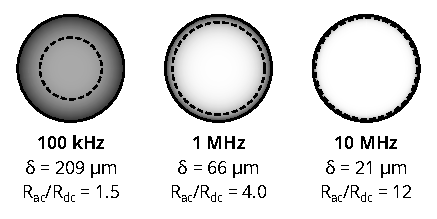
\includegraphics[width=\linewidth]{fig/lec01/skin_effect_wire.pdf}
				\caption{Current density in a round copper wire, 1\,mm diameter, 20\,$^\circ$C (exact solution; darker means higher $|J|$, dashed: one skin depth below the surface)}
			\end{figure}
		\end{column}
		\begin{column}{0.47\textwidth}
			Skin depth of copper:
			\begin{equation*}
				\delta=\sqrt{\frac{\rho}{\pi f \mu_0}}\approx\frac{66\,\mu\mathrm{m}}{\sqrt{f/\mathrm{MHz}}}\quad(20\,^\circ\mathrm{C})
			\end{equation*}
			\small
			\begin{itemize}
				\item 1\,oz PCB copper (35\,$\mu$m) equals $\delta$ at 3.6\,MHz.
				\item At 100\,$^\circ$C: $\rho$ +31\,\%, $\delta$ +15\,\%.
				\item In multilayer windings the proximity effect adds far more loss (Dowell, L7).
				\item Litz wire loses its advantage above a few MHz: the finest strands (50\,AWG, 25\,$\mu$m) equal $\delta$ at 7\,MHz.
			\end{itemize}
		\end{column}
	\end{columns}
	\blfootnote{Sources: Perreault, APEC 2024 plenary; Dowell, Proc. IEE, 1966.}
\end{frame}

%%%%%%%%%%%%%%%%%%%%%%%%%%%%%%%%%%%%%%%%%%%%%%%%%%%%%%%%%%%%%
%% Your turn: skin depth %%
%%%%%%%%%%%%%%%%%%%%%%%%%%%%%%%%%%%%%%%%%%%%%%%%%%%%%%%%%%%%%
% Two pages: task (page 1) and task with solution (page 2).
\begin{frame}<handout:1-2>
	\frametitle{Skin depth at 6.78\,MHz}
	\begin{block}{Task (3 minutes)}
		A single-layer copper foil winding carries a 6.78\,MHz current. The magnetic field is on one side of the foil only.
		\begin{enumerate}
			\item Skin depth of copper at 20\,$^\circ$C?
			\item Which copper thickness do you choose: 1\,oz (35\,$\mu$m) or 2\,oz (70\,$\mu$m)?
		\end{enumerate}
	\end{block}
	\onslide<2-|handout:2>{
		\begin{enumerate}
			\item $\delta=66\,\mu\mathrm{m}/\sqrt{6.78}\approx 25\,\mu$m.
			\item 1\,oz. For a single layer with the field on one side, the AC resistance is lowest at a thickness of $\frac{\pi}{2}\delta\approx 40\,\mu$m. 1\,oz is within 2\,\% of this optimum. 2\,oz gives about 7.5\,\% more AC resistance than 1\,oz: the extra copper carries almost no current. The derivation follows in L7 (Dowell).
		\end{enumerate}
	}
\end{frame}

%%%%%%%%%%%%%%%%%%%%%%%%%%%%%%%%%%%%%%%%%%%%%%%%%%%%%%%%%%%%%
%% Timing %%
%%%%%%%%%%%%%%%%%%%%%%%%%%%%%%%%%%%%%%%%%%%%%%%%%%%%%%%%%%%%%
\begin{frame}
	\frametitle{Timing at high frequency}
	\begin{columns}[T]
		\begin{column}{0.47\textwidth}
			\begin{figure}
				\centering
				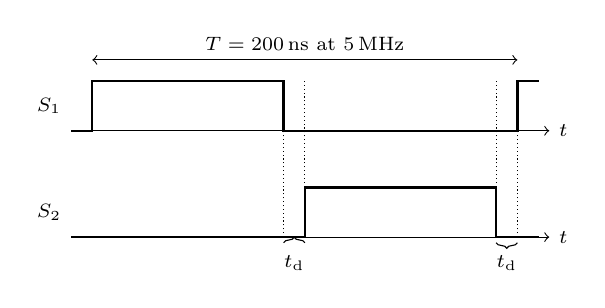
\begin{tikzpicture}[x=0.027cm, y=0.9cm]
					% time axes
					\draw[->] (0,0) -- (225,0) node[right, font=\scriptsize] {$t$};
					\draw[->] (0,1.5) -- (225,1.5) node[right, font=\scriptsize] {$t$};
					% gate signal S1 (high side): on from 10 ns to 100 ns and from 210 ns
					\draw[thick] (0,1.5) -- (10,1.5) -- (10,2.2) -- (100,2.2) -- (100,1.5) -- (210,1.5) -- (210,2.2) -- (220,2.2);
					% gate signal S2 (low side): on from 110 ns to 200 ns
					\draw[thick] (0,0) -- (110,0) -- (110,0.7) -- (200,0.7) -- (200,0) -- (220,0);
					\node[anchor=east, font=\scriptsize] at (0,1.85) {$S_1$};
					\node[anchor=east, font=\scriptsize] at (0,0.35) {$S_2$};
					% dead times
					\draw[densely dotted] (100,0) -- (100,2.2) (110,0) -- (110,2.2);
					\draw[densely dotted] (200,0) -- (200,2.2) (210,0) -- (210,2.2);
					\draw[decorate, decoration={brace, amplitude=2pt}] (100,-0.08) -- (110,-0.08) node[pos=0.5, below=1pt, font=\scriptsize] {$t_\mathrm{d}$};
					\draw[decorate, decoration={brace, mirror, amplitude=2pt}] (200,-0.08) -- (210,-0.08) node[pos=0.5, below=1pt, font=\scriptsize] {$t_\mathrm{d}$};
					% period
					\draw[<->] (10,2.5) -- node[above, font=\scriptsize] {$T=200$\,ns at 5\,MHz} (210,2.5);
				\end{tikzpicture}
				\caption{Gate signals of a half-bridge at 5\,MHz with $t_\mathrm{d}=10$\,ns (to scale)}
			\end{figure}
		\end{column}
		\begin{column}{0.5\textwidth}
			\small
			\begin{itemize}
				\item Two dead times of 10\,ns already take 10\,\% of the period at 5\,MHz.
				\item Drivers and digital isolators add delays of tens of ns. Their part-to-part spread must fit into the dead time.
				\item A duty-cycle resolution of 0.1\,\% at 5\,MHz needs a time step of 0.2\,ns, i.e.\ a 5\,GHz counter or a high-resolution PWM unit.
				\item Isolated drivers must tolerate the switch-node $\mathrm{d}v/\mathrm{d}t$: their common-mode transient immunity (CMTI) must exceed e.g.\ 100\,V/ns.
			\end{itemize}
			Sensing and control are often not the limit. If they are, avoid controls that need low latency (L13).
		\end{column}
	\end{columns}
	\blfootnote{Source: Perreault, APEC 2024 plenary.}
\end{frame}

%%%%%%%%%%%%%%%%%%%%%%%%%%%%%%%%%%%%%%%%%%%%%%%%%%%%%%%%%%%%%
%% Quiz: what limits miniaturisation %%
%%%%%%%%%%%%%%%%%%%%%%%%%%%%%%%%%%%%%%%%%%%%%%%%%%%%%%%%%%%%%
% Two pages: question (page 1) and answer (page 2).
\begin{frame}<handout:1-2>
	\frametitle{What limits miniaturisation?}
	A 1\,kW converter is redesigned from 100\,kHz to 10\,MHz. Which two items limit the size reduction most? Vote, then discuss with your neighbour (2 minutes).
	\begin{enumerate}[(a)]
		\item the control loop and the sensing
		\item the magnetic components
		\item the device losses ($C_\mathrm{oss}$ loss, dynamic $R_\mathrm{DS(on)}$)
		\item the EMI filter
	\end{enumerate}
	\onslide<2-|handout:2>{
		\begin{block}{Answer: (b) and (c)}
			Core loss limits $\hat{B}$ and the skin effect limits the useful copper, so magnetics shrink much less than $1/f_\mathrm{sw}$. $C_\mathrm{oss}$ losses remain with soft switching and can exceed the conduction loss. The EMI filter becomes smaller as $f_\mathrm{sw}$ rises, and sensing and control are often not the limiting factor.
		\end{block}
	}
	\blfootnote{Source: Perreault, APEC 2024 plenary.}
\end{frame}

%%%%%%%%%%%%%%%%%%%%%%%%%%%%%%%%%%%%%%%%%%%%%%%%%%%%%%%%%%%%%
%% Summary table %%
%%%%%%%%%%%%%%%%%%%%%%%%%%%%%%%%%%%%%%%%%%%%%%%%%%%%%%%%%%%%%
\begin{frame}
	\frametitle{Summary of scaling laws}
	\begin{table}
		\centering
		\small
		\begin{tabular}{|l|l|>{\raggedright\arraybackslash}p{5.9cm}|}
			\hline
			\textbf{Quantity}                     & \textbf{Scaling}                   & \textbf{Remark}                                                      \\
			\hline
			Required $L$ and $C$                  & $\propto 1/f_\mathrm{sw}$          & for a given ripple                                                   \\
			EMI filter $LC$                       & $\propto 1/f_\mathrm{sw}^2$        & for a given attenuation at $f_\mathrm{sw}$                           \\
			Control bandwidth                     & $\propto f_\mathrm{sw}$            & crossover at about $f_\mathrm{sw}/10$                                \\
			Hard-switching loss                   & $\propto f_\mathrm{sw}$            & $Q_\mathrm{oss}V_\mathrm{DC}$, overlap, gate charge, dead time       \\
			Core loss density at fixed $\hat{B}$  & $\propto f_\mathrm{sw}^{\alpha}$   & $\alpha\approx 1.4$--$2$ for ferrites, so $\hat{B}$ must fall         \\
			Power density of magnetics            & rises, then falls                  & optimum at 10--30\,MHz, set by the material                          \\
			Skin depth                            & $\propto 1/\sqrt{f_\mathrm{sw}}$   & $R_\mathrm{ac}$ rises, litz wire loses its advantage                 \\
			Parasitics, delays, dead time         & fixed in ns                        & their share of the period grows with $f_\mathrm{sw}$                 \\
			Conduction loss                       & independent                        & $I^2R_\mathrm{DS(on)}$                                               \\
			\hline
		\end{tabular}
		\caption{First-order scaling laws of this lecture ($\alpha$ after Perreault et al., 2009)}
	\end{table}
\end{frame}

%%%%%%%%%%%%%%%%%%%%%%%%%%%%%%%%%%%%%%%%%%%%%%%%%%%%%%%%%%%%%
%% Consequences and roadmap %%
%%%%%%%%%%%%%%%%%%%%%%%%%%%%%%%%%%%%%%%%%%%%%%%%%%%%%%%%%%%%%
\subsection{Consequences and course roadmap}

\begin{frame}
	\frametitle{Need for soft switching}
	\begin{columns}[T]
		\begin{column}{0.52\textwidth}
			Capacitive switching loss relative to the output power:
			\begin{equation*}
				\frac{P_\mathrm{Qoss}}{P_\mathrm{o}}=\frac{Q_\mathrm{oss}V_\mathrm{DC}f_\mathrm{sw}}{P_\mathrm{o}}
			\end{equation*}
			For the 650\,V GaN device at 400\,V and 1\,kW, this reaches 1\,\% at 625\,kHz.\\[0.2em]
			Three ways to raise $f_\mathrm{sw}$ anyway:
			\begin{enumerate}
				\item zero-voltage switching: an inductive current commutates the switch-node voltage before the switch turns on (L8--L10)
				\item lower voltage per switch: multilevel, stacked and switched-capacitor converters (L12)
				\item better devices: less $Q_\mathrm{oss}$ and $C_\mathrm{oss}$ hysteresis for the same $R_\mathrm{DS(on)}$ (L2)
			\end{enumerate}
		\end{column}
		\begin{column}{0.45\textwidth}
			\begin{block}{What soft switching does not remove}
				\begin{itemize}
					\item $C_\mathrm{oss}$ hysteresis loss
					\item gate-drive loss
					\item core and winding loss
					\item conduction loss of the circulating current
				\end{itemize}
			\end{block}
			Hence the commutation cell, gate drive, measurement and magnetics (L2--L7) come before the soft-switching and resonant topologies (L8--L10).
		\end{column}
	\end{columns}
\end{frame}

%%%%%%%%%%%%%%%%%%%%%%%%%%%%%%%%%%%%%%%%%%%%%%%%%%%%%%%%%%%%%
%% Course roadmap %%
%%%%%%%%%%%%%%%%%%%%%%%%%%%%%%%%%%%%%%%%%%%%%%%%%%%%%%%%%%%%%
\begin{frame}
	\frametitle{Course roadmap}
	\begin{columns}[T]
		\begin{column}{0.49\textwidth}
			\footnotesize
			\begin{tabular}{|l|l|>{\raggedright\arraybackslash}p{4.7cm}|}
				\hline
				L1 & 13.10. & Why high switching frequency?                                  \\
				L2 & 20.10. & HF switching cell: losses and devices     \\
				L3 & 27.10. & Parasitics and PCB layout              \\
				L4 & 03.11. & Gate drivers for fast-switching devices                        \\
				L5 & 10.11. & Measurement and characterisation                         \\
				L6 & 17.11. & HF magnetics I: materials, core loss       \\
				L7 & 24.11. & HF magnetics II: windings, planar      \\
				L8 & 01.12. & Soft switching without resonance                               \\
				\hline
			\end{tabular}
		\end{column}
		\begin{column}{0.49\textwidth}
			\footnotesize
			\begin{tabular}{|l|l|>{\raggedright\arraybackslash}p{4.7cm}|}
				\hline
				L9  & 08.12. & Resonant converters I: SRC, PRC, LLC, CLLC                    \\
				L10 & 15.12. & Resonant converters II: VHF, matching \\
				L11 & 22.12. & Case studies and teardown                                     \\
				L12 & 12.01. & Switched-capacitor and hybrid converters                      \\
				L13 & 19.01. & Modelling and control at HF                                   \\
				L14 & 26.01. & EMI, thermal design and integration                           \\
				L15 & 02.02. & Synthesis and exam preparation               \\
				\hline
			\end{tabular}
		\end{column}
	\end{columns}
	\vspace{0.4cm}
	Tutorials on Wednesdays, 08--10, from 14.10. Each tutorial has a Jupyter notebook. T1 starts with the frequency-scaling explorer and the set-up of Python, ngspice and KiCad.
\end{frame}

%%%%%%%%%%%%%%%%%%%%%%%%%%%%%%%%%%%%%%%%%%%%%%%%%%%%%%%%%%%%%
%% Key messages %%
%%%%%%%%%%%%%%%%%%%%%%%%%%%%%%%%%%%%%%%%%%%%%%%%%%%%%%%%%%%%%
\begin{frame}
	\frametitle{Key messages}
	\begin{enumerate}
		\item The energy per cycle falls with $1/f_\mathrm{sw}$, and so do the required $L$ and $C$. EMI filters and control bandwidth benefit even more.
		\item Components do not shrink in proportion: core loss limits $\hat{B}$, skin and proximity effect limit the useful copper, and small magnetics are inherently less efficient.
		\item Every hard switching event costs $Q_\mathrm{oss}V_\mathrm{DC}$ plus overlap, gate and dead-time energy. Somewhere between a few hundred kHz (high voltage) and a few MHz (low voltage), this energy must be recovered by soft switching.
		\item Parasitics and delays are fixed in nanoseconds and take a growing share of the period.
		\item $f_\mathrm{sw}$ is a design variable with an optimum, not a goal in itself.
	\end{enumerate}
\end{frame}

%%%%%%%%%%%%%%%%%%%%%%%%%%%%%%%%%%%%%%%%%%%%%%%%%%%%%%%%%%%%%
%% Exit ticket %%
%%%%%%%%%%%%%%%%%%%%%%%%%%%%%%%%%%%%%%%%%%%%%%%%%%%%%%%%%%%%%
% Two pages: questions (page 1) and answers (page 2).
\begin{frame}<handout:1-2>
	\frametitle{Exit ticket}
	\begin{varblock}[\textwidth]{Three questions, one minute each}
		\begin{enumerate}
			\item You raise $f_\mathrm{sw}$ from 200\,kHz to 2\,MHz. By which factor can the $LC$ product of a second-order EMI filter shrink for the same attenuation at $f_\mathrm{sw}$?
			\item Name two loss mechanisms that remain with zero-voltage switching.
			\item Skin depth of copper (20\,$^\circ$C) at 1\,MHz and at 100\,MHz?
		\end{enumerate}
	\end{varblock}
	\onslide<2-|handout:2>{
		\begin{enumerate}
			\item By 100: the corner frequency can rise by 10, and $LC\propto 1/f_\mathrm{c}^2$.
			\item Any two of: $C_\mathrm{oss}$ hysteresis, gate drive, conduction (including circulating current), core and winding loss.
			\item 66\,$\mu$m and 6.6\,$\mu$m.
		\end{enumerate}
	}
\end{frame}

%%%%%%%%%%%%%%%%%%%%%%%%%%%%%%%%%%%%%%%%%%%%%%%%%%%%%%%%%%%%%
%% Recommended reading %%
%%%%%%%%%%%%%%%%%%%%%%%%%%%%%%%%%%%%%%%%%%%%%%%%%%%%%%%%%%%%%
\begin{frame}
	\frametitle{Recommended reading}
	\small
	\begin{itemize}
		\item J.\,G. Kassakian, D.\,J. Perreault, G.\,C. Verghese, M.\,F. Schlecht, \textit{Principles of Power Electronics}, 2nd ed., Cambridge University Press, 2023.
		\item R.\,W. Erickson, D. Maksimovi\'c, \textit{Fundamentals of Power Electronics}, 3rd ed., Springer, 2020.
		\item M.\,K. Kazimierczuk, D. Czarkowski, \textit{Resonant Power Converters}, 2nd ed., Wiley, 2011.
		\item W.\,G. Hurley, W.\,H. W\"olfle, \textit{Transformers and Inductors for Power Electronics}, Wiley, 2013.
		\item A. Lidow, M. de Rooij, J. Strydom, D. Reusch, J. Glaser, \textit{GaN Transistors for Efficient Power Conversion}, 3rd ed., Wiley, 2019.
		\item F. Wang, Z. Zhang, E.\,A. Jones, \textit{Characterization of Wide Bandgap Power Semiconductor Devices}, IET, 2018.
		\item Z. Zhang, Y.-F. Liu, \textit{High Frequency MOSFET Gate Drivers}, IET, 2017.
		\item H.\,W. Ott, \textit{Electromagnetic Compatibility Engineering}, Wiley, 2009.
	\end{itemize}
	The papers used in each lecture are listed at its end.
\end{frame}

%%%%%%%%%%%%%%%%%%%%%%%%%%%%%%%%%%%%%%%%%%%%%%%%%%%%%%%%%%%%%
%% References of this lecture %%
%%%%%%%%%%%%%%%%%%%%%%%%%%%%%%%%%%%%%%%%%%%%%%%%%%%%%%%%%%%%%
\begin{frame}
	\frametitle{References}
	\scriptsize
	\begin{itemize}
		\item D.\,J. Perreault, ``Opportunities, progress and challenges in high-frequency power conversion,'' plenary talk, IEEE APEC 2024.
		\item D.\,J. Perreault et al., ``Opportunities and challenges in very high frequency power conversion,'' IEEE APEC 2009, pp.\ 1--14.
		\item J.\,W. Kolar et al., ``PWM converter power density barriers,'' IEEJ Trans.\ Ind.\ Appl., vol.\ 128, no.\ 4, pp.\ 468--480, 2008.
		\item D. Neumayr et al., ``The essence of the Little Box Challenge -- Part A: Key design challenges \& solutions,'' CPSS Trans.\ Power Electron.\ Appl., vol.\ 5, no.\ 2, pp.\ 158--179, 2020.
		\item C.\,R. Sullivan, B.\,A. Reese, A.\,L.\,F. Stein, P.\,A. Kyaw, ``On size and magnetics: Why small efficient power inductors are rare,'' 3D-PEIM 2016.
		\item A.\,J. Hanson et al., ``Measurements and performance factor comparisons of magnetic materials at high frequency,'' IEEE Trans.\ Power Electron., vol.\ 31, no.\ 11, pp.\ 7909--7925, 2016.
		\item G. Zulauf et al., ``COSS losses in 600 V GaN power semiconductors in soft-switched, high- and very-high-frequency power converters,'' IEEE Trans.\ Power Electron., vol.\ 33, no.\ 12, pp.\ 10748--10763, 2018.
		\item J.\,B. Fedison, M. Fornage, M.\,J. Harrison, D.\,R. Zimmanck, ``Coss related energy loss in power MOSFETs used in zero-voltage-switched applications,'' IEEE APEC 2014, pp.\ 150--156.
		\item P.\,L. Dowell, ``Effects of eddy currents in transformer windings,'' Proc.\ IEE, vol.\ 113, no.\ 8, pp.\ 1387--1394, 1966.
		\item Y. Zhang et al., ``Wide-bandgap semiconductors and power electronics as pathways to carbon neutrality,'' Nature Reviews Electrical Engineering, vol.\ 2, pp.\ 155--172, 2025.
	\end{itemize}
\end{frame}

\begin{frame}
	\frametitle{References (cont.)}
	\scriptsize
	Designs in the MHz table and on the power--frequency map:
	\begin{itemize}
		\item E.\,A. Burton et al., ``FIVR -- Fully integrated voltage regulators on 4th generation Intel Core SoCs,'' IEEE APEC 2014, pp.\ 432--439.
		\item Y. Elasser et al., ``Mini-LEGO: A 1.5-MHz 240-A 48-V-to-1-V CPU VRM with 8.4-mm height for vertical power delivery,'' IEEE APEC 2023, pp.\ 1959--1966.
		\item M.\,K. Ranjram, D.\,J. Perreault, ``A 380-12 V, 1-kW, 1-MHz converter using a miniaturized split-phase, fractional-turn planar transformer,'' IEEE Trans.\ Power Electron., vol.\ 37, no.\ 2, pp.\ 1666--1681, 2022.
		\item S. Lim, D.\,M. Otten, D.\,J. Perreault, ``New AC--DC power factor correction architecture suitable for high-frequency operation,'' IEEE Trans.\ Power Electron., vol.\ 31, no.\ 4, 2016.
		\item J. Santiago-Gonz\'alez et al., ``Single-phase universal-input PFC converter operating at high frequency,'' IEEE J.\ Emerg.\ Sel.\ Topics Ind.\ Electron., 2023.
		\item L. Gu et al., ``6.78-MHz wireless power transfer with self-resonant coils at 95\,\% DC--DC efficiency,'' IEEE Trans.\ Power Electron., vol.\ 36, no.\ 3, pp.\ 2456--2460, 2021.
		\item H. Zhang, ``Techniques for efficient wide-range radio-frequency power generation,'' PhD thesis, MIT, 2022.
		\item Y. Cao et al., ``Design and implementation of an 18 kW 500 kHz 98.8\,\% efficiency high-density battery charger with partial power processing,'' IEEE J.\ Emerg.\ Sel.\ Topics Power Electron., vol.\ 10, pp.\ 7963--7975, 2022.
		\item Further wireless and RF power designs on the map (Braun 2019; Al Bastami 2020; Regensburger 2022; Nikiforidis 2023) as cited in Perreault, APEC 2024.
	\end{itemize}
\end{frame}
 % Why high switching frequency? Scaling laws and the V-I-P-f map
\title[High-frequency switching cell]{The high-frequency switching cell}
\section{High-frequency switching cell}

\begin{frame}[plain]
	\titlepage
\end{frame}

%%%%%%%%%%%%%%%%%%%%%%%%%%%%%%%%%%%%%%%%%%%%%%%%%%%%%%%%%%%%%
%% Overview %%
%%%%%%%%%%%%%%%%%%%%%%%%%%%%%%%%%%%%%%%%%%%%%%%%%%%%%%%%%%%%%
\subsection{Recap from PEDC}

\begin{frame}
	\frametitle{Overview}
	Lecture 1 showed that switching losses grow with $f_\mathrm{sw}$ while conduction loss does not. This lecture looks at the first rung of the frequency ladder in detail: the losses of the switching cell itself.
	\begin{itemize}
		\item Recap: switching transitions and figures of merit (PEDC L05--L06)
		\item The output capacitance: charge, energy and hysteresis
		\item The complete loss inventory of a switching cell at MHz
		\item Hard versus soft switching and the optimum die size
		\item Device technologies and packages for high frequency
	\end{itemize}
	After this lecture you can set up a loss budget from datasheet values and choose a device for a given voltage, current and switching frequency.
\end{frame}

%%%%%%%%%%%%%%%%%%%%%%%%%%%%%%%%%%%%%%%%%%%%%%%%%%%%%%%%%%%%%
%% Switching transitions %%
%%%%%%%%%%%%%%%%%%%%%%%%%%%%%%%%%%%%%%%%%%%%%%%%%%%%%%%%%%%%%
\begin{frame}
	\frametitle{Hard turn-on transition}
	\begin{columns}[T]
		\begin{column}{0.5\textwidth}
			\begin{figure}
				\centering
				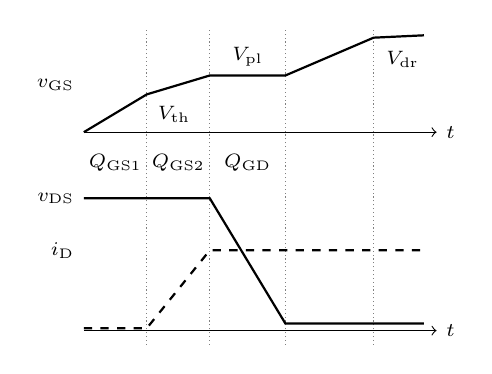
\begin{tikzpicture}[x=0.8cm, y=0.6cm, font=\scriptsize]
					% time markers
					\foreach \t in {1,2,3.2,4.6} {\draw[densely dotted, gray] (\t,-3.3) -- (\t,3.4);}
					% gate-source voltage
					\draw[->] (0,1.2) -- (5.6,1.2) node[right] {$t$};
					\draw[thick] (0,1.2) -- (1,2.0) -- (2,2.4) -- (3.2,2.4) -- (4.6,3.2) -- (5.4,3.25);
					\node[anchor=east] at (0,2.2) {$v_\mathrm{GS}$};
					\node[anchor=west] at (4.65,2.75) {$V_\mathrm{dr}$};
					\node[anchor=south] at (2.6,2.4) {$V_\mathrm{pl}$};
					\node[anchor=north west] at (1.02,1.95) {$V_\mathrm{th}$};
					% drain current and drain-source voltage
					\draw[->] (0,-3) -- (5.6,-3) node[right] {$t$};
					\draw[thick] (0,-0.2) -- (2,-0.2) -- (3.2,-2.85) -- (5.4,-2.85);
					\draw[thick, dashed] (0,-2.95) -- (1,-2.95) -- (2,-1.3) -- (5.4,-1.3);
					\node[anchor=east] at (0,-0.2) {$v_\mathrm{DS}$};
					\node[anchor=east] at (0,-1.3) {$i_\mathrm{D}$};
					% intervals
					\node at (1.5,0.55) {$Q_\mathrm{GS2}$};
					\node at (2.6,0.55) {$Q_\mathrm{GD}$};
					\node at (0.5,0.55) {$Q_\mathrm{GS1}$};
				\end{tikzpicture}
				\caption{Clamped inductive turn-on (simplified: no ringing, no reverse recovery)}
			\end{figure}
		\end{column}
		\begin{column}{0.47\textwidth}
			With the total gate resistance $R_\mathrm{G}$ (driver, external and internal):
			\begin{align*}
				t_\mathrm{ir} & \approx \frac{R_\mathrm{G}\,Q_\mathrm{GS2}}{V_\mathrm{dr}-V_\mathrm{pl}}, \quad
				t_\mathrm{vf} \approx \frac{R_\mathrm{G}\,Q_\mathrm{GD}}{V_\mathrm{dr}-V_\mathrm{pl}} \\
				E_\mathrm{on} & \approx \tfrac{1}{2}V_\mathrm{DC}I_\mathrm{L}(t_\mathrm{ir}+t_\mathrm{vf}) \\
				              & \quad + Q_\mathrm{oss}V_\mathrm{DC} + Q_\mathrm{rr}V_\mathrm{DC}
			\end{align*}
			For the turn-off transition with the driver at 0\,V, replace $V_\mathrm{dr}-V_\mathrm{pl}$ by $V_\mathrm{pl}$.\\[0.4em]
			{\small The charges $Q_\mathrm{GS2}$ and $Q_\mathrm{GD}$ set the overlap time, the charges $Q_\mathrm{oss}$ and $Q_\mathrm{rr}$ add a loss that no gate driver can remove.}
		\end{column}
	\end{columns}
	\blfootnote{Details: PEDC L05 (MOSFET switching) and L06 (WBG devices).}
\end{frame}

%%%%%%%%%%%%%%%%%%%%%%%%%%%%%%%%%%%%%%%%%%%%%%%%%%%%%%%%%%%%%
%% Figures of merit %%
%%%%%%%%%%%%%%%%%%%%%%%%%%%%%%%%%%%%%%%%%%%%%%%%%%%%%%%%%%%%%
\begin{frame}
	\frametitle{Figures of merit}
	\begin{table}
		\centering
		\small
		\begin{tabular}{|l|>{\raggedright\arraybackslash}p{4.3cm}|>{\raggedright\arraybackslash}p{4.6cm}|}
			\hline
			\textbf{Figure of merit}                                 & \textbf{Compares}                       & \textbf{Relevant for}                                  \\
			\hline
			$R_\mathrm{DS(on)}\,Q_\mathrm{G}$                        & conduction and gate-drive loss          & all converters, gate driver sizing                     \\
			$R_\mathrm{DS(on)}\,(Q_\mathrm{GD}+Q_\mathrm{GS2})$      & conduction and $V$--$I$ overlap loss    & hard switching ($\mathrm{FOM_{HS}}$)                   \\
			$R_\mathrm{DS(on)}\,Q_\mathrm{oss}$                      & conduction and capacitive loss          & hard switching at high voltage, ZVS transition time    \\
			\hline
		\end{tabular}
		\caption{Figures of merit used in this course (PEDC L06 also covers BHFFOM, YFOM and FFOM)}
	\end{table}
	\begin{itemize}
		\item A smaller figure of merit means less loss for the same $R_\mathrm{DS(on)}$.
		\item For an optimally sized die the loss is proportional to $\sqrt{\mathrm{FOM}\cdot f_\mathrm{sw}}$ (derived later).
		\item Hard switching: 200\,V GaN transistors have a similar $\mathrm{FOM_{HS}}$ as 40\,V Si MOSFETs, and 600\,V GaN transistors a similar one as 100\,V Si MOSFETs.
	\end{itemize}
	\blfootnote{Source: Lidow, de Rooij, Strydom, Reusch, Glaser, GaN Transistors for Efficient Power Conversion, 3rd ed., Wiley, 2019, Ch. 7.}
\end{frame}

%%%%%%%%%%%%%%%%%%%%%%%%%%%%%%%%%%%%%%%%%%%%%%%%%%%%%%%%%%%%%
%% Output capacitance %%
%%%%%%%%%%%%%%%%%%%%%%%%%%%%%%%%%%%%%%%%%%%%%%%%%%%%%%%%%%%%%
\subsection{Output capacitance}

\begin{frame}
	\frametitle{Nonlinear output capacitance}
	\begin{columns}[T]
		\begin{column}{0.5\textwidth}
			\begin{figure}
				\centering
				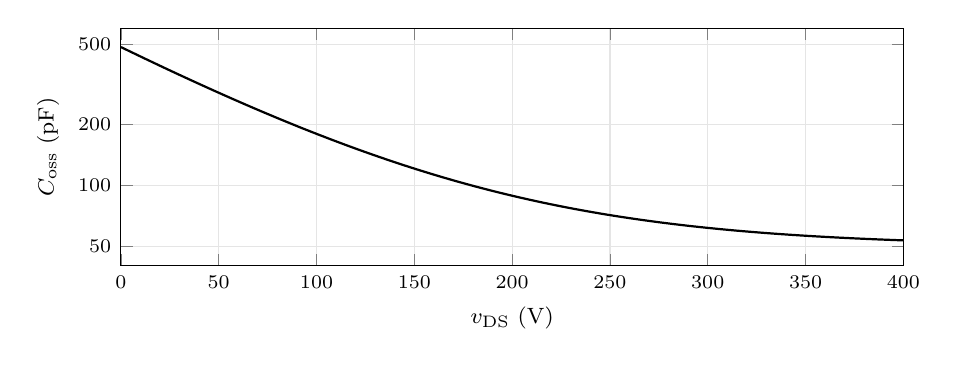
\begin{tikzpicture}
					\begin{semilogyaxis}[
							width=0.95\linewidth, height=4.6cm,
							xmin=0, xmax=400, ymin=40, ymax=600,
							xlabel={$v_\mathrm{DS}$ (V)}, ylabel={$C_\mathrm{oss}$ (pF)},
							ytick={50,100,200,500}, yticklabels={50,100,200,500},
							grid=major, grid style={gray!20},
							tick label style={font=\scriptsize}, label style={font=\footnotesize},
						]
						\addplot[black, thick, domain=0:400, samples=120] {50+434*exp(-x/83)};
					\end{semilogyaxis}
				\end{tikzpicture}
				\caption{Illustrative 650\,V GaN HEMT: $C_\mathrm{oss}=50\,\mathrm{pF}+434\,\mathrm{pF}\cdot e^{-v_\mathrm{DS}/83\,\mathrm{V}}$}
			\end{figure}
		\end{column}
		\begin{column}{0.47\textwidth}
			\begin{itemize}
				\item $C_\mathrm{oss}=C_\mathrm{DS}+C_\mathrm{GD}$ falls steeply at low voltage: by about one decade in GaN (the field plates deplete the 2DEG) and by two decades or more in Si superjunction MOSFETs (the pillars deplete).
				\item Charge and energy follow from the curve:
			\end{itemize}
			\begin{align*}
				Q_\mathrm{oss}(V) & = \int_0^V C_\mathrm{oss}(v)\,\mathrm{d}v \\
				E_\mathrm{oss}(V) & = \int_0^V v\,C_\mathrm{oss}(v)\,\mathrm{d}v
			\end{align*}
			For the model at 400\,V: $C_\mathrm{oss}=54$\,pF, $Q_\mathrm{oss}=55.7$\,nC, $E_\mathrm{oss}=6.9\,\mu$J.
		\end{column}
	\end{columns}
\end{frame}

%%%%%%%%%%%%%%%%%%%%%%%%%%%%%%%%%%%%%%%%%%%%%%%%%%%%%%%%%%%%%
%% Equivalent capacitances %%
%%%%%%%%%%%%%%%%%%%%%%%%%%%%%%%%%%%%%%%%%%%%%%%%%%%%%%%%%%%%%
\begin{frame}
	\frametitle{Equivalent output capacitances}
	Datasheets of high-voltage GaN, SiC and superjunction devices give two equivalent linear capacitances for charging from 0 to $V$ (e.g.\ 400\,V for 650\,V devices):
	\begin{table}
		\centering
		\small
		\begin{tabular}{|l|l|>{\raggedright\arraybackslash}p{5.4cm}|l|}
			\hline
			\textbf{Name}            & \textbf{Definition}                              & \textbf{Use}                                           & \textbf{Model, 400\,V} \\
			\hline
			time related $C_\mathrm{o(tr)}$   & $Q_\mathrm{oss}(V)/V$                  & charging time and charge: dead time, ZVS transition, hard turn-on loss & 139\,pF \\
			energy related $C_\mathrm{o(er)}$ & $2E_\mathrm{oss}(V)/V^2$               & stored energy                                          & 86\,pF \\
			small signal $C_\mathrm{oss}(V)$  & $\mathrm{d}Q_\mathrm{oss}/\mathrm{d}v$ at $V$ & resonance and ringing at the operating point     & 54\,pF \\
			\hline
		\end{tabular}
		\caption{Equivalent capacitances of the illustrative 650\,V device}
	\end{table}
	\begin{block}{Rule}
		For a $C_\mathrm{oss}(v)$ that falls with voltage, $C_\mathrm{oss}(V) < C_\mathrm{o(er)} < C_\mathrm{o(tr)}$. Using the small-signal value from the datasheet curve at the operating voltage underestimates both charge and energy.
	\end{block}
\end{frame}

%%%%%%%%%%%%%%%%%%%%%%%%%%%%%%%%%%%%%%%%%%%%%%%%%%%%%%%%%%%%%
%% Hard turn-on revisited %%
%%%%%%%%%%%%%%%%%%%%%%%%%%%%%%%%%%%%%%%%%%%%%%%%%%%%%%%%%%%%%
\begin{frame}
	\frametitle{Capacitive turn-on loss}
	\begin{columns}[T]
		\begin{column}{0.5\textwidth}
			\begin{figure}
				\centering
				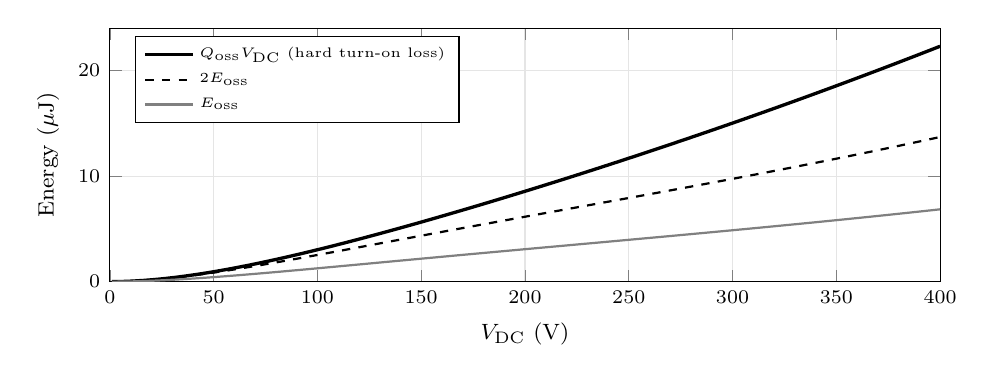
\begin{tikzpicture}
					\begin{axis}[
							width=\linewidth, height=4.8cm,
							xmin=0, xmax=400, ymin=0, ymax=24,
							xlabel={$V_\mathrm{DC}$ (V)}, ylabel={Energy ($\mu$J)},
							grid=major, grid style={gray!20},
							tick label style={font=\scriptsize}, label style={font=\footnotesize},
							legend style={font=\tiny}, legend pos=north west, legend cell align=left,
						]
						\addplot[black, very thick, domain=1:400, samples=80] {(50e-12*x+434e-12*83*(1-exp(-x/83)))*x*1e6};
						\addlegendentry{$Q_\mathrm{oss}V_\mathrm{DC}$ (hard turn-on loss)}
						\addplot[black, thick, dashed, domain=1:400, samples=80] {2*(25e-12*x^2+434e-12*83^2*(1-exp(-x/83)*(1+x/83)))*1e6};
						\addlegendentry{$2E_\mathrm{oss}$}
						\addplot[gray, thick, domain=1:400, samples=80] {(25e-12*x^2+434e-12*83^2*(1-exp(-x/83)*(1+x/83)))*1e6};
						\addlegendentry{$E_\mathrm{oss}$}
					\end{axis}
				\end{tikzpicture}
				\caption{Illustrative 650\,V GaN HEMT of the previous slides}
			\end{figure}
		\end{column}
		\begin{column}{0.47\textwidth}
			Hard turn-on in a half-bridge (Tutorial 1): $E=Q_\mathrm{oss}V_\mathrm{DC}$ for any shape of $C_\mathrm{oss}(v)$.\\[0.4em]
			Compared with the stored energy:
			\begin{equation*}
				Q_\mathrm{oss}V-2E_\mathrm{oss}=\int_0^V (V-2v)\,C_\mathrm{oss}(v)\,\mathrm{d}v \geq 0
			\end{equation*}
			if $C_\mathrm{oss}$ falls with $v$ (the weight $V-2v$ is positive where $C_\mathrm{oss}$ is large).\\[0.4em]
			At 400\,V: $Q_\mathrm{oss}V_\mathrm{DC}=22.3\,\mu$J, but $E_\mathrm{oss}=6.9\,\mu$J. An estimate based on $E_\mathrm{oss}$ is 3.3 times too optimistic.
		\end{column}
	\end{columns}
\end{frame}

%%%%%%%%%%%%%%%%%%%%%%%%%%%%%%%%%%%%%%%%%%%%%%%%%%%%%%%%%%%%%
%% Datasheet task %%
%%%%%%%%%%%%%%%%%%%%%%%%%%%%%%%%%%%%%%%%%%%%%%%%%%%%%%%%%%%%%
% Two pages: task (page 1) and task with solution (page 2).
\begin{frame}<handout:1-2>
	\frametitle{Reading a datasheet}
	\begin{columns}[T]
		\begin{column}{0.42\textwidth}
			\begin{table}
				\centering
				\small
				\begin{tabular}{|l|l|}
					\hline
					$R_\mathrm{DS(on)}$                & 5\,m$\Omega$     \\
					$Q_\mathrm{G}$ at 5\,V             & 7\,nC            \\
					$Q_\mathrm{GD}$                    & 1\,nC            \\
					$Q_\mathrm{oss}$ at 48\,V          & 25\,nC           \\
					$E_\mathrm{oss}$ at 48\,V          & 0.45\,$\mu$J     \\
					$V_\mathrm{SD}$ ($v_\mathrm{GS}=0$) & 1.8\,V          \\
					$Q_\mathrm{rr}$                    & 0                \\
					\hline
				\end{tabular}
				\caption{Illustrative 100\,V GaN transistor}
			\end{table}
		\end{column}
		\begin{column}{0.55\textwidth}
			\begin{block}{Task (5 minutes)}
				A half-bridge operates at 48\,V and 1\,MHz.
				\begin{enumerate}
					\item Calculate $C_\mathrm{o(tr)}$ and $C_\mathrm{o(er)}$.
					\item Capacitive loss with hard turn-on? What would an estimate with $E_\mathrm{oss}$ give?
					\item Minimum dead time for a ZVS transition driven by 10\,A and by 2\,A?
				\end{enumerate}
			\end{block}
		\end{column}
	\end{columns}
	\onslide<2-|handout:2>{
		\small
		\begin{enumerate}
			\item $C_\mathrm{o(tr)}=25\,\mathrm{nC}/48\,\mathrm{V}=521$\,pF, $C_\mathrm{o(er)}=2\cdot0.45\,\mu\mathrm{J}/(48\,\mathrm{V})^2=391$\,pF.
			\item $Q_\mathrm{oss}V_\mathrm{DC}f_\mathrm{sw}=1.2$\,W. With $E_\mathrm{oss}$: 0.45\,W, i.e.\ 2.7 times too low.
			\item The current moves the charge of both switches: $t_\mathrm{tr}=2Q_\mathrm{oss}/I$, i.e.\ 5\,ns at 10\,A and 25\,ns at 2\,A. A fixed dead time that works at full load is too short at light load (L8).
		\end{enumerate}
	}
\end{frame}

%%%%%%%%%%%%%%%%%%%%%%%%%%%%%%%%%%%%%%%%%%%%%%%%%%%%%%%%%%%%%
%% Coss hysteresis %%
%%%%%%%%%%%%%%%%%%%%%%%%%%%%%%%%%%%%%%%%%%%%%%%%%%%%%%%%%%%%%
\begin{frame}
	\frametitle{Output capacitance hysteresis}
	\begin{columns}[T]
		\begin{column}{0.42\textwidth}
			\begin{figure}
				\centering
				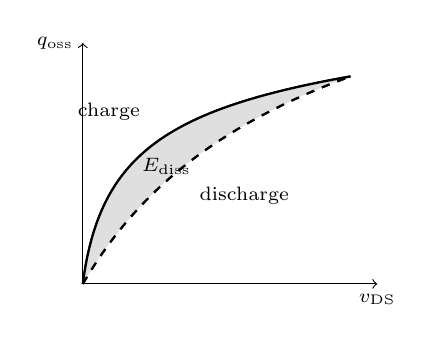
\begin{tikzpicture}[x=0.85cm, y=0.85cm, font=\scriptsize]
					\draw[->] (0,0) -- (4.4,0) node[below] {$v_\mathrm{DS}$};
					\draw[->] (0,0) -- (0,3.6) node[left] {$q_\mathrm{oss}$};
					% charging path (upper) and discharging path (lower)
					\draw[thick] (0,0) .. controls (0.25,1.9) and (1.2,2.6) .. (4,3.1);
					\draw[thick, dashed] (0,0) .. controls (0.7,1.2) and (1.8,2.3) .. (4,3.1);
					\fill[gray!25] (0,0) .. controls (0.25,1.9) and (1.2,2.6) .. (4,3.1) .. controls (1.8,2.3) and (0.7,1.2) .. (0,0);
					\draw[thick] (0,0) .. controls (0.25,1.9) and (1.2,2.6) .. (4,3.1);
					\draw[thick, dashed] (0,0) .. controls (0.7,1.2) and (1.8,2.3) .. (4,3.1);
					\node[anchor=south east] at (1.0,2.3) {charge};
					\node[anchor=north west] at (1.6,1.6) {discharge};
					\node at (1.25,1.75) {$E_\mathrm{diss}$};
				\end{tikzpicture}
				\caption{Measured charge--voltage loop (schematic); the enclosed area is the energy lost per cycle}
			\end{figure}
		\end{column}
		\begin{column}{0.55\textwidth}
			\small
			Soft switching is ideally lossless, but charging and discharging $C_\mathrm{oss}$ dissipates energy:
			\begin{itemize}
				\item reported for Si superjunction MOSFETs, GaN HEMTs and SiC diodes
				\item in GaN: equal to or greater than the conduction loss at MHz, rising exponentially with $\mathrm{d}v/\mathrm{d}t$
				\item a fixed fraction of $E_\mathrm{oss}$ is not a valid model: the loss depends on $f$, voltage swing and $\mathrm{d}v/\mathrm{d}t$
				\item within one device family the loss scales with $E_\mathrm{oss}$
			\end{itemize}
			Measured with Sawyer--Tower circuits (charge versus voltage) or calorimetrically (L5).
		\end{column}
	\end{columns}
	\blfootnote{Sources: Fedison et al., APEC 2014; Zulauf et al., IEEE TPEL, 2018; Perreault, APEC 2024 plenary.}
\end{frame}

%%%%%%%%%%%%%%%%%%%%%%%%%%%%%%%%%%%%%%%%%%%%%%%%%%%%%%%%%%%%%
%% Origin and size of Coss losses %%
%%%%%%%%%%%%%%%%%%%%%%%%%%%%%%%%%%%%%%%%%%%%%%%%%%%%%%%%%%%%%
\begin{frame}
	\frametitle{Origin and size of $C_\mathrm{oss}$ losses}
	\begin{columns}[T]
		\begin{column}{0.5\textwidth}
			\begin{figure}
				\centering
				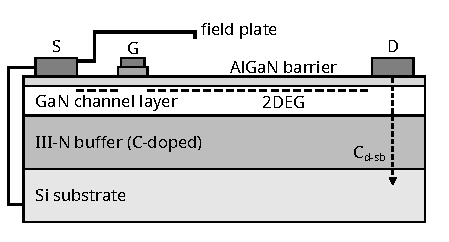
\includegraphics[width=0.92\linewidth]{fig/lec02/gan_on_si_hemt.pdf}
				\caption{Lateral GaN-on-Si HEMT (schematic, not to scale). In the device studied, up to 95\,\% of the loss came from $C_\mathrm{d\text{-}sb}$; an improved buffer cut the loss by about 70\,\%.}
			\end{figure}
		\end{column}
		\begin{column}{0.47\textwidth}
			\small
			Fit for one 650\,V GaN device (5--35\,MHz):
			\begin{equation*}
				E_\mathrm{diss}=k\,f^{\alpha}\,V_\mathrm{pp}^{\beta},\quad \alpha=0.6,\ \beta=1.7
			\end{equation*}
			\begin{table}
				\centering
				\footnotesize
				\begin{tabular}{|l|l|l|}
					\hline
					                & $E_\mathrm{diss}$ & $P=E_\mathrm{diss}f$ \\
					\hline
					10\,MHz, 400\,V & 0.12\,$\mu$J      & 1.2\,W               \\
					30\,MHz, 650\,V & 0.53\,$\mu$J      & 15.8\,W              \\
					\hline
				\end{tabular}
			\end{table}
			For comparison: 3\,A rms in 100\,m$\Omega$ give 0.9\,W. At tens of MHz, $C_\mathrm{oss}$ losses can dominate.
		\end{column}
	\end{columns}
	\blfootnote{Sources: Guacci et al., IEEE JESTPE, 2019; Zulauf et al., IEEE TPEL, 2018 (GS66504B, $k=2.84\cdot10^{-10}$, $E$ in $\mu$J).}
\end{frame}

%%%%%%%%%%%%%%%%%%%%%%%%%%%%%%%%%%%%%%%%%%%%%%%%%%%%%%%%%%%%%
%% Loss inventory %%
%%%%%%%%%%%%%%%%%%%%%%%%%%%%%%%%%%%%%%%%%%%%%%%%%%%%%%%%%%%%%
\subsection{Loss inventory at MHz}

\begin{frame}
	\frametitle{Conduction loss at MHz}
	$P_\mathrm{cond}=I_\mathrm{rms}^2\,\big(R_\mathrm{DS(on)}(T_\mathrm{j},t)+R_\mathrm{ac}(f)\big)$, with $R_\mathrm{ac}$ of package and PCB.
	\begin{itemize}
		\item $R_\mathrm{DS(on)}$ typically rises by a factor of 1.5 to 2.5 from 25\,$^\circ$C to 150\,$^\circ$C. Use the datasheet curve at the expected junction temperature.
		\item GaN HEMTs show a dynamic $R_\mathrm{DS(on)}$ (next slide).
		\item Leads and traces have skin and proximity effect at MHz (L3, L7).
		\item Soft-switching schemes often need a larger RMS current.
	\end{itemize}
	\begin{block}{Example: triangular current mode}
		A buck converter with 10\,A output current needs an inductor current between $-2$\,A and 22\,A for ZVS (L8):
		\begin{equation*}
			I_\mathrm{rms}=\sqrt{I_\mathrm{avg}^2+\Delta I^2/12}=\sqrt{10^2+24^2/12}\,\mathrm{A}=12.2\,\mathrm{A}
		\end{equation*}
		The conduction loss is 48\,\% higher than with a small ripple.
	\end{block}
\end{frame}

%%%%%%%%%%%%%%%%%%%%%%%%%%%%%%%%%%%%%%%%%%%%%%%%%%%%%%%%%%%%%
%% Dynamic Ron %%
%%%%%%%%%%%%%%%%%%%%%%%%%%%%%%%%%%%%%%%%%%%%%%%%%%%%%%%%%%%%%
\begin{frame}
	\frametitle{Dynamic on-resistance of GaN}
	\begin{columns}[T]
		\begin{column}{0.42\textwidth}
			\begin{figure}
				\centering
				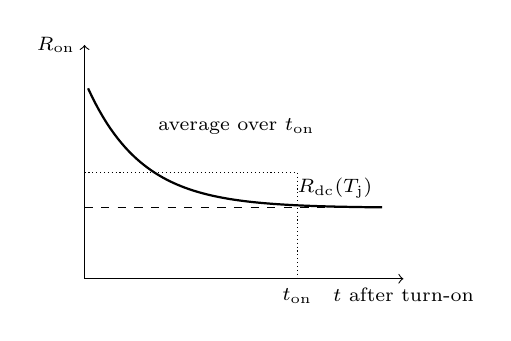
\begin{tikzpicture}[x=0.9cm, y=0.9cm, font=\scriptsize]
					\draw[->] (0,0) -- (4.5,0) node[below] {$t$ after turn-on};
					\draw[->] (0,0) -- (0,3.3) node[left] {$R_\mathrm{on}$};
					\draw[dashed] (0,1) -- (4.2,1) node[above left] {$R_\mathrm{dc}(T_\mathrm{j})$};
					\draw[thick, domain=0.05:4.2, samples=80] plot (\x, {1+1.8*exp(-1.3*\x)});
					\draw[densely dotted] (0,1.5) -- (3,1.5) -- (3,0);
					\node[anchor=north] at (3,0) {$t_\mathrm{on}$};
					\node[anchor=south west] at (0.9,1.9) {average over $t_\mathrm{on}$};
				\end{tikzpicture}
				\caption{Dynamic on-resistance after turn-on (schematic)}
			\end{figure}
		\end{column}
		\begin{column}{0.55\textwidth}
			\small
			Electrons trapped in the buffer, in the channel layer or at the surface reduce the 2DEG density for some time after turn-on.
			\begin{itemize}
				\item \textbf{Off-state trapping} grows with blocking voltage and blocking time.
				\item \textbf{Hot-electron trapping} occurs during hard turn-on. To first order it is absent with soft switching.
				\item Traps accumulate over many cycles. A double-pulse test therefore underestimates the effect; measure in continuous operation (L5).
			\end{itemize}
			Published values for 600/650\,V devices range from negligible to five to eight times $R_\mathrm{dc}$. For the device measured by Zulauf et al.\ the worst case was about $2R_\mathrm{dc}$.
		\end{column}
	\end{columns}
	\blfootnote{Source: Zulauf, Guacci, Kolar, IEEE TPEL, vol. 35, no. 6, 2020.}
\end{frame}

%%%%%%%%%%%%%%%%%%%%%%%%%%%%%%%%%%%%%%%%%%%%%%%%%%%%%%%%%%%%%
%% Turn-off with capacitive snubbing %%
%%%%%%%%%%%%%%%%%%%%%%%%%%%%%%%%%%%%%%%%%%%%%%%%%%%%%%%%%%%%%
\begin{frame}
	\frametitle{Turn-off with output capacitance}
	\begin{columns}[T]
		\begin{column}{0.45\textwidth}
			\begin{figure}
				\centering
				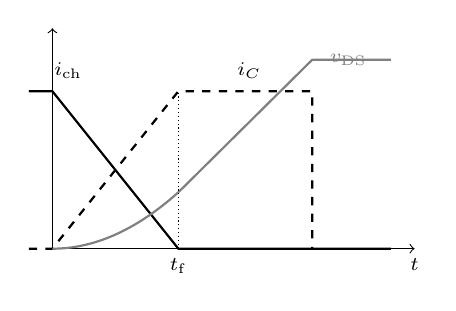
\begin{tikzpicture}[x=1.0cm, y=0.8cm, font=\scriptsize]
					\draw[->] (0,0) -- (4.6,0) node[below] {$t$};
					\draw[->] (0,0) -- (0,3.5);
					% channel current falls linearly within t_f
					\draw[thick] (-0.3,2.5) -- (0,2.5) -- (1.6,0) -- (4.3,0);
					\node[anchor=south] at (0.2,2.55) {$i_\mathrm{ch}$};
					% capacitor current rises to I
					\draw[thick, dashed] (-0.3,0) -- (0,0) -- (1.6,2.5) -- (3.3,2.5) -- (3.3,0);
					\node[anchor=south] at (2.5,2.55) {$i_C$};
					% voltage: parabola during t_f, then linear
					\draw[thick, gray, domain=0:1.6, samples=40] plot (\x, {0.35*\x*\x});
					\draw[thick, gray] (1.6,0.896) -- (3.3,3.0) -- (4.3,3.0);
					\node[anchor=west, gray] at (3.4,3.0) {$v_\mathrm{DS}$};
					\draw[densely dotted] (1.6,0) -- (1.6,2.5);
					\node[anchor=north] at (1.6,0) {$t_\mathrm{f}$};
				\end{tikzpicture}
				\caption{Turn-off of a constant current $I$ with a capacitance $C$ across the switch node}
			\end{figure}
		\end{column}
		\begin{column}{0.52\textwidth}
			If the channel current falls linearly within $t_\mathrm{f}$, the rest of the current charges $C$ and the voltage rises slowly:
			\begin{equation*}
				E_\mathrm{off}=\int_0^{t_\mathrm{f}} v_\mathrm{DS}\,i_\mathrm{ch}\,\mathrm{d}t=\frac{I^2t_\mathrm{f}^2}{24\,C}
				\quad\text{for}\quad \frac{I\,t_\mathrm{f}}{2C}<V_\mathrm{DC}
			\end{equation*}
			$C$ is the total switch-node capacitance (both $C_\mathrm{oss}$ and parasitics).\\[0.4em]
			Example: $I=10$\,A, $t_\mathrm{f}=2$\,ns, $C=400$\,pF gives 42\,nJ, compared with $\frac12 V_\mathrm{DC}It_\mathrm{f}=480$\,nJ at 48\,V.
			\begin{block}{Key message}
				A fast channel turn-off is almost lossless. Extra capacitance helps the turn-off but increases the loss of a hard turn-on.
			\end{block}
		\end{column}
	\end{columns}
\end{frame}

%%%%%%%%%%%%%%%%%%%%%%%%%%%%%%%%%%%%%%%%%%%%%%%%%%%%%%%%%%%%%
%% Reverse conduction and recovery %%
%%%%%%%%%%%%%%%%%%%%%%%%%%%%%%%%%%%%%%%%%%%%%%%%%%%%%%%%%%%%%
\begin{frame}
	\frametitle{Reverse conduction and recovery}
	\begin{table}
		\centering
		\footnotesize
		\begin{tabular}{|l|>{\raggedright\arraybackslash}p{3.4cm}|>{\raggedright\arraybackslash}p{4.0cm}|>{\raggedright\arraybackslash}p{3.2cm}|}
			\hline
			                   & \textbf{Si MOSFET}             & \textbf{e-mode GaN HEMT}                                          & \textbf{SiC MOSFET}          \\
			\hline
			Reverse path       & p--n body diode                & channel, opened by $v_\mathrm{GD}>V_\mathrm{th}$                  & p--n body diode              \\
			$V_\mathrm{SD}$    & about 0.7--1\,V                & about 1.5--3\,V (current dependent), plus $|v_\mathrm{GS,off}|$ for negative gate bias & about 3\,V or more (SiC junction) \\
			Recovery charge    & large (minority carriers)      & none                                                              & small                        \\
			\hline
		\end{tabular}
		\caption{Third-quadrant conduction during the dead time}
	\end{table}
	\begin{itemize}
		\item Datasheets: 100\,V Si MOSFET (6\,m$\Omega$) $Q_\mathrm{rr}=109$\,nC at 100\,A/$\mu$s; 100\,V GaN (7\,m$\Omega$) $V_\mathrm{SD}=1.7$\,V at 0.5\,A, no $Q_\mathrm{rr}$.
		\item $V_\mathrm{SD}$ of GaN rises by 1\,V for $v_\mathrm{GS,off}=-1$\,V and rises with temperature.
		\item Hard turn-on against a recovering Si diode costs about $Q_\mathrm{rr}V_\mathrm{DC}$; $Q_\mathrm{rr}$ grows with $\mathrm{d}i/\mathrm{d}t$ and temperature.
	\end{itemize}
	\blfootnote{Source: Lidow et al., GaN Transistors for Efficient Power Conversion, 3rd ed., 2019, Sec. 2.6 (EPC2045, BSC060N10NS3\,G).}
\end{frame}

%%%%%%%%%%%%%%%%%%%%%%%%%%%%%%%%%%%%%%%%%%%%%%%%%%%%%%%%%%%%%
%% Your turn: dead-time loss %%
%%%%%%%%%%%%%%%%%%%%%%%%%%%%%%%%%%%%%%%%%%%%%%%%%%%%%%%%%%%%%
% Two pages: task (page 1) and task with solution (page 2).
\begin{frame}<handout:1-2>
	\frametitle{Dead-time loss}
	\begin{block}{Task (3 minutes)}
		A GaN half-bridge switches 10\,A at 2\,MHz. During each of the two dead times per period ($t_\mathrm{d}=10$\,ns) the current flows in reverse through the GaN channel with $V_\mathrm{SD}=2.5$\,V.
		\begin{enumerate}
			\item Calculate the dead-time loss.
			\item How can it be reduced?
		\end{enumerate}
	\end{block}
	\onslide<2-|handout:2>{
		\begin{enumerate}
			\item $P_\mathrm{dt}=2\,V_\mathrm{SD}\,I\,t_\mathrm{d}\,f_\mathrm{sw}=2\cdot2.5\,\mathrm{V}\cdot10\,\mathrm{A}\cdot10\,\mathrm{ns}\cdot2\,\mathrm{MHz}=1$\,W.
			\item \begin{itemize}
				      \item Make the dead time only as long as the voltage transition, $2Q_\mathrm{oss}/I$ (adaptive dead time, L4).
				      \item Turn the GaN transistor off with 0\,V instead of a negative voltage, if the gate loop allows it.
				      \item A parallel Schottky diode lowers $V_\mathrm{SD}$, but adds its capacitance to the switch node.
			      \end{itemize}
		\end{enumerate}
	}
\end{frame}

%%%%%%%%%%%%%%%%%%%%%%%%%%%%%%%%%%%%%%%%%%%%%%%%%%%%%%%%%%%%%
%% Gate-drive loss %%
%%%%%%%%%%%%%%%%%%%%%%%%%%%%%%%%%%%%%%%%%%%%%%%%%%%%%%%%%%%%%
\begin{frame}
	\frametitle{Gate-drive loss}
	\begin{columns}[T]
		\begin{column}{0.45\textwidth}
			\begin{figure}
				\centering
				\begin{circuitikz}[scale=0.8, transform shape]
					\draw (0,0) to[V, l=$V_\mathrm{dr}$] (0,2.4) to[R, l=$R_\mathrm{dr}$] (2.2,2.4) to[R, l=$R_\mathrm{G,ext}$] (4.4,2.4) to[R, l=$R_\mathrm{G,int}$] (4.4,0.9) to[C, l=$C_\mathrm{iss}$] (4.4,-0.6) -- (4.4,-0.6) -- (0,-0.6) -- (0,0);
				\end{circuitikz}
				\caption{Gate loop: driver output resistance, external and internal gate resistance}
			\end{figure}
		\end{column}
		\begin{column}{0.52\textwidth}
			Charging and discharging the gate draws $P_\mathrm{G}=Q_\mathrm{G}\,V_\mathrm{dr}\,f_\mathrm{sw}$ per switch from the driver supply. It is dissipated in $R_\mathrm{dr}$, $R_\mathrm{G,ext}$ and $R_\mathrm{G,int}$ in proportion to their values; the total does not depend on $R_\mathrm{G}$.
			\begin{itemize}
				\item Use $Q_\mathrm{G}$ at $V_\mathrm{dr}$ from the gate-charge curve.
				\item 100\,V GaN, 7\,nC at 5\,V: 0.35\,W per switch at 10\,MHz.
				\item 100\,V Si, 35\,nC at 10\,V: 0.35\,W per switch at 1\,MHz.
				\item Driver quiescent and level-shifter losses also grow with $f_\mathrm{sw}$. Resonant gate drivers recover part of the energy (L4).
			\end{itemize}
		\end{column}
	\end{columns}
\end{frame}

%%%%%%%%%%%%%%%%%%%%%%%%%%%%%%%%%%%%%%%%%%%%%%%%%%%%%%%%%%%%%
%% Si versus GaN at 48 V %%
%%%%%%%%%%%%%%%%%%%%%%%%%%%%%%%%%%%%%%%%%%%%%%%%%%%%%%%%%%%%%
\begin{frame}
	\frametitle{Silicon versus GaN at 48\,V}
	\begin{columns}[T]
		\begin{column}{0.52\textwidth}
			\begin{figure}
				\centering
				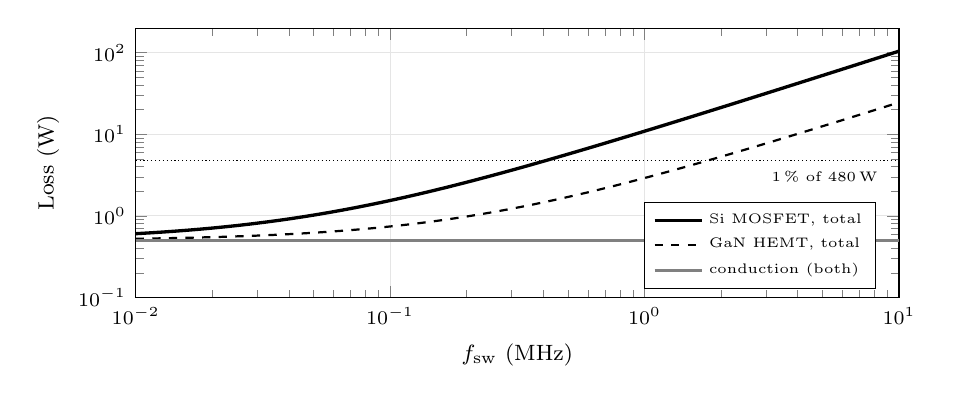
\begin{tikzpicture}
					\begin{loglogaxis}[
							width=0.93\linewidth, height=5.0cm,
							xmin=0.01, xmax=10, ymin=0.1, ymax=200,
							xlabel={$f_\mathrm{sw}$ (MHz)}, ylabel={Loss (W)},
							grid=major, grid style={gray!20},
							tick label style={font=\scriptsize}, label style={font=\footnotesize},
							legend style={font=\tiny}, legend pos=south east, legend cell align=left,
						]
						\addplot[black, very thick, domain=-2:1, samples=60] ({10^x}, {0.5+10.42*10^x});
						\addlegendentry{Si MOSFET, total}
						\addplot[black, thick, dashed, domain=-2:1, samples=60] ({10^x}, {0.5+2.41*10^x});
						\addlegendentry{GaN HEMT, total}
						\addplot[gray, thick, domain=-2:1, samples=2] ({10^x}, {0.5});
						\addlegendentry{conduction (both)}
						\addplot[black, densely dotted, domain=-2:1, samples=2, forget plot] ({10^x}, {4.8});
						\node[font=\tiny, anchor=north east] at (axis cs:9,4.6) {1\,\% of 480\,W};
					\end{loglogaxis}
				\end{tikzpicture}
				\caption{Hard-switched half-bridge, 48\,V, 10\,A, illustrative device values}
			\end{figure}
		\end{column}
		\begin{column}{0.45\textwidth}
			\footnotesize
			\begin{tabular}{|l|r|r|}
				\hline
				Energy per period ($\mu$J)                & Si    & GaN  \\
				\hline
				$Q_\mathrm{oss}V_\mathrm{DC}$             & 2.88  & 1.20 \\
				$V$--$I$ overlap                          & 3.60  & 0.96 \\
				$Q_\mathrm{rr}V_\mathrm{DC}$              & 2.88  & 0    \\
				dead time                                 & 0.36  & 0.18 \\
				gate, two switches                        & 0.70  & 0.07 \\
				\hline
				sum                                       & 10.42 & 2.41 \\
				\hline
			\end{tabular}\\[0.5em]
			Assumed: $R_\mathrm{DS(on)}=5$\,m$\Omega$ for both. Si: $Q_\mathrm{oss}=60$\,nC, $t_\mathrm{r}+t_\mathrm{f}=15$\,ns, $Q_\mathrm{rr}=60$\,nC, $Q_\mathrm{G}=35$\,nC at 10\,V, $t_\mathrm{d}=20$\,ns. GaN: values of the datasheet task, $t_\mathrm{r}+t_\mathrm{f}=4$\,ns, $t_\mathrm{d}=5$\,ns.\\[0.5em]
			Switching loss equals conduction loss at 48\,kHz (Si) and 210\,kHz (GaN). The total loss reaches 1\,\% of the output power at 0.41\,MHz and 1.8\,MHz.
		\end{column}
	\end{columns}
\end{frame}

%%%%%%%%%%%%%%%%%%%%%%%%%%%%%%%%%%%%%%%%%%%%%%%%%%%%%%%%%%%%%
%% Poll: dominant loss %%
%%%%%%%%%%%%%%%%%%%%%%%%%%%%%%%%%%%%%%%%%%%%%%%%%%%%%%%%%%%%%
% Two pages: question (page 1) and answer (page 2).
\begin{frame}<handout:1-2>
	\frametitle{Dominant loss at 5\,MHz}
	The GaN half-bridge of the previous slide is hard switched at 5\,MHz. Which loss is the largest? Vote and justify in one sentence.
	\begin{enumerate}[(a)]
		\item conduction
		\item gate drive
		\item $Q_\mathrm{oss}V_\mathrm{DC}$
		\item $V$--$I$ overlap
		\item dead time
	\end{enumerate}
	\onslide<2-|handout:2>{
		\begin{block}{Answer: (c)}
			At 5\,MHz: $Q_\mathrm{oss}V_\mathrm{DC}$ 6.0\,W, overlap 4.8\,W, dead time 0.9\,W, conduction 0.5\,W, gate 0.35\,W; total 12.6\,W or 2.6\,\% of 480\,W. A stronger gate driver only reduces the overlap term. The capacitive term requires zero-voltage switching.
		\end{block}
	}
\end{frame}

%%%%%%%%%%%%%%%%%%%%%%%%%%%%%%%%%%%%%%%%%%%%%%%%%%%%%%%%%%%%%
%% Hard versus soft switching %%
%%%%%%%%%%%%%%%%%%%%%%%%%%%%%%%%%%%%%%%%%%%%%%%%%%%%%%%%%%%%%
\subsection{Hard versus soft switching}

\begin{frame}
	\frametitle{Soft-switching techniques}
	\begin{table}
		\centering
		\small
		\begin{tabular}{|>{\raggedright\arraybackslash}p{2.9cm}|>{\raggedright\arraybackslash}p{4.4cm}|>{\raggedright\arraybackslash}p{4.9cm}|}
			\hline
			\textbf{Technique}                    & \textbf{Removes}                                                          & \textbf{Remains}                                                                    \\
			\hline
			Zero-voltage switching (ZVS) at turn-on & $Q_\mathrm{oss}V_\mathrm{DC}$, turn-on overlap, reverse recovery          & turn-off overlap (small with $C_\mathrm{oss}$), $C_\mathrm{oss}$ hysteresis, gate drive, dead-time conduction, larger RMS current \\
			\hline
			Zero-current switching (ZCS) at turn-off & turn-off overlap, tail current (IGBT)                                    & $Q_\mathrm{oss}V_\mathrm{DC}$ at turn-on, unless the voltage is also zero              \\
			\hline
			Auxiliary circuits (ZVT, ZCT)         & as ZVS or ZCS for the main switch                                         & losses and complexity of the auxiliary switch                                       \\
			\hline
		\end{tabular}
		\caption{Which loss terms are removed by soft switching}
	\end{table}
	\begin{itemize}
		\item MOSFETs and GaN HEMTs need ZVS: their main loss is the capacitive turn-on loss, which ZCS does not remove.
		\item ZVS needs an inductive current that commutates the switch node within the dead time (L8--L10).
	\end{itemize}
\end{frame}

%%%%%%%%%%%%%%%%%%%%%%%%%%%%%%%%%%%%%%%%%%%%%%%%%%%%%%%%%%%%%
%% Poll: larger die %%
%%%%%%%%%%%%%%%%%%%%%%%%%%%%%%%%%%%%%%%%%%%%%%%%%%%%%%%%%%%%%
% Two pages: question (page 1) and answer (page 2).
\begin{frame}<handout:1-2>
	\frametitle{Larger die, lower loss?}
	You replace the GaN transistor of the 48\,V half-bridge by one with twice the die area, i.e.\ half the $R_\mathrm{DS(on)}$ and twice all charges. Does the loss go down? Vote: yes, no, it depends.
	\onslide<2-|handout:2>{
		\begin{block}{Answer: it depends on $f_\mathrm{sw}$}
			Conduction loss halves, all charge-related losses double:
			\begin{itemize}
				\item 100\,kHz: $0.5+0.24\,\mathrm{W}\rightarrow 0.25+0.48\,\mathrm{W}$, practically no change.
				\item 1\,MHz: $0.5+2.41\,\mathrm{W}\rightarrow 0.25+4.82\,\mathrm{W}$, the loss rises by 74\,\%.
			\end{itemize}
			Above a certain frequency a smaller die is better. The next slide finds the optimum.
		\end{block}
	}
\end{frame}

%%%%%%%%%%%%%%%%%%%%%%%%%%%%%%%%%%%%%%%%%%%%%%%%%%%%%%%%%%%%%
%% Optimum die size %%
%%%%%%%%%%%%%%%%%%%%%%%%%%%%%%%%%%%%%%%%%%%%%%%%%%%%%%%%%%%%%
\begin{frame}
	\frametitle{Optimum die size}
	\begin{columns}[T]
		\begin{column}{0.5\textwidth}
			\begin{figure}
				\centering
				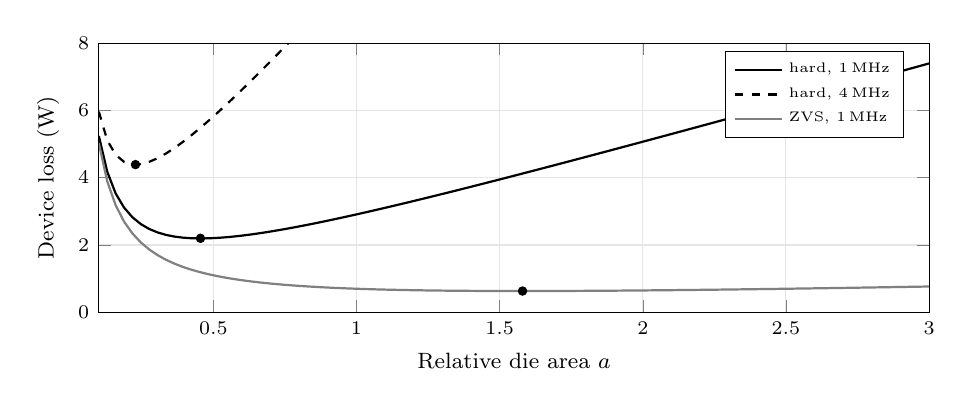
\begin{tikzpicture}
					\begin{axis}[
							width=\linewidth, height=5.0cm,
							xmin=0.1, xmax=3, ymin=0, ymax=8,
							xlabel={Relative die area $a$}, ylabel={Device loss (W)},
							grid=major, grid style={gray!20},
							tick label style={font=\scriptsize}, label style={font=\footnotesize},
							legend style={font=\tiny}, legend pos=north east, legend cell align=left,
						]
						\addplot[black, thick, domain=0.1:3, samples=100] {0.5/x+2.41*x};
						\addlegendentry{hard, 1\,MHz}
						\addplot[black, thick, dashed, domain=0.1:3, samples=100] {0.5/x+2.41*4*x};
						\addlegendentry{hard, 4\,MHz}
						\addplot[gray, thick, domain=0.1:3, samples=100] {0.5/x+0.2*x};
						\addlegendentry{ZVS, 1\,MHz}
						\addplot[only marks, mark=*, mark size=1.5pt, forget plot] coordinates {(0.455,2.20) (0.228,4.39) (1.58,0.632)};
					\end{axis}
				\end{tikzpicture}
				\caption{48\,V, 10\,A half-bridge; $a=1$ is the GaN device of the previous slides; ZVS: 0.2\,$\mu$J per period remain}
			\end{figure}
		\end{column}
		\begin{column}{0.47\textwidth}
			\small With die area $a$: $R_\mathrm{DS(on)}=R_1/a$, energy per period $E_1\,a$:
			\begin{gather*}
				P(a)=\frac{I_\mathrm{rms}^2R_1}{a}+E_1\,a\,f_\mathrm{sw}\\
				a_\mathrm{opt}=I_\mathrm{rms}\sqrt{R_1/(E_1f_\mathrm{sw})}\\
				P_\mathrm{min}=2I_\mathrm{rms}\sqrt{R_1E_1f_\mathrm{sw}}
			\end{gather*}
			\begin{itemize}
				\item At the optimum, conduction loss equals switching loss.
				\item $P_\mathrm{min}\propto\sqrt{f_\mathrm{sw}}$ and $\propto\sqrt{R_1E_1}$, the root of a figure of merit.
				\item Soft switching lowers $E_1$: larger die, lower loss.
			\end{itemize}
		\end{column}
	\end{columns}
\end{frame}

%%%%%%%%%%%%%%%%%%%%%%%%%%%%%%%%%%%%%%%%%%%%%%%%%%%%%%%%%%%%%
%% Devices %%
%%%%%%%%%%%%%%%%%%%%%%%%%%%%%%%%%%%%%%%%%%%%%%%%%%%%%%%%%%%%%
\subsection{Devices for high frequency}

\begin{frame}
	\frametitle{Devices up to 100\,V}
	\begin{table}
		\centering
		\small
		\begin{tabular}{|l|>{\raggedright\arraybackslash}p{4.9cm}|>{\raggedright\arraybackslash}p{5.5cm}|}
			\hline
			                       & \textbf{Si trench / shielded-gate MOSFET}        & \textbf{e-mode GaN HEMT}                              \\
			\hline
			Structure              & vertical                                         & lateral, all contacts on top                          \\
			Gate drive             & 10\,V, robust ($\pm20$\,V)                       & 5\,V, absolute maximum about $+6/-4$\,V                \\
			Charges per $R_\mathrm{DS(on)}$ & reference                               & several times lower $Q_\mathrm{G}$, $Q_\mathrm{GD}$, $Q_\mathrm{oss}$ \\
			Reverse recovery       & yes                                              & none                                                  \\
			Package                & QFN, power stages with driver                    & chip-scale LGA/BGA, package inductance of a few hundred pH \\
			\hline
		\end{tabular}
		\caption{Low-voltage device technologies}
	\end{table}
	\begin{itemize}
		\item Trend to integration: Si power stages, monolithic GaN power ICs.
		\item At 48\,V and several MHz GaN is the usual choice; at 12\,V below 1\,MHz Si power stages remain competitive.
	\end{itemize}
	\blfootnote{Sources: Lidow et al., 2019; Reusch and Strydom, IEEE TPEL, 2014.}
\end{frame}

%%%%%%%%%%%%%%%%%%%%%%%%%%%%%%%%%%%%%%%%%%%%%%%%%%%%%%%%%%%%%
%% High-voltage devices %%
%%%%%%%%%%%%%%%%%%%%%%%%%%%%%%%%%%%%%%%%%%%%%%%%%%%%%%%%%%%%%
\begin{frame}
	\frametitle{Devices for 600--650\,V}
	\begin{table}
		\centering
		\small
		\begin{tabular}{|l|>{\raggedright\arraybackslash}p{9.6cm}|}
			\hline
			Si superjunction MOSFET & cheap and robust, but large $Q_\mathrm{rr}$, strongly nonlinear $C_\mathrm{oss}$ with large $Q_\mathrm{oss}$ and hysteresis; mainly below a few hundred kHz \\
			e-mode GaN (p-GaN gate) & lowest charges, no $Q_\mathrm{rr}$; sensitive gate (low $V_\mathrm{th}$, limited gate voltage), dynamic $R_\mathrm{DS(on)}$, $C_\mathrm{oss}$ losses at MHz \\
			Cascode GaN             & normally-on GaN with a low-voltage Si MOSFET, robust gate; the Si MOSFET adds charge and a recovery effect \\
			SiC MOSFET              & high temperature capability and avalanche robustness; larger charges and 15--18\,V gate drive; body diode with high $V_\mathrm{SD}$ \\
			\hline
		\end{tabular}
		\caption{High-voltage device technologies for switching at hundreds of kHz to MHz}
	\end{table}
	\begin{itemize}
		\item The $C_\mathrm{oss}$ loss ranking depends on the voltage swing: in one study the cascode device had lower losses below 300\,V, the e-mode devices above.
		\item Choose by voltage, switching mode (hard or soft) and frequency, then compare complete loss budgets (Tutorial 2).
	\end{itemize}
	\blfootnote{Source: Zulauf et al., IEEE TPEL, vol. 33, no. 12, 2018.}
\end{frame}

%%%%%%%%%%%%%%%%%%%%%%%%%%%%%%%%%%%%%%%%%%%%%%%%%%%%%%%%%%%%%
%% Common-source inductance %%
%%%%%%%%%%%%%%%%%%%%%%%%%%%%%%%%%%%%%%%%%%%%%%%%%%%%%%%%%%%%%
\begin{frame}
	\frametitle{Common-source inductance}
	\begin{columns}[T]
		\begin{column}{0.48\textwidth}
			\begin{figure}
				\centering
				\begin{circuitikz}[scale=0.8, transform shape]
					\draw (3,2) node[nigfete](T){};
					\draw (T.D) -- ++(0,0.6) node[above] {drain};
					\draw (T.S) to[L, l_=$L_\mathrm{CS}$] (3,-0.6) coordinate (s) -- ++(0,-0.4) node[below] {power source};
					\draw (T.G) -- ++(-0.4,0) coordinate (g) to[R, l_=$R_\mathrm{G}$] ($(g)+(-1.6,0)$) coordinate (d) to[sV, l_=driver] (d |- s) -- (s);
					\draw (s) node[circ]{};
					\draw[->] (3.5,1.5) -- (3.5,0.3) node[midway, right] {$i_\mathrm{D}$};
				\end{circuitikz}
				\caption{The inductance $L_\mathrm{CS}$ is common to the power loop and the gate loop}
			\end{figure}
		\end{column}
		\begin{column}{0.49\textwidth}
			\small
			During the current transitions $L_\mathrm{CS}$ induces a voltage that opposes the gate drive:
			\begin{equation*}
				v_\mathrm{GS}=v_\mathrm{dr}-R_\mathrm{G}i_\mathrm{G}-L_\mathrm{CS}\frac{\mathrm{d}i_\mathrm{D}}{\mathrm{d}t}
			\end{equation*}
			1\,nH at 5\,A/ns gives 5\,V, as much as the whole GaN gate drive voltage.
			\begin{itemize}
				\item slower current transitions, more overlap loss
				\item calculated for a GaN buck: 1\,nH of $L_\mathrm{CS}$ adds 50\,\% loss (Reusch and Strydom)
				\item remedy: Kelvin-source pin for the gate loop, low-inductance package
			\end{itemize}
		\end{column}
	\end{columns}
	\blfootnote{Sources: Lidow et al., 2019, Sec. 3.6.1 and 7.3.1; Reusch and Strydom, IEEE TPEL, vol. 29, no. 4, 2014.}
\end{frame}

%%%%%%%%%%%%%%%%%%%%%%%%%%%%%%%%%%%%%%%%%%%%%%%%%%%%%%%%%%%%%
%% Datasheet limits %%
%%%%%%%%%%%%%%%%%%%%%%%%%%%%%%%%%%%%%%%%%%%%%%%%%%%%%%%%%%%%%
\begin{frame}
	\frametitle{What datasheets do not show}
	\begin{columns}[T]
		\begin{column}{0.48\textwidth}
			\textbf{Usually given}
			\begin{itemize}
				\item $R_\mathrm{DS(on)}$ versus temperature
				\item $Q_\mathrm{G}$, $Q_\mathrm{GS}$, $Q_\mathrm{GD}$ and the gate-charge curve
				\item $C_\mathrm{oss}(v)$, $Q_\mathrm{oss}$, $E_\mathrm{oss}$, $C_\mathrm{o(tr)}$, $C_\mathrm{o(er)}$
				\item $V_\mathrm{SD}$ and $Q_\mathrm{rr}$ at one operating point
				\item $E_\mathrm{on}$, $E_\mathrm{off}$ from a double-pulse test on the manufacturer's board
			\end{itemize}
		\end{column}
		\begin{column}{0.48\textwidth}
			\textbf{Usually missing}
			\begin{itemize}
				\item $C_\mathrm{oss}$ hysteresis loss under soft switching
				\item dynamic $R_\mathrm{DS(on)}$ in continuous operation
				\item $Q_\mathrm{rr}$ at your $\mathrm{d}i/\mathrm{d}t$ and temperature
				\item switching energies with your layout, gate driver and loop inductance
			\end{itemize}
		\end{column}
	\end{columns}
	\begin{block}{Consequence}
		A loss budget from datasheet values is a first estimate. The missing terms must be measured in the application, which is the subject of L5.
	\end{block}
\end{frame}

%%%%%%%%%%%%%%%%%%%%%%%%%%%%%%%%%%%%%%%%%%%%%%%%%%%%%%%%%%%%%
%% Key messages %%
%%%%%%%%%%%%%%%%%%%%%%%%%%%%%%%%%%%%%%%%%%%%%%%%%%%%%%%%%%%%%
\begin{frame}
	\frametitle{Key messages}
	\begin{enumerate}
		\item The hard turn-on loss is $Q_\mathrm{oss}V_\mathrm{DC}$. Estimates with $E_\mathrm{oss}$ or with the small-signal $C_\mathrm{oss}$ are too optimistic.
		\item Use $C_\mathrm{o(tr)}$ for charge and time, $C_\mathrm{o(er)}$ for stored energy.
		\item Soft switching removes the capacitive turn-on loss, but $C_\mathrm{oss}$ hysteresis, gate drive, dead time and a larger RMS current remain.
		\item At the optimum die size, conduction and switching loss are equal and the total loss grows with $\sqrt{f_\mathrm{sw}}$.
		\item Low common-source and package inductance are as important as the device itself.
	\end{enumerate}
\end{frame}

%%%%%%%%%%%%%%%%%%%%%%%%%%%%%%%%%%%%%%%%%%%%%%%%%%%%%%%%%%%%%
%% Exit ticket %%
%%%%%%%%%%%%%%%%%%%%%%%%%%%%%%%%%%%%%%%%%%%%%%%%%%%%%%%%%%%%%
% Two pages: questions (page 1) and answers (page 2).
\begin{frame}<handout:1-2>
	\frametitle{Exit ticket}
	\begin{varblock}[\textwidth]{Three questions, one minute each}
		\begin{enumerate}
			\item Which equivalent capacitance gives the time of a ZVS transition?
			\item Name two losses that remain in a GaN half-bridge with perfect ZVS.
			\item The switching frequency of an optimally sized design rises from 1 to 4\,MHz. By which factor does the minimum device loss change?
		\end{enumerate}
	\end{varblock}
	\onslide<2-|handout:2>{
		\begin{enumerate}
			\item $C_\mathrm{o(tr)}=Q_\mathrm{oss}/V$, since the transition moves a charge.
			\item Any two of: $C_\mathrm{oss}$ hysteresis, gate drive, dead-time conduction, turn-off overlap, conduction with a larger RMS current.
			\item By $\sqrt{4}=2$, with a die area half as large.
		\end{enumerate}
	}
\end{frame}

%%%%%%%%%%%%%%%%%%%%%%%%%%%%%%%%%%%%%%%%%%%%%%%%%%%%%%%%%%%%%
%% References %%
%%%%%%%%%%%%%%%%%%%%%%%%%%%%%%%%%%%%%%%%%%%%%%%%%%%%%%%%%%%%%
\begin{frame}
	\frametitle{References}
	\scriptsize
	\begin{itemize}
		\item A. Lidow, M. de Rooij, J. Strydom, D. Reusch, J. Glaser, \textit{GaN Transistors for Efficient Power Conversion}, 3rd ed., Wiley, 2019.
		\item R.\,W. Erickson, D. Maksimovi\'c, \textit{Fundamentals of Power Electronics}, 3rd ed., Springer, 2020, Ch. 4.
		\item J.\,B. Fedison, M. Fornage, M.\,J. Harrison, D.\,R. Zimmanck, ``Coss related energy loss in power MOSFETs used in zero-voltage-switched applications,'' IEEE APEC 2014, pp.\ 150--156.
		\item G. Zulauf, S. Park, W. Liang, K.\,N. Surakitbovorn, J. Rivas-Davila, ``COSS losses in 600 V GaN power semiconductors in soft-switched, high- and very-high-frequency power converters,'' IEEE Trans.\ Power Electron., vol.\ 33, no.\ 12, pp.\ 10748--10763, 2018.
		\item M. Guacci et al., ``On the origin of the Coss-losses in soft-switching GaN-on-Si power HEMTs,'' IEEE J.\ Emerg.\ Sel.\ Topics Power Electron., vol.\ 7, no.\ 2, pp.\ 679--694, 2019.
		\item G. Zulauf, M. Guacci, J.\,W. Kolar, ``Dynamic on-resistance in GaN-on-Si HEMTs: Origins, dependencies, and future characterization frameworks,'' IEEE Trans.\ Power Electron., vol.\ 35, no.\ 6, pp.\ 5581--5588, 2020.
		\item D. Reusch, J. Strydom, ``Understanding the effect of PCB layout on circuit performance in a high-frequency gallium-nitride-based point of load converter,'' IEEE Trans.\ Power Electron., vol.\ 29, no.\ 4, pp.\ 2008--2015, 2014.
		\item D.\,J. Perreault, ``Opportunities, progress and challenges in high-frequency power conversion,'' plenary talk, IEEE APEC 2024.
	\end{itemize}
\end{frame}
 % The HF switching cell: loss inventory and device selection
\title[Parasitics and PCB layout]{Parasitics and PCB layout}
\section{Parasitics and PCB layout}

\begin{frame}[plain]
	\titlepage
\end{frame}

%%%%%%%%%%%%%%%%%%%%%%%%%%%%%%%%%%%%%%%%%%%%%%%%%%%%%%%%%%%%%
%% Overview %%
%%%%%%%%%%%%%%%%%%%%%%%%%%%%%%%%%%%%%%%%%%%%%%%%%%%%%%%%%%%%%
\subsection{Commutation loops}

\begin{frame}
	\frametitle{Overview}
	Lecture 2 treated the switching cell as a set of ideal connections. At several MHz, with current slopes of amperes per nanosecond, the copper between the parts becomes part of the circuit.
	\begin{itemize}
		\item Which loops matter: power loop, gate loop and their common part
		\item How to estimate inductance and capacitance of a layout with pencil and paper
		\item Consequences: ringing, overshoot, extra loss and false turn-on
		\item Layout rules for a GaN half-bridge
		\item Damping with an RC snubber, and when not to use one
	\end{itemize}
	After this lecture you can estimate the loop inductance of a layout, predict the ringing it causes and lay out a half-bridge power stage.
\end{frame}

%%%%%%%%%%%%%%%%%%%%%%%%%%%%%%%%%%%%%%%%%%%%%%%%%%%%%%%%%%%%%
%% Loops of a half-bridge %%
%%%%%%%%%%%%%%%%%%%%%%%%%%%%%%%%%%%%%%%%%%%%%%%%%%%%%%%%%%%%%
\begin{frame}
	\frametitle{Loops of a half-bridge}
	\begin{columns}[T]
		\begin{column}{0.5\textwidth}
			\begin{figure}
				\centering
				\begin{circuitikz}[scale=0.7, transform shape]
					% input capacitor with its mounting inductance, drain-side inductance
					\draw (0,-1.9) to[C, l=$C_\mathrm{in}$] (0,0.9) to[L, l=$L_\mathrm{C}$] (0,3.4) -- (0.3,3.4) to[L, l=$L_\mathrm{D}$] (2.3,3.4) -- (3.0,3.4);
					% high-side and low-side switch, both with the gate on the right
					\draw (3.0,3.4) node[nigfete, anchor=D, xscale=-1](Q1){};
					\draw (Q1.S) -- ++(0,-0.35) coordinate (sw);
					\draw (sw) node[nigfete, anchor=D, xscale=-1](Q2){};
					\draw (Q2.S) to[L, l=$L_\mathrm{CS}$] ++(0,-1.4) coordinate (k) -- ++(0,-0.45) coordinate (pg);
					\draw (pg) -- (0,-1.9 |- pg) -- (0,-1.9);
					\draw (Q1.G) -- ++(0.3,0) node[right]{\footnotesize to HS driver};
					% switch node and load current
					\draw (sw) node[circ]{} -- ++(1.5,0) to[short, i=$I_\mathrm{L}$] ++(1.0,0) node[right]{to $L_\mathrm{o}$};
					% low-side gate loop, driver return at the power ground below L_CS
					\draw (Q2.G) -- ++(0.7,0) coordinate (g) to[R, l=$R_\mathrm{G}$] ++(0,-1.1) coordinate (d) to[sV, l=driver] (d |- pg) -- (pg);
					\draw (pg) node[circ]{};
					% loop markers
					\draw[densely dashed, rounded corners=4pt, -{Latex[length=2mm]}] (2.2,-1.35) -- (0.6,-1.35) -- (0.6,2.85) -- (2.2,2.85);
					\node[align=center, font=\small] at (1.55,0.7) {power\\loop};
				\end{circuitikz}
				\caption{Half-bridge with the inductances of the power loop; low-side gate loop: $R_\mathrm{G}$, driver, $L_\mathrm{CS}$}
			\end{figure}
		\end{column}
		\begin{column}{0.47\textwidth}
			\small
			\begin{itemize}
				\item \textbf{Power loop}: $C_\mathrm{in}$, high-side and low-side switch. Its current changes by $I_\mathrm{L}$ at every transition. $L_\mathrm{loop}=L_\mathrm{C}+L_\mathrm{D}+L_\mathrm{CS}+\ldots$ (packages, pads, vias, planes).
				\item \textbf{Gate loop}: driver, gate, source and back.
				\item \textbf{Common-source inductance} $L_\mathrm{CS}$: the part shared by both loops (L2).
			\end{itemize}
			Order of importance for the layout: $L_\mathrm{CS}$, then the power loop, then the gate loop.\\[0.4em]
			At high frequency the loop is closed by small ceramic capacitors next to the switches, not by the bulk capacitor.
		\end{column}
	\end{columns}
	\blfootnote{Source: Lidow et al., GaN Transistors for Efficient Power Conversion, 3rd ed., 2019, Sec. 4.1--4.2.}
\end{frame}

%%%%%%%%%%%%%%%%%%%%%%%%%%%%%%%%%%%%%%%%%%%%%%%%%%%%%%%%%%%%%
%% Six parasitics %%
%%%%%%%%%%%%%%%%%%%%%%%%%%%%%%%%%%%%%%%%%%%%%%%%%%%%%%%%%%%%%
\begin{frame}
	\frametitle{Parasitic elements of one switch}
	\begin{columns}[T]
		\begin{column}{0.44\textwidth}
			\begin{figure}
				\centering
				\begin{circuitikz}[scale=0.68, transform shape]
					\draw (2.6,1.6) node[nigfete](Q){};
					\draw (Q.D) -- ++(0,0.6) coordinate (d0);
					\draw (Q.S) -- ++(0,-0.6) coordinate (s0);
					\draw (Q.G) -- ++(-1.0,0) coordinate (g0);
					\draw (g0) to[C, l_=$C_\mathrm{gd}$, *-] (g0 |- d0) -- (d0);
					\draw (g0) to[C, l=$C_\mathrm{gs}$] (g0 |- s0) -- (s0);
					\draw (d0) -- ++(1.2,0) coordinate (dr) to[C, l=$C_\mathrm{ds}$] (dr |- s0) -- (s0);
					\draw (d0) node[circ]{} to[L, l_=$L_\mathrm{ds}$] ++(0,1.5) node[above]{to $C_\mathrm{in}$};
					\draw (s0) node[circ]{} to[L, l_=$L_\mathrm{cm}$] ++(0,-1.5) coordinate (k) node[circ]{} -- ++(0,-0.3) node[below]{power ground};
					\draw (g0) to[L, l_=$L_\mathrm{gs}$] ++(-1.5,0) to[R, l_=$R_\mathrm{G}$] ++(-1.5,0) coordinate (dv) to[sV, l_=driver] (dv |- k) -- (k);
				\end{circuitikz}
				\caption{Switch in a phase leg: die capacitances inside, layout inductances outside}
			\end{figure}
		\end{column}
		\begin{column}{0.53\textwidth}
			\begin{table}
				\centering
				\footnotesize
				\begin{tabular}{|l|l|>{\raggedright\arraybackslash}p{4.5cm}|}
					\hline
					\textbf{Element}   & \textbf{Loop}   & \textbf{Effect}                                                 \\
					\hline
					$L_\mathrm{ds}$    & power           & overshoot, ringing, $\frac12LI^2$ per turn-off                  \\
					$C_\mathrm{ds}$    & power           & ringing frequency, $Q_\mathrm{oss}V$ loss                        \\
					$L_\mathrm{gs}$    & gate            & gate ringing, slower gate current                                \\
					$C_\mathrm{gs}$    & gate            & stores the gate charge                                           \\
					$L_\mathrm{cm}$    & both            & feeds $\mathrm{d}i/\mathrm{d}t$ back into the gate loop: slower switching \\
					$C_\mathrm{gd}$    & both            & feeds $\mathrm{d}v/\mathrm{d}t$ back: slower switching, false turn-on \\
					\hline
				\end{tabular}
				\caption{$L_\mathrm{ds}$: all inductance of the power loop; $C_\mathrm{ds}$: all capacitance across the switch. The mutual elements couple the power loop into the gate loop.}
			\end{table}
		\end{column}
	\end{columns}
	\blfootnote{Source: Zhang, Guo, Wang, Tolbert, Blalock, Liang, Ning, IEEE APEC 2014, pp.\ 2534--2541.}
\end{frame}

%%%%%%%%%%%%%%%%%%%%%%%%%%%%%%%%%%%%%%%%%%%%%%%%%%%%%%%%%%%%%
%% Inductance of a loop %%
%%%%%%%%%%%%%%%%%%%%%%%%%%%%%%%%%%%%%%%%%%%%%%%%%%%%%%%%%%%%%
\begin{frame}
	\frametitle{Inductance of a loop}
	\begin{columns}[T]
		\begin{column}{0.44\textwidth}
			\begin{figure}
				\centering
				\begin{tikzpicture}[font=\scriptsize]
					% (a) conductors far apart
					\foreach \r in {0.3,0.5,0.72} {\draw[gray] (0,0) circle (\r); \draw[gray] (2.0,0) circle (\r);}
					\filldraw[fill=white] (0,0) circle (0.14); \fill (0,0) circle (0.04);
					\filldraw[fill=white] (2.0,0) circle (0.14);
					\draw (2.0,0) ++(-0.09,-0.09) -- ++(0.18,0.18) ++(0,-0.18) -- ++(-0.18,0.18);
					\node at (1.0,-1.1) {(a) far apart};
					% (b) close strips
					\fill[gray!60] (3.2,0.1) rectangle (5.4,0.22);
					\fill[gray!60] (3.2,-0.22) rectangle (5.4,-0.1);
					\foreach \x in {3.4,3.85,4.3,4.75} {\draw[gray, -{Latex[length=1.2mm]}] (\x,0) -- ++(0.32,0);}
					\node[anchor=south] at (4.3,0.25) {$+I$};
					\node[anchor=north] at (4.3,-0.25) {$-I$};
					\node at (4.3,-1.1) {(b) close together};
				\end{tikzpicture}
				\caption{Go and return conductor in cross-section; (b): the field is confined to the gap}
			\end{figure}
			\begin{block}{Key message}
				Forward and return current as close together as possible; wide and short paths.
			\end{block}
		\end{column}
		\begin{column}{0.53\textwidth}
			\small
			\begin{itemize}
				\item Inductance belongs to a closed loop: $L_\mathrm{loop}=\Phi/I$, the flux through the loop per ampere.
				\item The stored energy is in the field:
				      \begin{equation*}
					      \tfrac12 L_\mathrm{loop}I^2=\int\frac{B^2}{2\mu_0}\,\mathrm{d}V
				      \end{equation*}
				      Less volume with field, less inductance.
				\item \textbf{Partial inductance} assigns shares to segments. For a go and return conductor
				      \begin{equation*}
					      L_\mathrm{loop}=L_\mathrm{p1}+L_\mathrm{p2}-2M_\mathrm{p12}
				      \end{equation*}
				      Close conductors with opposite currents have a large $M_\mathrm{p12}$, which cancels most of the self terms.
			\end{itemize}
		\end{column}
	\end{columns}
	\blfootnote{Source: Ott, Electromagnetic Compatibility Engineering, Wiley, 2009, App.\ E.}
\end{frame}

%%%%%%%%%%%%%%%%%%%%%%%%%%%%%%%%%%%%%%%%%%%%%%%%%%%%%%%%%%%%%
%% Estimating parasitics %%
%%%%%%%%%%%%%%%%%%%%%%%%%%%%%%%%%%%%%%%%%%%%%%%%%%%%%%%%%%%%%
\subsection{Estimating parasitics}

\begin{frame}
	\frametitle{Parallel planes}
	\begin{columns}[T]
		\begin{column}{0.5\textwidth}
			\begin{figure}
				\centering
				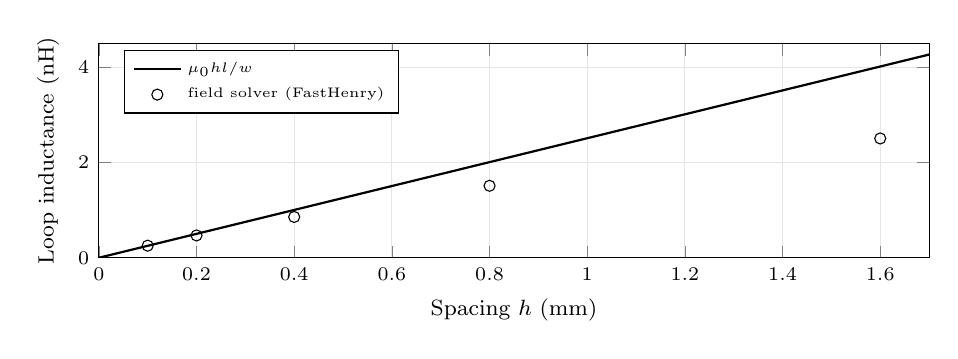
\begin{tikzpicture}
					\begin{axis}[
							width=\linewidth, height=4.3cm,
							xmin=0, xmax=1.7, ymin=0, ymax=4.5,
							xlabel={Spacing $h$ (mm)}, ylabel={Loop inductance (nH)},
							grid=major, grid style={gray!20},
							tick label style={font=\scriptsize}, label style={font=\footnotesize},
							legend style={font=\tiny}, legend pos=north west, legend cell align=left,
						]
						\addplot[black, thick, domain=0:1.7, samples=2] {2.513*x};
						\addlegendentry{$\mu_0hl/w$}
						\addplot[black, only marks, mark=o, mark size=2pt] coordinates {(0.1,0.254) (0.2,0.469) (0.4,0.858) (0.8,1.513) (1.6,2.508)};
						\addlegendentry{field solver (FastHenry)}
					\end{axis}
				\end{tikzpicture}
				\caption{Two copper strips with opposite currents, $w=5$\,mm, $l=10$\,mm, 100\,MHz}
			\end{figure}
		\end{column}
		\begin{column}{0.47\textwidth}
			\small
			Two planes of width $w$ and length $l$, spacing $h\ll w$; the field is confined to the gap:
			\begin{equation*}
				L\approx\mu_0\frac{h\,l}{w}=1.26\,\frac{\mathrm{nH}}{\mathrm{mm}}\cdot\frac{h\,l}{w}
			\end{equation*}
			\begin{itemize}
				\item $h=0.1$\,mm: 0.25\,nH, as the solver.
				\item $h=1.6$\,mm: formula 4.0\,nH, solver 2.5\,nH; at $w/h\approx3$ the field spreads beyond the edges.
			\end{itemize}
			\begin{block}{Key message}
				Return on the adjacent layer: ten times less inductance than across a 1.6\,mm board.
			\end{block}
		\end{column}
	\end{columns}
	\blfootnote{Formula: Lidow et al., 2019, Eq.\ (4.1). Solver results: FastHenry 3.0, computed for this lecture.}
\end{frame}

%%%%%%%%%%%%%%%%%%%%%%%%%%%%%%%%%%%%%%%%%%%%%%%%%%%%%%%%%%%%%
%% Vias and wires %%
%%%%%%%%%%%%%%%%%%%%%%%%%%%%%%%%%%%%%%%%%%%%%%%%%%%%%%%%%%%%%
\begin{frame}
	\frametitle{Vias and wires}
	Partial inductance of a straight round conductor, length $l$, diameter $d$ ($l\gg d$, current at the surface):
	\begin{equation*}
		L_\mathrm{p}\approx\frac{\mu_0 l}{2\pi}\left[\ln\frac{4l}{d}-1\right]=0.2\,\frac{\mathrm{nH}}{\mathrm{mm}}\cdot l\left[\ln\frac{4l}{d}-1\right]
	\end{equation*}
	\begin{columns}[T]
		\begin{column}{0.48\textwidth}
			\centering
			\small
			\begin{tabular}{|l|r|}
				\hline
				\multicolumn{2}{|l|}{\textbf{Partial self-inductance}} \\
				\hline
				via, $l=1.6$\,mm, $d=0.3$\,mm      & 0.7\,nH \\
				bond wire, 2\,mm, 25\,$\mu$m        & 1.9\,nH \\
				wire, 10\,mm, 0.5\,mm              & 6.8\,nH \\
				\hline
			\end{tabular}\\[0.6em]
			\raggedright
			Rule of thumb for thin wires: about 1\,nH per mm.
		\end{column}
		\begin{column}{0.48\textwidth}
			\centering
			\small
			\begin{tabular}{|l|r|}
				\hline
				\multicolumn{2}{|l|}{\textbf{Loop, 1.6\,mm vias, 1\,mm pitch}} \\
				\hline
				1 via pair                         & 1.06\,nH \\
				2 pairs, interleaved               & 0.49\,nH \\
				4 pairs, interleaved               & 0.24\,nH \\
				\hline
			\end{tabular}\\[0.6em]
			\raggedright
			Interleaved forward and return vias act in parallel and cancel each other's field (FastHenry, 100\,MHz).
		\end{column}
	\end{columns}
	\blfootnote{Source: Ott, 2009, Eq.\ (E-14), after Grover, 1946. The often quoted $5.08\,h\,[\ln(4h/d)+1]$\,nH ($h,d$ in inch) gives 1.3\,nH for the via, 1.8 times the solver value.}
\end{frame}

%%%%%%%%%%%%%%%%%%%%%%%%%%%%%%%%%%%%%%%%%%%%%%%%%%%%%%%%%%%%%
%% Spot the loop %%
%%%%%%%%%%%%%%%%%%%%%%%%%%%%%%%%%%%%%%%%%%%%%%%%%%%%%%%%%%%%%
% Two pages: question (page 1) and answer (page 2).
\begin{frame}<handout:1-2>
	\frametitle{Spot the loop}
	Both power loops use 4\,mm wide copper and four vias at each end. Which one has the lower loop inductance? Vote.
	\begin{figure}
		\centering
		\begin{tikzpicture}[x=0.55cm, y=1cm, font=\scriptsize]
			% layout A: 10 mm loop, plane 0.1 mm below
			\fill[gray!15] (-1.6,-0.1) rectangle (11.4,0.0);
			\fill[gray!60] (-1.6,-0.17) rectangle (11.4,-0.1);
			\fill[gray!60] (0,0) rectangle (10,0.07);
			\fill[gray!60] (-1.2,0) rectangle (-0.4,0.07);
			\draw[thick] (9.6,0.07) -- (9.6,-0.1);
			\draw[thick] (-0.8,0.07) -- (-0.8,-0.1);
			\draw[-{Latex[length=1.6mm]}] (0.5,0.25) -- (9,0.25);
			\draw[-{Latex[length=1.6mm]}] (9,-0.4) -- (0.5,-0.4);
			\node[anchor=south] at (-0.8,0.1) {$C_\mathrm{in}$};
			\node[anchor=south] at (10.2,0.1) {switches};
			\node[anchor=north] at (5,-0.45) {return on the first inner layer, 0.1\,mm below};
			\node[anchor=east] at (-2.0,0) {\small\textbf{A}};
			% layout B: 3 mm loop, plane 1.6 mm below
			\begin{scope}[xshift=8.6cm]
				\fill[gray!15] (-1.6,-1.6) rectangle (4.6,0.0);
				\fill[gray!60] (-1.6,-1.67) rectangle (4.6,-1.6);
				\fill[gray!60] (0,0) rectangle (3,0.07);
				\fill[gray!60] (-1.2,0) rectangle (-0.4,0.07);
				\draw[thick] (2.6,0.07) -- (2.6,-1.6);
				\draw[thick] (-0.8,0.07) -- (-0.8,-1.6);
				\draw[-{Latex[length=1.6mm]}] (0.2,0.25) -- (2.4,0.25);
				\draw[-{Latex[length=1.6mm]}] (2.4,-1.9) -- (0.2,-1.9);
				\node[anchor=south] at (-0.8,0.1) {$C_\mathrm{in}$};
				\node[anchor=south] at (3.0,0.1) {switches};
				\node[anchor=north] at (1.5,-1.95) {return on the bottom layer, 1.6\,mm below};
				\node[anchor=east] at (-2.0,0) {\small\textbf{B}};
			\end{scope}
		\end{tikzpicture}
		\caption{Side views; A: loop 10\,mm long, B: loop 3\,mm long (vertical scale 1.8 times the horizontal)}
	\end{figure}
	\onslide<2-|handout:2>{
		\begin{block}{Answer: A}
			FastHenry at 100\,MHz: A 0.47\,nH, B 1.4\,nH. What counts is the area between forward and return current, $10\cdot0.1=1\,\mathrm{mm^2}$ for A and $3\cdot1.6=4.8\,\mathrm{mm^2}$ for B, not the length of the loop.
		\end{block}
	}
\end{frame}

%%%%%%%%%%%%%%%%%%%%%%%%%%%%%%%%%%%%%%%%%%%%%%%%%%%%%%%%%%%%%
%% Switch-node capacitance %%
%%%%%%%%%%%%%%%%%%%%%%%%%%%%%%%%%%%%%%%%%%%%%%%%%%%%%%%%%%%%%
\begin{frame}
	\frametitle{Switch-node capacitance}
	\begin{columns}[T]
		\begin{column}{0.5\textwidth}
			\begin{figure}
				\centering
				\begin{tikzpicture}[font=\scriptsize]
					% board (not to scale)
					\fill[gray!15] (0,0) rectangle (5.0,2.0);
					\fill[gray!60] (0,1.2) rectangle (5.0,1.28);
					\node[anchor=west] at (5.05,1.24) {L2: PGND};
					% switch-node copper on top and bottom, thermal vias
					\fill[gray!60] (1.3,2.0) rectangle (3.7,2.08);
					\fill[gray!60] (1.3,-0.08) rectangle (3.7,0);
					\foreach \x in {1.7,2.2,2.7,3.2} {\fill[gray!60] (\x,0) rectangle ++(0.1,2.0);}
					% device
					\draw[fill=white] (1.8,2.08) rectangle (3.2,2.45);
					\node at (2.5,2.27) {GaN};
					\node[anchor=west] at (3.75,2.25) {switch node};
					% thermal interface and heat sink
					\fill[gray!30] (1.0,-0.68) rectangle (4.0,-0.08);
					\draw[fill=gray!45] (0,-1.25) rectangle (5.0,-0.68);
					\node at (2.5,-0.965) {heat sink (earthed)};
					\node[anchor=west] at (5.05,-0.38) {thermal interface};
					% capacitances
					\begin{scope}[circuitikz/bipoles/length=0.75cm]
						\draw[densely dashed] (1.3,2.04) -- (0.6,2.04);
						\draw (0.6,2.04) to[C, l_=$C_1$] (0.6,1.28);
						\draw[densely dashed] (3.7,-0.04) -- (4.5,-0.04);
						\draw (4.5,-0.04) to[C, l_=$C_2$] (4.5,-0.68);
					\end{scope}
				\end{tikzpicture}
				\caption{High-side switch: its source is the switch node (not to scale)}
			\end{figure}
		\end{column}
		\begin{column}{0.47\textwidth}
			\small
			Parallel-plate estimate $C=\varepsilon_0\varepsilon_\mathrm{r}A/h$:
			\begin{itemize}
				\item $C_1$: 10\,mm $\times$ 10\,mm over PGND at 0.1\,mm, FR-4 ($\varepsilon_\mathrm{r}\approx4.4$): 39\,pF
				\item $C_2$: 30\,mm$^2$ on a 0.2\,mm thermal interface ($\varepsilon_\mathrm{r}\approx5$): 7\,pF
			\end{itemize}
			Consequences at every edge:
			\begin{itemize}
				\item $C_1$ adds to $C_\mathrm{oss}$: extra hard-switching loss $\frac12C_1V^2f_\mathrm{sw}$, 0.045\,W at 48\,V but 3.1\,W at 400\,V (1\,MHz)
				\item $C_2$ to earth: common-mode current $C_2\,\mathrm{d}v/\mathrm{d}t$, 0.7\,A at 100\,V/ns, a main source of common-mode EMI (L14)
			\end{itemize}
			Rule of thumb: 10\,pF at 100\,V/ns give 1\,A.
		\end{column}
	\end{columns}
\end{frame}

%%%%%%%%%%%%%%%%%%%%%%%%%%%%%%%%%%%%%%%%%%%%%%%%%%%%%%%%%%%%%
%% Capacitor mounting %%
%%%%%%%%%%%%%%%%%%%%%%%%%%%%%%%%%%%%%%%%%%%%%%%%%%%%%%%%%%%%%
\begin{frame}
	\frametitle{Capacitor mounting}
	\begin{columns}[T]
		\begin{column}{0.46\textwidth}
			\begin{figure}
				\centering
				\begin{tikzpicture}[font=\scriptsize, scale=1.15]
					\fill[gray!15] (0,0) rectangle (5,0.9);
					\fill[gray!60] (0,0.62) rectangle (5,0.7);
					\node[anchor=west] at (5.05,0.66) {L2};
					% pads and capacitor body
					\fill[gray!60] (1.0,0.9) rectangle (1.8,0.98);
					\fill[gray!60] (3.2,0.9) rectangle (4.0,0.98);
					\draw[fill=white] (1.2,0.98) rectangle (3.8,1.6);
					\foreach \x in {1.5,1.8,...,3.5} {\draw[gray] (\x,1.05) -- (\x,1.53);}
					\node[anchor=south] at (2.5,1.62) {MLCC};
					% via to the plane at the right pad
					\fill[gray!60] (3.55,0.62) rectangle (3.65,0.9);
					% current path
					\draw[-{Latex[length=1.5mm]}] (0.2,1.12) -- (1.0,1.12) -- (1.15,1.3);
					\draw[-{Latex[length=1.5mm]}] (3.6,0.9) -- (3.6,0.45);
					\draw[-{Latex[length=1.5mm]}] (3.4,0.45) -- (0.3,0.45);
					\node[anchor=north] at (2.5,0.0) {current: pad, body, via, plane};
				\end{tikzpicture}
				\caption{Decoupling capacitor in the power loop (side view)}
			\end{figure}
		\end{column}
		\begin{column}{0.51\textwidth}
			\small
			Inductance in series with a decoupling capacitor: the body (ESL in the datasheet, measured on the vendor's fixture), pads, traces and vias, and current spreading in the planes. The body is usually the smallest part.
			\begin{itemize}
				\item vias at or in the pads, return plane on the adjacent layer
				\item several small capacitors in parallel, each with its own vias
				\item reverse geometry (terminals on the long side, e.g.\ 0306 instead of 0603): 50--80\,\% lower ESL according to manufacturers
			\end{itemize}
		\end{column}
	\end{columns}
	\blfootnote{Sources: Ott, 2009, Sec.\ 11.3; manufacturer information on reverse-geometry MLCCs (Yageo, NIC Components).}
\end{frame}

%%%%%%%%%%%%%%%%%%%%%%%%%%%%%%%%%%%%%%%%%%%%%%%%%%%%%%%%%%%%%
%% Tool chain %%
%%%%%%%%%%%%%%%%%%%%%%%%%%%%%%%%%%%%%%%%%%%%%%%%%%%%%%%%%%%%%
\begin{frame}
	\frametitle{From estimate to field solver}
	\begin{table}
		\centering
		\small
		\begin{tabular}{|>{\raggedright\arraybackslash}p{3.0cm}|>{\raggedright\arraybackslash}p{4.6cm}|>{\raggedright\arraybackslash}p{4.8cm}|}
			\hline
			\textbf{Step}                & \textbf{Tool}                                             & \textbf{Use}                                                   \\
			\hline
			Hand estimate                & formulas of this lecture                                  & stack-up and placement                                         \\
			Quasi-static field solver    & FastHenry (inductance), FasterCap (capacitance), both open source; Ansys Q3D & values of the routed layout              \\
			Circuit simulation           & SPICE with device models and extracted parasitics         & ringing, overshoot, losses                                     \\
			Measurement                  & ringing frequency, double-pulse test                      & check of the extracted values (L5)                             \\
			\hline
		\end{tabular}
	\end{table}
	\begin{itemize}
		\item Extract at the ringing frequency (100\,MHz to 1\,GHz): the current flows on the facing copper surfaces.
		\item Device models contain no layout inductance. Add it in SPICE together with a resistance that represents the damping at $f_\mathrm{r}$ (skin effect, capacitor ESR).
	\end{itemize}
	\blfootnote{Sources: Kamon, Tsuk, White, IEEE Trans.\ MTT, vol.\ 42, no.\ 9, 1994 (FastHenry); Lidow et al., 2019, Sec.\ 5.2.}
\end{frame}

%%%%%%%%%%%%%%%%%%%%%%%%%%%%%%%%%%%%%%%%%%%%%%%%%%%%%%%%%%%%%
%% Consequences %%
%%%%%%%%%%%%%%%%%%%%%%%%%%%%%%%%%%%%%%%%%%%%%%%%%%%%%%%%%%%%%
\subsection{Consequences}

\begin{frame}
	\frametitle{Ringing of the power loop}
	\begin{columns}[T]
		\begin{column}{0.5\textwidth}
			\begin{figure}
				\centering
				\begin{tikzpicture}
					\begin{axis}[
							width=\linewidth, height=4.6cm,
							xmin=-1, xmax=10, ymin=-5, ymax=95,
							xlabel={$t$ (ns)}, ylabel={$v_\mathrm{sw}$ (V)},
							grid=major, grid style={gray!20},
							tick label style={font=\scriptsize}, label style={font=\footnotesize},
						]
						\addplot[black, thick] table[x=t, y=v16] {fig/lec03/ring_turn_on.dat};
						\addplot[black, densely dotted, domain=-1:10, samples=2] {48};
						\draw[{Latex[length=1.5mm]}-{Latex[length=1.5mm]}] (axis cs:2.55,89) -- (axis cs:6.6,89) node[midway, below, font=\scriptsize] {$T_\mathrm{r}=1/f_\mathrm{r}$};
					\end{axis}
				\end{tikzpicture}
				\caption{Hard turn-on, switch-node voltage; 48\,V, $L_\mathrm{loop}=1.6$\,nH, $C=260$\,pF, $t_\mathrm{r}=1$\,ns (model)}
			\end{figure}
		\end{column}
		\begin{column}{0.47\textwidth}
			\small
			Every transition excites the series resonance of $L_\mathrm{loop}$ with the capacitance across the switch that is off:
			\begin{equation*}
				f_\mathrm{r}=\frac{1}{2\pi\sqrt{L_\mathrm{loop}C}},\quad Z_0=\sqrt{\frac{L_\mathrm{loop}}{C}}
			\end{equation*}
			with $C=C_\mathrm{oss}(V_\mathrm{DC})+C_\mathrm{par}$ (small-signal value, plus layout and probe).
			\begin{itemize}
				\item 1\,nH and 250\,pF: $f_\mathrm{r}=318$\,MHz, $Z_0=2\,\Omega$
				\item Measured, EPC2022 half-bridge at 48\,V: 438\,MHz with $C\approx710$\,pF, i.e.\ $L_\mathrm{loop}\approx0.2$\,nH
			\end{itemize}
			The ring appears as a peak in the EMI spectrum; measuring it needs a bandwidth above $f_\mathrm{r}$ (L5).
		\end{column}
	\end{columns}
	\blfootnote{Source of the measurement: Lidow et al., 2019, Sec.\ 5.3.}
\end{frame}

%%%%%%%%%%%%%%%%%%%%%%%%%%%%%%%%%%%%%%%%%%%%%%%%%%%%%%%%%%%%%
%% Overshoot %%
%%%%%%%%%%%%%%%%%%%%%%%%%%%%%%%%%%%%%%%%%%%%%%%%%%%%%%%%%%%%%
\begin{frame}
	\frametitle{Overshoot}
	\begin{columns}[T]
		\begin{column}{0.48\textwidth}
			\begin{figure}
				\centering
				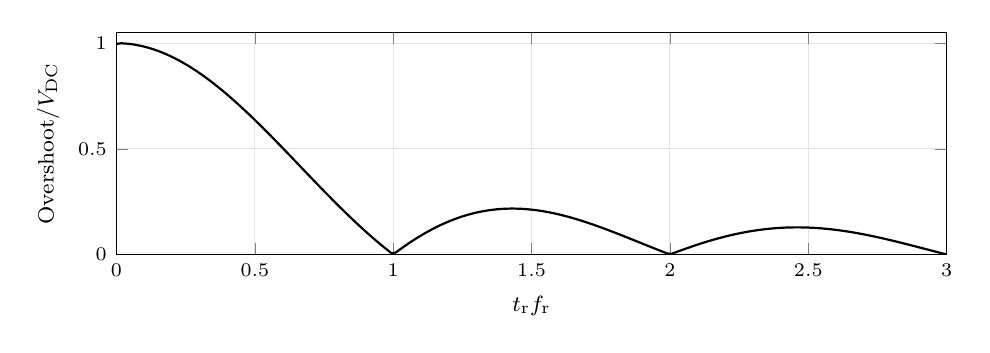
\begin{tikzpicture}
					\begin{axis}[
							width=\linewidth, height=4.4cm,
							xmin=0, xmax=3, ymin=0, ymax=1.05,
							xlabel={$t_\mathrm{r}f_\mathrm{r}$}, ylabel={Overshoot$/V_\mathrm{DC}$},
							grid=major, grid style={gray!20},
							tick label style={font=\scriptsize}, label style={font=\footnotesize},
						]
						\addplot[black, thick, domain=0.001:3, samples=200] {abs(sin(deg(pi*x)))/(pi*x)};
					\end{axis}
				\end{tikzpicture}
				\caption{Voltage step with a linear edge $t_\mathrm{r}$ into an undamped $LC$ circuit}
			\end{figure}
		\end{column}
		\begin{column}{0.49\textwidth}
			\small
			\textbf{Turn-on} of the other switch charges $C$ through $L_\mathrm{loop}$:
			\begin{itemize}
				\item step: up to $2V_\mathrm{DC}$, i.e.\ 100\,\% overshoot
				\item edges slower than $1/f_\mathrm{r}$ excite little ringing
			\end{itemize}
			\textbf{Turn-off} with current $I$: the loop current must stop.
			\begin{itemize}
				\item slow current fall $t_\mathrm{f}\gg1/f_\mathrm{r}$: $\Delta V\approx L_\mathrm{loop}I/t_\mathrm{f}$
				\item any speed (lossless bound): $\Delta V\leq I\,Z_0$
			\end{itemize}
			Measured on a 12\,V GaN buck: 100\,\% overshoot with $L_\mathrm{loop}=1.6$\,nH, 25\,\% with 0.4\,nH. For a fixed rating, overshoot limits the usable input voltage.
		\end{column}
	\end{columns}
	\blfootnote{Sources: Kassakian et al., Principles of Power Electronics, 2nd ed., 2023, Eq.\ (22.1); Reusch and Strydom, IEEE TPEL, 2014.}
\end{frame}

%%%%%%%%%%%%%%%%%%%%%%%%%%%%%%%%%%%%%%%%%%%%%%%%%%%%%%%%%%%%%
%% Your turn: ring and overshoot %%
%%%%%%%%%%%%%%%%%%%%%%%%%%%%%%%%%%%%%%%%%%%%%%%%%%%%%%%%%%%%%
% Two pages: task (page 1) and task with solution (page 2).
\begin{frame}<handout:1-2>
	\frametitle{Ring and overshoot}
	\begin{block}{Task (5 minutes)}
		A GaN half-bridge switches 10\,A at 48\,V. The switch-node voltage rings at 200\,MHz; the datasheet gives $C_\mathrm{oss}=250$\,pF at 48\,V.
		\begin{enumerate}
			\item Estimate the loop inductance.
			\item At turn-off the current falls at 10\,A/ns. Estimate the overshoot with $L\,\mathrm{d}i/\mathrm{d}t$ and with $I\,Z_0$. Which estimate applies?
			\item The switch-node edge at turn-on takes 1\,ns. The devices are rated 100\,V. Is there margin?
		\end{enumerate}
	\end{block}
	\onslide<2-|handout:2>{
		\small
		\begin{enumerate}
			\item $L_\mathrm{loop}=1/\big((2\pi f_\mathrm{r})^2C\big)=1/\big((2\pi\cdot200\,\mathrm{MHz})^2\cdot250\,\mathrm{pF}\big)=2.5$\,nH; ringing period $T_\mathrm{r}=5$\,ns.
			\item $L\,\mathrm{d}i/\mathrm{d}t=25$\,V; $Z_0=3.2\,\Omega$, $I Z_0=32$\,V. The current falls within 1\,ns, much faster than $T_\mathrm{r}$: the bound applies (undamped calculation: 30\,V). $L\,\mathrm{d}i/\mathrm{d}t$ holds only for $t_\mathrm{f}\gg T_\mathrm{r}$.
			\item $t_\mathrm{r}f_\mathrm{r}=0.2$: overshoot up to 94\,\% of 48\,V, i.e.\ a peak near 93\,V (no damping). No margin. A smaller $L_\mathrm{loop}$ raises $f_\mathrm{r}$ and lowers $Z_0$, which helps at both edges.
		\end{enumerate}
	}
\end{frame}

%%%%%%%%%%%%%%%%%%%%%%%%%%%%%%%%%%%%%%%%%%%%%%%%%%%%%%%%%%%%%
%% Energy in the loop inductance %%
%%%%%%%%%%%%%%%%%%%%%%%%%%%%%%%%%%%%%%%%%%%%%%%%%%%%%%%%%%%%%
\begin{frame}
	\frametitle{Loss caused by loop inductance}
	\begin{itemize}
		\item Turn-on: $L_\mathrm{loop}\,\mathrm{d}i/\mathrm{d}t$ lowers the switch voltage while the current rises; part of the turn-on loss is saved.
		\item Turn-off: $\frac12L_\mathrm{loop}I^2$ (100\,nJ for 2\,nH, 10\,A) is dissipated in the switch (slow turn-off) or in the ringing (fast turn-off).
	\end{itemize}
	\begin{table}
		\centering
		\small
		\begin{tabular}{|l|l|l|}
			\hline
			\textbf{Change}                                  & \textbf{Basis} & \textbf{Effect}                                   \\
			\hline
			$L_\mathrm{CS}=1$\,nH                            & calculated     & loss $+50$\,\%                                    \\
			$L_\mathrm{loop}=3$\,nH                          & calculated     & loss $+30$\,\%, partly saved at turn-on           \\
			$L_\mathrm{loop}$ from 0.4 to 2.9\,nH            & measured       & efficiency more than 4\,\% lower                 \\
			$L_\mathrm{loop}$ above 1.4\,nH                  & measured       & overshoot stops rising, switching slows down      \\
			\hline
		\end{tabular}
		\caption{eGaN buck converter 12\,V to 1.2\,V, 20\,A, 1\,MHz (Reusch and Strydom)}
	\end{table}
	\vspace{-0.6em}
	\begin{block}{Key message}
		A large loop inductance causes overshoot, slows the switching and costs efficiency.
	\end{block}
	\blfootnote{Sources: Reusch and Strydom, IEEE TPEL, 2014; on ringing loss: Zhang, Guo, Wang, IEEE TPEL, 2019.}
\end{frame}

%%%%%%%%%%%%%%%%%%%%%%%%%%%%%%%%%%%%%%%%%%%%%%%%%%%%%%%%%%%%%
%% Cgd coupling %%
%%%%%%%%%%%%%%%%%%%%%%%%%%%%%%%%%%%%%%%%%%%%%%%%%%%%%%%%%%%%%
\begin{frame}
	\frametitle{Coupling through $C_\mathrm{GD}$}
	\begin{columns}[T]
		\begin{column}{0.44\textwidth}
			\begin{figure}
				\centering
				\begin{circuitikz}[scale=0.7, transform shape]
					\draw (2.8,1.6) node[nigfete](Q){};
					\draw (Q.D) -- ++(0,0.6) coordinate (d0) -- ++(0,0.6) node[above]{$v_\mathrm{sw}$ rising};
					\draw (Q.S) -- ++(0,-0.6) coordinate (s0) -- ++(0,-0.4) coordinate (gnd) node[ground]{};
					\draw (Q.G) -- ++(-1.0,0) coordinate (g0);
					\draw (g0) to[C, l_=$C_\mathrm{GD}$, *-] (g0 |- d0) -- (d0);
					\draw (g0) to[C, l=$C_\mathrm{GS}$] (g0 |- s0) -- (s0);
					\draw (g0) to[R, l=$R_\mathrm{G,off}$] ++(-2.2,0) coordinate (dv) to[sV, l_=0\,V] (dv |- gnd) -- (gnd);
				\end{circuitikz}
				\caption{Low-side switch, off, while the high-side switch turns on}
			\end{figure}
		\end{column}
		\begin{column}{0.53\textwidth}
			\small
			The switch-node edge drives $i=C_\mathrm{GD}\,\mathrm{d}v/\mathrm{d}t$ into the gate loop:
			\begin{itemize}
				\item edge slow compared with $R_\mathrm{G,off}C_\mathrm{iss}$: $\Delta v_\mathrm{GS}\approx R_\mathrm{G,off}C_\mathrm{GD}\,\mathrm{d}v/\mathrm{d}t$
				\item voltage step (upper bound): $\Delta v_\mathrm{GS}=V_\mathrm{DC}\,C_\mathrm{GD}/(C_\mathrm{GD}+C_\mathrm{GS})$
			\end{itemize}
			Illustrative 650\,V GaN, $C_\mathrm{GD}=2$\,pF, $C_\mathrm{GS}=250$\,pF, $V_\mathrm{th}\approx1.5$\,V, 400\,V at 100\,V/ns:
			\begin{itemize}
				\item $R_\mathrm{G,off}=1\,\Omega$: 0.2\,V, safe
				\item step bound: 3.2\,V, false turn-on
			\end{itemize}
			The off path must keep a low impedance up to hundreds of MHz: short gate loop. Details in L4.
		\end{column}
	\end{columns}
\end{frame}

%%%%%%%%%%%%%%%%%%%%%%%%%%%%%%%%%%%%%%%%%%%%%%%%%%%%%%%%%%%%%
%% Layout rules %%
%%%%%%%%%%%%%%%%%%%%%%%%%%%%%%%%%%%%%%%%%%%%%%%%%%%%%%%%%%%%%
\subsection{Layout rules}

\begin{frame}
	\frametitle{Lateral, vertical and optimal loop}
	\begin{figure}
		\centering
		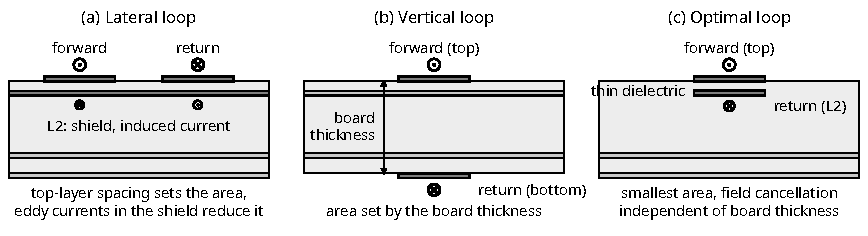
\includegraphics[width=0.92\linewidth]{fig/lec03/pcb_loop_sections.pdf}
		\caption{Cross-sections perpendicular to the loop current (schematic)}
	\end{figure}
	\vspace{-0.4em}
	\begin{table}
		\centering
		\footnotesize
		\begin{tabular}{|>{\raggedright\arraybackslash}p{5.3cm}|>{\raggedright\arraybackslash}p{3.7cm}|>{\raggedright\arraybackslash}p{3.7cm}|}
			\hline
			\textbf{Lateral}: no shield / shield at 0.66 / 0.33 / 0.1\,mm & \textbf{Vertical}: board 1.6 / 0.8\,mm & \textbf{Optimal}: return at 0.3 / 0.1\,mm \\
			3.92 / 2.74 / 2.10 / 1.36\,nH                                  & 2.87 / 1.83\,nH                         & 0.87 / 0.37\,nH                          \\
			\hline
		\end{tabular}
		\caption{Two 3\,mm $\times$ 8\,mm conductors, ideal end connections, FastHenry at 100\,MHz; same trends as in the measurements of Reusch and Strydom}
	\end{table}
\end{frame}

%%%%%%%%%%%%%%%%%%%%%%%%%%%%%%%%%%%%%%%%%%%%%%%%%%%%%%%%%%%%%
%% Optimal power loop %%
%%%%%%%%%%%%%%%%%%%%%%%%%%%%%%%%%%%%%%%%%%%%%%%%%%%%%%%%%%%%%
\begin{frame}
	\frametitle{Optimal power loop}
	\begin{columns}[T]
		\begin{column}{0.5\textwidth}
			\begin{table}
				\centering
				\footnotesize
				\begin{tabular}{|l|c|c|c|}
					\hline
					                                & \textbf{Lat.} & \textbf{Vert.} & \textbf{Opt.} \\
					\hline
					Parts on one side               & yes           & no             & yes           \\
					Field cancellation              & no            & yes            & yes           \\
					$L$ independent of thickness    & yes           & no             & yes           \\
					Shield layer needed             & yes           & no             & no            \\
					\hline
				\end{tabular}
				\caption{Properties of the three loop types}
			\end{table}
			\small
			Four-layer boards, 2\,oz copper (simulation and measurement):
			\begin{itemize}
				\item vertical: $L$ up to 80\,\% higher when the board thickness doubles from 0.8 to 1.6\,mm
				\item lateral: higher loss for the same $L$ (eddy currents in the shield)
			\end{itemize}
		\end{column}
		\begin{column}{0.46\textwidth}
			\small
			Optimal layout: input capacitors next to the drain of the high-side switch, return on the first inner layer directly underneath, rows of interleaved vias between the switches.
			\begin{itemize}
				\item 40\,\% lower loop inductance than the best conventional layout
				\item 35\,\% less overshoot, 10\,\% less loss
				\item full-load efficiency 0.8 and 1\,\% higher than with the vertical and lateral loop
			\end{itemize}
			Integration goes further: a monolithic GaN half-bridge reached about 0.15\,nH, the discrete design 0.25\,nH.
		\end{column}
	\end{columns}
	\blfootnote{Sources: Reusch and Strydom, IEEE TPEL, 2014; Lidow et al., 2019, Sec.\ 4.3, 4.4 and 10.2.}
\end{frame}

%%%%%%%%%%%%%%%%%%%%%%%%%%%%%%%%%%%%%%%%%%%%%%%%%%%%%%%%%%%%%
%% Return current path %%
%%%%%%%%%%%%%%%%%%%%%%%%%%%%%%%%%%%%%%%%%%%%%%%%%%%%%%%%%%%%%
\begin{frame}
	\frametitle{Return current path}
	\begin{columns}[T]
		\begin{column}{0.5\textwidth}
			\begin{figure}
				\centering
				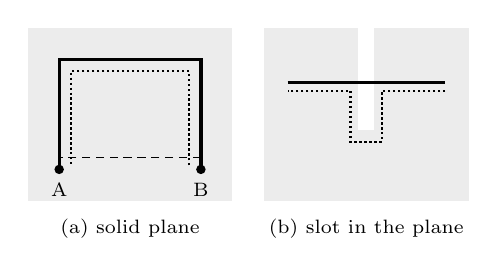
\begin{tikzpicture}[font=\scriptsize]
					% (a) plane with a U-shaped trace
					\fill[gray!15] (0,0) rectangle (2.6,2.2);
					\draw[very thick] (0.4,0.4) -- (0.4,1.8) -- (2.2,1.8) -- (2.2,0.4);
					\fill (0.4,0.4) circle (0.06); \fill (2.2,0.4) circle (0.06);
					\node[anchor=north] at (0.4,0.35) {A}; \node[anchor=north] at (2.2,0.35) {B};
					\draw[densely dashed] (2.2,0.55) -- (0.4,0.55);
					\draw[densely dotted, thick] (2.05,0.45) -- (2.05,1.65) -- (0.55,1.65) -- (0.55,0.45);
					\node at (1.3,-0.35) {(a) solid plane};
					% (b) plane with a slot under the trace
					\begin{scope}[xshift=3.0cm]
						\fill[gray!15] (0,0) rectangle (2.6,2.2);
						\fill[white] (1.2,0.9) rectangle (1.4,2.2);
						\draw[very thick] (0.3,1.5) -- (2.3,1.5);
						\draw[densely dotted, thick] (2.3,1.4) -- (1.5,1.4) -- (1.5,0.75) -- (1.1,0.75) -- (1.1,1.4) -- (0.3,1.4);
						\node at (1.3,-0.35) {(b) slot in the plane};
					\end{scope}
				\end{tikzpicture}
				\caption{Top view: trace (solid), return current at low (dashed) and high frequency (dotted)}
			\end{figure}
		\end{column}
		\begin{column}{0.47\textwidth}
			\small
			\begin{itemize}
				\item Low frequency: path of least resistance. High frequency: path of least inductance, under the trace. The transition lies at a few hundred kHz.
				\item Current density in the plane, conductor at height $h$:
				      \begin{equation*}
					      K(x)=\frac{I}{\pi h}\cdot\frac{1}{1+(x/h)^2}
				      \end{equation*}
				      50\,\% within $\pm h$, 80\,\% within $\pm3h$.
				\item A slot in the plane forces a detour: more inductance and radiation. No splits under high-frequency currents.
			\end{itemize}
		\end{column}
	\end{columns}
	\blfootnote{Source: Ott, 2009, Sec.\ 3.2; $K(x)$ from the image of the conductor in the plane.}
\end{frame}

%%%%%%%%%%%%%%%%%%%%%%%%%%%%%%%%%%%%%%%%%%%%%%%%%%%%%%%%%%%%%
%% Decoupling capacitors %%
%%%%%%%%%%%%%%%%%%%%%%%%%%%%%%%%%%%%%%%%%%%%%%%%%%%%%%%%%%%%%
\begin{frame}
	\frametitle{Decoupling capacitors}
	\begin{itemize}
		\item Place the high-frequency capacitors inside the power loop, at the drain of the high-side and the source of the low-side switch, on the same side as the switches.
		\item Use several equal capacitors in parallel, each with its own vias: $n$ capacitors give about $1/n$ of the inductance, and the current spreads over a wider path.
		\item Class II ceramics (X7R, X5R) lose a large part of their capacitance under DC bias. Use the DC-bias curve of the manufacturer, not the nominal value. C0G does not lose capacitance but has a low capacitance per volume.
		\item The ceramic capacitors supply the pulsed input current. Size them for ripple voltage and RMS current; the bulk capacitor covers low frequencies and the input filter.
	\end{itemize}
	\begin{block}{Example: buck 48\,V to 12\,V, 10\,A, 1\,MHz ($D=0.25$)}
		RMS current in the ceramic capacitors $I_\mathrm{o}\sqrt{D(1-D)}=4.3$\,A. For 1\,V ripple they need
		$C\geq I_\mathrm{o}D(1-D)/(\Delta V f_\mathrm{sw})=1.9\,\mu$F, effective at 48\,V, i.e.\ after the DC-bias derating.
	\end{block}
\end{frame}

%%%%%%%%%%%%%%%%%%%%%%%%%%%%%%%%%%%%%%%%%%%%%%%%%%%%%%%%%%%%%
%% Anti-resonance %%
%%%%%%%%%%%%%%%%%%%%%%%%%%%%%%%%%%%%%%%%%%%%%%%%%%%%%%%%%%%%%
\begin{frame}
	\frametitle{Bulk and ceramic capacitors}
	\begin{columns}[T]
		\begin{column}{0.52\textwidth}
			\begin{figure}
				\centering
				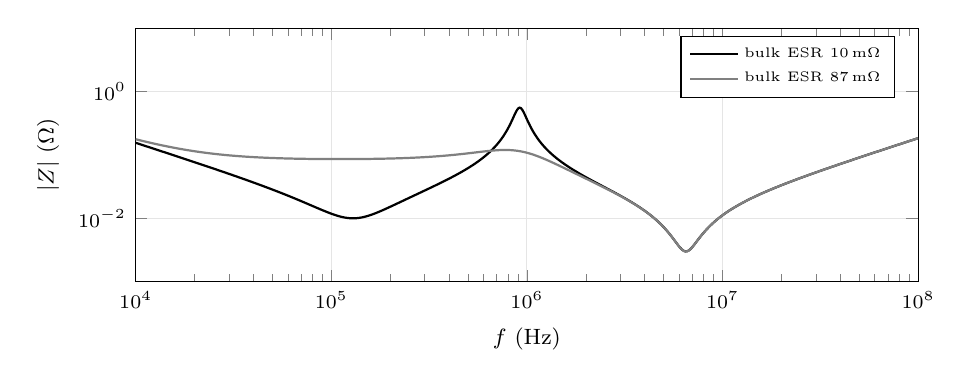
\begin{tikzpicture}[
						declare function={w(\x)=2*pi*10^\x;
								Xa(\x)=w(\x)*0.3e-9-1/(w(\x)*2e-6);
								Xb(\x)=w(\x)*15e-9-1/(w(\x)*100e-6);
								Zp(\x,\ra,\rb)=sqrt(((\ra*\rb-Xa(\x)*Xb(\x))^2+(\ra*Xb(\x)+\rb*Xa(\x))^2)/((\ra+\rb)^2+(Xa(\x)+Xb(\x))^2));}]
					\begin{loglogaxis}[
							width=0.95\linewidth, height=4.8cm,
							xmin=1e4, xmax=1e8, ymin=1e-3, ymax=10,
							xlabel={$f$ (Hz)}, ylabel={$|Z|$ ($\Omega$)},
							grid=major, grid style={gray!20},
							tick label style={font=\scriptsize}, label style={font=\footnotesize},
							legend style={font=\tiny}, legend pos=north east, legend cell align=left,
						]
						\addplot[black, thick, domain=4:8, samples=600] ({10^x}, {Zp(x,0.003,0.010)});
						\addlegendentry{bulk ESR 10\,m$\Omega$}
						\addplot[gray, thick, domain=4:8, samples=600] ({10^x}, {Zp(x,0.003,0.087)});
						\addlegendentry{bulk ESR 87\,m$\Omega$}
					\end{loglogaxis}
				\end{tikzpicture}
				\caption{2\,$\mu$F ceramic (0.3\,nH, 3\,m$\Omega$) in parallel with 100\,$\mu$F bulk (15\,nH including its connection)}
			\end{figure}
		\end{column}
		\begin{column}{0.45\textwidth}
			\small
			Between the two series resonances the ceramic branch is capacitive and the bulk branch inductive: parallel resonance (anti-resonance) at
			\begin{equation*}
				f_\mathrm{ar}\approx\frac{1}{2\pi\sqrt{L_\mathrm{bulk}C_\mathrm{cer}}}=0.92\,\mathrm{MHz}
			\end{equation*}
			Peak 0.56\,$\Omega$, right at a typical $f_\mathrm{sw}$.
			\begin{itemize}
				\item Damping: resistance of about $\sqrt{L_\mathrm{bulk}/C_\mathrm{cer}}=87$\,m$\Omega$ in the bulk branch (e.g.\ an electrolytic capacitor): peak 0.12\,$\Omega$.
				\item Check where $f_\mathrm{ar}$ lies relative to $f_\mathrm{sw}$ and its harmonics.
			\end{itemize}
		\end{column}
	\end{columns}
	\blfootnote{Source: Ott, 2009, Sec.\ 11.4.3 (largest peaks for values an order of magnitude or more apart); values illustrative.}
\end{frame}

%%%%%%%%%%%%%%%%%%%%%%%%%%%%%%%%%%%%%%%%%%%%%%%%%%%%%%%%%%%%%
%% Gate loop layout %%
%%%%%%%%%%%%%%%%%%%%%%%%%%%%%%%%%%%%%%%%%%%%%%%%%%%%%%%%%%%%%
\begin{frame}
	\frametitle{Gate loop layout}
	\begin{columns}[T]
		\begin{column}{0.45\textwidth}
			\begin{figure}
				\centering
				\begin{tikzpicture}[font=\scriptsize]
					% driver and transistor
					\draw (0,0.6) rectangle (1.2,2.0); \node[align=center] at (0.6,1.3) {gate\\driver};
					\draw[fill=gray!15] (2.8,0.2) rectangle (4.4,2.4); \node at (3.6,2.65) {GaN};
					% gate and Kelvin return as a pair
					\draw[very thick] (1.2,1.55) -- (2.8,1.55);
					\draw[very thick, gray] (1.2,1.15) -- (2.8,1.15);
					\node[anchor=south] at (2.0,1.6) {G};
					\node[anchor=north] at (2.0,1.1) {K};
					\draw[-{Latex[length=1.5mm]}] (1.6,1.68) -- (2.4,1.68);
					\draw[-{Latex[length=1.5mm]}] (2.4,1.02) -- (1.6,1.02);
					% driver supply capacitor
					\draw (0.25,0.6) -- (0.25,0.35); \draw (0.95,0.6) -- (0.95,0.35);
					\draw (0.1,0.35) -- (0.4,0.35); \draw (0.1,0.27) -- (0.4,0.27);
					\node[anchor=north] at (0.6,0.2) {$C_\mathrm{VDD}$ at the pins};
					% power current, orthogonal
					\draw[-{Latex[length=2mm]}, thick] (4.0,3.1) -- (4.0,-0.5);
					\node[anchor=west] at (4.1,-0.3) {power current};
				\end{tikzpicture}
				\caption{Top view of driver and transistor (schematic); G gate, K Kelvin source}
			\end{figure}
		\end{column}
		\begin{column}{0.52\textwidth}
			\small
			\begin{itemize}
				\item Driver within a few mm of the gate; gate and return as a pair (side by side or on adjacent layers).
				\item Return to the Kelvin-source pin (chip-scale GaN: the source pads closest to the gate). The gate loop then carries no power current.
				\item Gate loop perpendicular to the power loop, or with opposite currents.
				\item Driver supply capacitor directly at the driver pins.
				\item A small gate-loop inductance allows a small $R_\mathrm{G}$ without gate ringing: $R_\mathrm{G}\geq2\sqrt{L_\mathrm{G}/C_\mathrm{GS}}$ (L4).
			\end{itemize}
		\end{column}
	\end{columns}
	\blfootnote{Source: Lidow et al., 2019, Sec.\ 3.3 and 4.2.}
\end{frame}

%%%%%%%%%%%%%%%%%%%%%%%%%%%%%%%%%%%%%%%%%%%%%%%%%%%%%%%%%%%%%
%% Layer stack-up %%
%%%%%%%%%%%%%%%%%%%%%%%%%%%%%%%%%%%%%%%%%%%%%%%%%%%%%%%%%%%%%
\begin{frame}
	\frametitle{Layer stack-up}
	\begin{columns}[T]
		\begin{column}{0.55\textwidth}
			\begin{figure}
				\centering
				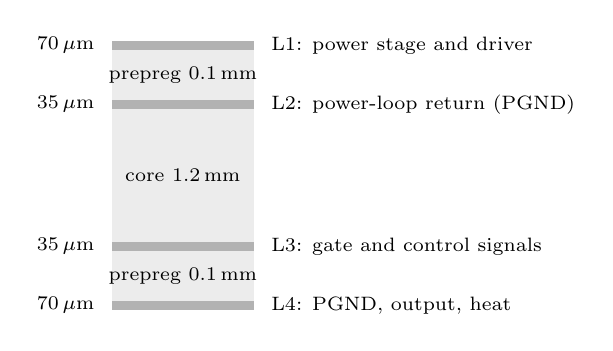
\begin{tikzpicture}[font=\scriptsize]
					% laminate (not to scale)
					\fill[gray!15] (0,0.12) rectangle (1.8,0.75);
					\fill[gray!15] (0,0.87) rectangle (1.8,2.55);
					\fill[gray!15] (0,2.67) rectangle (1.8,3.3);
					\foreach \y/\name/\cu in {3.3/{L1: power stage and driver}/70, 2.55/{L2: power-loop return (PGND)}/35, 0.75/{L3: gate and control signals}/35, 0.0/{L4: PGND, output, heat}/70} {
						\fill[gray!60] (0,\y) rectangle (1.8,\y+0.12);
						\node[anchor=west] at (1.9,\y+0.06) {\name};
						\node[anchor=east] at (-0.1,\y+0.06) {\cu\,$\mu$m};
					}
					\node at (0.9,2.98) {prepreg 0.1\,mm};
					\node at (0.9,1.71) {core 1.2\,mm};
					\node at (0.9,0.43) {prepreg 0.1\,mm};
				\end{tikzpicture}
				\caption{Example 4-layer stack-up, 1.6\,mm, symmetric (not to scale)}
			\end{figure}
		\end{column}
		\begin{column}{0.42\textwidth}
			\small
			\begin{itemize}
				\item Thin dielectric between L1 and L2: return of the power loop, reference of the gate loop.
				\item Signals on L3 have their own reference plane and are shielded from the switch node by L2.
				\item Symmetric build against warping; thick copper outside for current and heat.
				\item Six layers: a second ground plane and more room for control signals.
			\end{itemize}
			Ask the PCB manufacturer for standard prepreg thicknesses and copper weights; they set the loop inductance.
		\end{column}
	\end{columns}
\end{frame}

%%%%%%%%%%%%%%%%%%%%%%%%%%%%%%%%%%%%%%%%%%%%%%%%%%%%%%%%%%%%%
%% Switch-node copper %%
%%%%%%%%%%%%%%%%%%%%%%%%%%%%%%%%%%%%%%%%%%%%%%%%%%%%%%%%%%%%%
\begin{frame}
	\frametitle{Switch-node copper}
	\begin{columns}[T]
		\begin{column}{0.48\textwidth}
			\textbf{Small area}
			\begin{itemize}
				\item less capacitance to planes and heat sink: lower $\frac12CV^2f_\mathrm{sw}$ and common-mode current
				\item less coupling into gate and control signals
				\item 25\,mm$^2$ over L2 at 0.1\,mm are already 10\,pF
			\end{itemize}
		\end{column}
		\begin{column}{0.48\textwidth}
			\textbf{Large area}
			\begin{itemize}
				\item heat spreading for the high-side switch, whose source pad is the switch node
				\item lower resistance to the output inductor
			\end{itemize}
		\end{column}
	\end{columns}
	\vspace{0.4em}
	\begin{itemize}
		\item Output inductor right next to the switches.
		\item No ground or quiet copper under the switch node and the high-side driver, except the return plane under the power loop.
		\item Cool the high-side switch through thermal vias to a small pad on the bottom layer and an insulating thermal interface, or from the top of the package (top-cooled devices).
	\end{itemize}
	\blfootnote{Source: Lidow et al., 2019, Sec.\ 3.8 and 5.3 (about 10\,pF switch-node capacitance on their 48\,V boards).}
\end{frame}

%%%%%%%%%%%%%%%%%%%%%%%%%%%%%%%%%%%%%%%%%%%%%%%%%%%%%%%%%%%%%
%% Copper and spacing %%
%%%%%%%%%%%%%%%%%%%%%%%%%%%%%%%%%%%%%%%%%%%%%%%%%%%%%%%%%%%%%
\begin{frame}
	\frametitle{Copper and spacing}
	\begin{columns}[T]
		\begin{column}{0.48\textwidth}
			\textbf{Copper weight}
			\begin{table}
				\centering
				\footnotesize
				\begin{tabular}{|l|r|r|}
					\hline
					                      & 1\,oz    & 2\,oz    \\
					\hline
					Thickness             & 35\,$\mu$m & 70\,$\mu$m \\
					m$\Omega$ per square, 20\,$^\circ$C & 0.49 & 0.25 \\
					\hline
				\end{tabular}
			\end{table}
			Skin depth of copper: 66\,$\mu$m at 1\,MHz, 21\,$\mu$m at 10\,MHz, 6.6\,$\mu$m at 100\,MHz. Thicker copper helps the DC and low-frequency current, not the ringing current. Current capacity versus temperature rise: IPC-2152.
		\end{column}
		\begin{column}{0.48\textwidth}
			\textbf{Spacing}
			\begin{table}
				\centering
				\footnotesize
				\begin{tabular}{|l|r|r|}
					\hline
					Conductor spacing        & 31--50\,V & 301--500\,V \\
					\hline
					internal layers          & 0.1\,mm   & 0.25\,mm \\
					external, uncoated       & 0.6\,mm   & 2.5\,mm  \\
					external, coated         & 0.13\,mm  & 0.8\,mm  \\
					\hline
				\end{tabular}
				\caption{Minimum spacing, IPC-2221 (rev.\ B), Tab.\ 6-1}
			\end{table}
			These are functional spacings. Mains-connected products need creepage and clearance for basic or reinforced insulation (IEC 62368-1, IEC 60664-1), which are much larger.
		\end{column}
	\end{columns}
\end{frame}

%%%%%%%%%%%%%%%%%%%%%%%%%%%%%%%%%%%%%%%%%%%%%%%%%%%%%%%%%%%%%
%% Damping and snubbers %%
%%%%%%%%%%%%%%%%%%%%%%%%%%%%%%%%%%%%%%%%%%%%%%%%%%%%%%%%%%%%%
\subsection{Damping and snubbers}

\begin{frame}
	\frametitle{RC snubber}
	\begin{columns}[T]
		\begin{column}{0.48\textwidth}
			\begin{figure}
				\centering
				\begin{tikzpicture}
					\begin{semilogxaxis}[
							width=\linewidth, height=4.5cm,
							xmin=0.1, xmax=10, ymin=0, ymax=1.05,
							xlabel={$R/Z_0$}, ylabel={Damping ratio $\zeta$},
							grid=major, grid style={gray!20},
							tick label style={font=\scriptsize}, label style={font=\footnotesize},
							legend style={font=\tiny}, legend pos=north east, legend cell align=left,
						]
						\addplot[black, thick] table[x=r, y=n10] {fig/lec03/snubber_damping.dat};
						\addlegendentry{$C_\mathrm{s}=10\,C_\mathrm{par}$}
						\addplot[black, thick, dashed] table[x=r, y=n3] {fig/lec03/snubber_damping.dat};
						\addlegendentry{$C_\mathrm{s}=3\,C_\mathrm{par}$}
						\addplot[gray, thick] table[x=r, y=n1] {fig/lec03/snubber_damping.dat};
						\addlegendentry{$C_\mathrm{s}=C_\mathrm{par}$}
					\end{semilogxaxis}
				\end{tikzpicture}
				\caption{Damping of the ring by $R$ and $C_\mathrm{s}$ in series across the switch}
			\end{figure}
		\end{column}
		\begin{column}{0.49\textwidth}
			\small
			\begin{enumerate}
				\item Measure the ring $f_\mathrm{r0}$; add a known $C_\mathrm{add}$ across the switch and measure $f_\mathrm{r1}$:
				      \begin{equation*}
					      C_\mathrm{par}=\frac{C_\mathrm{add}}{(f_\mathrm{r0}/f_\mathrm{r1})^2-1},\quad L=\frac{1}{(2\pi f_\mathrm{r0})^2C_\mathrm{par}}
				      \end{equation*}
				      The frequency halves for $C_\mathrm{add}=3C_\mathrm{par}$.
				\item $R\approx Z_0=\sqrt{L/C_\mathrm{par}}$ and $C_\mathrm{s}\approx3$--$4\,C_\mathrm{par}$ give $\zeta\approx0.5$--0.6.
				\item Added loss: $\frac12C_\mathrm{s}V^2$ per fast edge, at most $C_\mathrm{s}V^2f_\mathrm{sw}$.
			\end{enumerate}
			Small packages for $R$ and $C_\mathrm{s}$, inside the power loop; otherwise their own inductance makes them useless at $f_\mathrm{r}$.
		\end{column}
	\end{columns}
	\blfootnote{Sources: Taylor and Manack, TI SLYT465, 2012; damping curves computed for this lecture.}
\end{frame}

%%%%%%%%%%%%%%%%%%%%%%%%%%%%%%%%%%%%%%%%%%%%%%%%%%%%%%%%%%%%%
%% Snubber or layout %%
%%%%%%%%%%%%%%%%%%%%%%%%%%%%%%%%%%%%%%%%%%%%%%%%%%%%%%%%%%%%%
% Two pages: task (page 1) and task with solution (page 2).
\begin{frame}<handout:1-2>
	\frametitle{Snubber or layout?}
	\begin{block}{Task (4 minutes)}
		The half-bridge of the earlier task (48\,V, 1\,MHz, $C_\mathrm{par}=250$\,pF) has been improved to $L_\mathrm{loop}=1$\,nH.
		\begin{enumerate}
			\item Design an RC snubber with $C_\mathrm{s}=3\,C_\mathrm{par}$.
			\item What does it cost? Compare with the energy $\frac12 L_\mathrm{loop}I^2$ at 10\,A.
		\end{enumerate}
	\end{block}
	\onslide<2-|handout:2>{
		\small
		\begin{enumerate}
			\item $Z_0=\sqrt{1\,\mathrm{nH}/250\,\mathrm{pF}}=2\,\Omega$, so $R=2\,\Omega$ and $C_\mathrm{s}=750$\,pF.
			\item Added loss between $\frac12C_\mathrm{s}V^2f_\mathrm{sw}=0.86$\,W and $C_\mathrm{s}V^2f_\mathrm{sw}=1.7$\,W. The ring itself carries only $\frac12LI^2=50$\,nJ, i.e.\ 0.05\,W at 1\,MHz.
		\end{enumerate}
		\begin{block}{Conclusion}
			At MHz switching a full snubber costs more than the ringing. First reduce $L_\mathrm{loop}$, then accept some ringing, and use a small snubber only where overshoot or EMI demand it.
		\end{block}
	}
\end{frame}

%%%%%%%%%%%%%%%%%%%%%%%%%%%%%%%%%%%%%%%%%%%%%%%%%%%%%%%%%%%%%
%% Ringing demo %%
%%%%%%%%%%%%%%%%%%%%%%%%%%%%%%%%%%%%%%%%%%%%%%%%%%%%%%%%%%%%%
\begin{frame}
	\frametitle{Two loop inductances}
	\begin{columns}[T]
		\begin{column}{0.55\textwidth}
			\begin{figure}
				\centering
				\begin{tikzpicture}
					\begin{axis}[
							width=\linewidth, height=5.0cm,
							xmin=-1, xmax=10, ymin=-5, ymax=90,
							xlabel={$t$ (ns)}, ylabel={$v_\mathrm{sw}$ (V)},
							grid=major, grid style={gray!20},
							tick label style={font=\scriptsize}, label style={font=\footnotesize},
							legend style={font=\tiny}, legend pos=north east, legend cell align=left,
						]
						\addplot[gray, thick] table[x=t, y=v04] {fig/lec03/ring_turn_on.dat};
						\addlegendentry{0.4\,nH}
						\addplot[black, thick] table[x=t, y=v16] {fig/lec03/ring_turn_on.dat};
						\addlegendentry{1.6\,nH}
					\end{axis}
				\end{tikzpicture}
				\caption{Model of the hard turn-on: 48\,V, $C=260$\,pF, $t_\mathrm{r}=1$\,ns, $Q=8$}
			\end{figure}
		\end{column}
		\begin{column}{0.42\textwidth}
			\small
			Same edge, two layouts:
			\begin{itemize}
				\item 0.4\,nH: 494\,MHz, peak 73\,V
				\item 1.6\,nH: 247\,MHz, peak 84\,V
			\end{itemize}
			The smaller loop rings at twice the frequency with less overshoot, because the 1\,ns edge is half a ringing period long.\\[0.4em]
			Demo: measure the ring of a GaN half-bridge with a probe of at least 1\,GHz bandwidth and a short ground spring, and compare it with this model (notebook of Tutorial 3).
		\end{column}
	\end{columns}
\end{frame}

%%%%%%%%%%%%%%%%%%%%%%%%%%%%%%%%%%%%%%%%%%%%%%%%%%%%%%%%%%%%%
%% Key messages %%
%%%%%%%%%%%%%%%%%%%%%%%%%%%%%%%%%%%%%%%%%%%%%%%%%%%%%%%%%%%%%
\begin{frame}
	\frametitle{Key messages}
	\begin{enumerate}
		\item The loop inductance is set by the area between forward and return current. Put the return on the adjacent layer, 0.1\,mm below the power loop.
		\item Hand formulas give the right order of magnitude; a field solver gives the value of the routed layout.
		\item $L_\mathrm{loop}$ and $C_\mathrm{oss}+C_\mathrm{par}$ ring at hundreds of MHz. Overshoot is at most $IZ_0$ at turn-off and $V_\mathrm{DC}$ at turn-on.
		\item Common-source inductance and $C_\mathrm{GD}$ couple the power loop into the gate loop: Kelvin source, short gate loop.
		\item Capacitance $C$ at the switch node costs $\frac12CV^2f_\mathrm{sw}$ in hard switching and carries $C\,\mathrm{d}v/\mathrm{d}t$ as common-mode current.
		\item At MHz, a better layout is cheaper than a snubber.
	\end{enumerate}
\end{frame}

%%%%%%%%%%%%%%%%%%%%%%%%%%%%%%%%%%%%%%%%%%%%%%%%%%%%%%%%%%%%%
%% Exit ticket %%
%%%%%%%%%%%%%%%%%%%%%%%%%%%%%%%%%%%%%%%%%%%%%%%%%%%%%%%%%%%%%
% Two pages: questions (page 1) and answers (page 2).
\begin{frame}<handout:1-2>
	\frametitle{Exit ticket}
	\begin{varblock}[\textwidth]{Three questions, one minute each}
		\begin{enumerate}
			\item Which change lowers the loop inductance most: 2\,oz instead of 1\,oz copper, twice the trace width, or the return on L2 instead of L4?
			\item The ringing frequency rises from 200 to 400\,MHz after a layout change, with the same devices. By which factor did $L_\mathrm{loop}$ change?
			\item Why is a large switch-node copper area a problem at 400\,V?
		\end{enumerate}
	\end{varblock}
	\onslide<2-|handout:2>{
		\begin{enumerate}
			\item The return on L2: the spacing drops from about 1.6\,mm to 0.1\,mm. Twice the width roughly halves $L$; the copper thickness hardly matters.
			\item $f_\mathrm{r}\propto1/\sqrt{L}$: four times lower.
			\item Its capacitance adds $\frac12CV^2f_\mathrm{sw}$ of hard-switching loss and $C\,\mathrm{d}v/\mathrm{d}t$ of common-mode current, both large at high voltage.
		\end{enumerate}
	}
\end{frame}

%%%%%%%%%%%%%%%%%%%%%%%%%%%%%%%%%%%%%%%%%%%%%%%%%%%%%%%%%%%%%
%% References %%
%%%%%%%%%%%%%%%%%%%%%%%%%%%%%%%%%%%%%%%%%%%%%%%%%%%%%%%%%%%%%
\begin{frame}
	\frametitle{References}
	\scriptsize
	\begin{itemize}
		\item D. Reusch, J. Strydom, ``Understanding the effect of PCB layout on circuit performance in a high-frequency gallium-nitride-based point of load converter,'' IEEE Trans.\ Power Electron., vol.\ 29, no.\ 4, pp.\ 2008--2015, 2014.
		\item A. Lidow, M. de Rooij, J. Strydom, D. Reusch, J. Glaser, \textit{GaN Transistors for Efficient Power Conversion}, 3rd ed., Wiley, 2019, Ch.\ 3--5 and 10.
		\item H.\,W. Ott, \textit{Electromagnetic Compatibility Engineering}, Wiley, 2009, Ch.\ 3, 11 and App.\ E.
		\item Z. Zhang, B. Guo, F. Wang, L.\,M. Tolbert, B.\,J. Blalock, Z. Liang, P. Ning, ``Methodology for switching characterization evaluation of wide band-gap devices in a phase-leg configuration,'' IEEE APEC 2014, pp.\ 2534--2541.
		\item Z. Zhang, B. Guo, F. Wang, ``Evaluation of switching loss contributed by parasitic ringing for fast switching wide band-gap devices,'' IEEE Trans.\ Power Electron., vol.\ 34, no.\ 9, pp.\ 9082--9094, 2019.
		\item J.\,G. Kassakian, D.\,J. Perreault, G.\,C. Verghese, M.\,F. Schlecht, \textit{Principles of Power Electronics}, 2nd ed., Cambridge University Press, 2023, Ch.\ 22 and 24.
		\item E. Bogatin, \textit{Signal and Power Integrity -- Simplified}, 3rd ed., Pearson, 2018.
		\item M. Kamon, M.\,J. Tsuk, J.\,K. White, ``FASTHENRY: A multipole-accelerated 3-D inductance extraction program,'' IEEE Trans.\ Microw.\ Theory Techn., vol.\ 42, no.\ 9, pp.\ 1750--1758, 1994.
		\item R. Taylor, R. Manack, ``Controlling switch-node ringing in synchronous buck converters,'' TI Analog Applications Journal, SLYT465, 2012.
		\item IPC-2221B, \textit{Generic Standard on Printed Board Design}; IPC-2152, \textit{Standard for Determining Current Carrying Capacity in Printed Board Design}.
	\end{itemize}
\end{frame}
 % Parasitics and PCB layout of the HF commutation cell
%\include{tex/Lecture04} % Gate drivers for fast-switching devices
%\include{tex/Lecture05} % Measurement and characterisation at high frequency
%\include{tex/Lecture06} % HF magnetics I: materials, core loss and the performance factor
%\include{tex/Lecture07} % HF magnetics II: windings, planar and integrated magnetics
%\include{tex/Lecture08} % Soft switching without resonance
%\include{tex/Lecture09} % Resonant converters I: SRC, PRC, LLC and CLLC
%\include{tex/Lecture10} % Resonant converters II: VHF inverters, rectifiers, matching networks
%\include{tex/Lecture11} % Case studies and teardown session
%\include{tex/Lecture12} % Switched-capacitor and hybrid converters
%\include{tex/Lecture13} % Modelling and control of high-frequency converters
%\include{tex/Lecture14} % EMI, thermal design and integration
%\include{tex/Lecture15} % Synthesis, design showcase and exam preparation
%\include{tex/dict} % English-German dictionary
\end{document}
